\documentclass[]{article}
\usepackage{lmodern}
\usepackage{amssymb,amsmath}
\usepackage{ifxetex,ifluatex}
\usepackage{fixltx2e} % provides \textsubscript
\ifnum 0\ifxetex 1\fi\ifluatex 1\fi=0 % if pdftex
  \usepackage[T1]{fontenc}
  \usepackage[utf8]{inputenc}
\else % if luatex or xelatex
  \ifxetex
    \usepackage{mathspec}
  \else
    \usepackage{fontspec}
  \fi
  \defaultfontfeatures{Ligatures=TeX,Scale=MatchLowercase}
\fi
% use upquote if available, for straight quotes in verbatim environments
\IfFileExists{upquote.sty}{\usepackage{upquote}}{}
% use microtype if available
\IfFileExists{microtype.sty}{%
\usepackage{microtype}
\UseMicrotypeSet[protrusion]{basicmath} % disable protrusion for tt fonts
}{}
\usepackage[margin=1in]{geometry}
\usepackage{hyperref}
\hypersetup{unicode=true,
            pdftitle={Local Policy Recommendations for Crime Reduction},
            pdfauthor={Alexa Bagnard, Joseph Gaustad, Kevin Hartman, Francis Leung; (W203 Wednesday 6:30pm Summer 2019)},
            pdfborder={0 0 0},
            breaklinks=true}
\urlstyle{same}  % don't use monospace font for urls
\usepackage{color}
\usepackage{fancyvrb}
\newcommand{\VerbBar}{|}
\newcommand{\VERB}{\Verb[commandchars=\\\{\}]}
\DefineVerbatimEnvironment{Highlighting}{Verbatim}{commandchars=\\\{\}}
% Add ',fontsize=\small' for more characters per line
\newenvironment{Shaded}{}{}
\newcommand{\AlertTok}[1]{\textcolor[rgb]{1.00,0.00,0.00}{#1}}
\newcommand{\AnnotationTok}[1]{\textcolor[rgb]{0.00,0.50,0.00}{#1}}
\newcommand{\AttributeTok}[1]{#1}
\newcommand{\BaseNTok}[1]{#1}
\newcommand{\BuiltInTok}[1]{#1}
\newcommand{\CharTok}[1]{\textcolor[rgb]{0.00,0.50,0.50}{#1}}
\newcommand{\CommentTok}[1]{\textcolor[rgb]{0.00,0.50,0.00}{#1}}
\newcommand{\CommentVarTok}[1]{\textcolor[rgb]{0.00,0.50,0.00}{#1}}
\newcommand{\ConstantTok}[1]{#1}
\newcommand{\ControlFlowTok}[1]{\textcolor[rgb]{0.00,0.00,1.00}{#1}}
\newcommand{\DataTypeTok}[1]{#1}
\newcommand{\DecValTok}[1]{#1}
\newcommand{\DocumentationTok}[1]{\textcolor[rgb]{0.00,0.50,0.00}{#1}}
\newcommand{\ErrorTok}[1]{\textcolor[rgb]{1.00,0.00,0.00}{\textbf{#1}}}
\newcommand{\ExtensionTok}[1]{#1}
\newcommand{\FloatTok}[1]{#1}
\newcommand{\FunctionTok}[1]{#1}
\newcommand{\ImportTok}[1]{#1}
\newcommand{\InformationTok}[1]{\textcolor[rgb]{0.00,0.50,0.00}{#1}}
\newcommand{\KeywordTok}[1]{\textcolor[rgb]{0.00,0.00,1.00}{#1}}
\newcommand{\NormalTok}[1]{#1}
\newcommand{\OperatorTok}[1]{#1}
\newcommand{\OtherTok}[1]{\textcolor[rgb]{1.00,0.25,0.00}{#1}}
\newcommand{\PreprocessorTok}[1]{\textcolor[rgb]{1.00,0.25,0.00}{#1}}
\newcommand{\RegionMarkerTok}[1]{#1}
\newcommand{\SpecialCharTok}[1]{\textcolor[rgb]{0.00,0.50,0.50}{#1}}
\newcommand{\SpecialStringTok}[1]{\textcolor[rgb]{0.00,0.50,0.50}{#1}}
\newcommand{\StringTok}[1]{\textcolor[rgb]{0.00,0.50,0.50}{#1}}
\newcommand{\VariableTok}[1]{#1}
\newcommand{\VerbatimStringTok}[1]{\textcolor[rgb]{0.00,0.50,0.50}{#1}}
\newcommand{\WarningTok}[1]{\textcolor[rgb]{0.00,0.50,0.00}{\textbf{#1}}}
\usepackage{longtable,booktabs}
\usepackage{graphicx,grffile}
\makeatletter
\def\maxwidth{\ifdim\Gin@nat@width>\linewidth\linewidth\else\Gin@nat@width\fi}
\def\maxheight{\ifdim\Gin@nat@height>\textheight\textheight\else\Gin@nat@height\fi}
\makeatother
% Scale images if necessary, so that they will not overflow the page
% margins by default, and it is still possible to overwrite the defaults
% using explicit options in \includegraphics[width, height, ...]{}
\setkeys{Gin}{width=\maxwidth,height=\maxheight,keepaspectratio}
\IfFileExists{parskip.sty}{%
\usepackage{parskip}
}{% else
\setlength{\parindent}{0pt}
\setlength{\parskip}{6pt plus 2pt minus 1pt}
}
\setlength{\emergencystretch}{3em}  % prevent overfull lines
\providecommand{\tightlist}{%
  \setlength{\itemsep}{0pt}\setlength{\parskip}{0pt}}
\setcounter{secnumdepth}{5}
% Redefines (sub)paragraphs to behave more like sections
\ifx\paragraph\undefined\else
\let\oldparagraph\paragraph
\renewcommand{\paragraph}[1]{\oldparagraph{#1}\mbox{}}
\fi
\ifx\subparagraph\undefined\else
\let\oldsubparagraph\subparagraph
\renewcommand{\subparagraph}[1]{\oldsubparagraph{#1}\mbox{}}
\fi

%%% Use protect on footnotes to avoid problems with footnotes in titles
\let\rmarkdownfootnote\footnote%
\def\footnote{\protect\rmarkdownfootnote}

%%% Change title format to be more compact
\usepackage{titling}

% Create subtitle command for use in maketitle
\providecommand{\subtitle}[1]{
  \posttitle{
    \begin{center}\large#1\end{center}
    }
}

\setlength{\droptitle}{-2em}

  \title{Local Policy Recommendations for Crime Reduction}
    \pretitle{\vspace{\droptitle}\centering\huge}
  \posttitle{\par}
  \subtitle{Final Report}
  \author{Alexa Bagnard, Joseph Gaustad, Kevin Hartman, Francis Leung \\ (W203 Wednesday 6:30pm Summer 2019)}
    \preauthor{\centering\large\emph}
  \postauthor{\par}
      \predate{\centering\large\emph}
  \postdate{\par}
    \date{8/7/2019}

\usepackage{booktabs}
\usepackage{longtable}
\usepackage{array}
\usepackage{multirow}
\usepackage{wrapfig}
\usepackage{float}
\usepackage{colortbl}
\usepackage{pdflscape}
\usepackage{tabu}
\usepackage{threeparttable}
\usepackage{threeparttablex}
\usepackage[normalem]{ulem}
\usepackage{makecell}
\usepackage{xcolor}

\begin{document}
\maketitle
\begin{abstract}
This is our study on crime. Crime does not pay. Lorem ipsum dolor sit
amet, consectetur adipiscing elit, sed do eiusmod tempor incididunt ut
labore et dolore magna aliqua. Ut enim ad minim veniam, quis nostrud
exercitation ullamco laboris nisi ut aliquip ex ea commodo consequat.
Duis aute irure dolor in reprehenderit in voluptate velit esse cillum
dolore eu fugiat nulla pariatur. Excepteur sint occaecat cupidatat non
proident, sunt in culpa qui officia deserunt mollit anim id est laborum.
\end{abstract}

{
\setcounter{tocdepth}{2}
\tableofcontents
}
\hypertarget{introduction}{%
\section{Introduction}\label{introduction}}

\hypertarget{background}{%
\subsection{Background}\label{background}}

In this report, we seek to examine and discuss determinants of crime and
offer recommend actionable policy recommendations for local politicians
running for election at the county level in North Carolina. For our
analysis, we draw on sample data collected from a study by Cornwell and
Trumball, researchers from the University of Georgia and West Virginia
University. Our sample data includes data on crime rates, arrests,
sentences, demographics, local weekly wages, tax revenues and more drawn
from local and federal government data sources. Although the age of the
data may be a potential limitation of our study, we believe the insights
we gather and policy recommendations remain appropriate for local
campaigns today.

Our primary question that will drive our data exploration are to ask
which variables affect crime rate the most.

\hypertarget{the-variables}{%
\subsection{The Variables}\label{the-variables}}

The crime\_v2 dataset provided includes 25 variables of interest.

We include them below for reference by category of interest.

\begin{center}
\textbf{Data Dictionary}
\end{center}

\begin{longtable}[]{@{}ll@{}}
\toprule
Category & Variable\tabularnewline
\midrule
\endhead
Crime Rate & crmrte\tabularnewline
Geographic & county, west, central\tabularnewline
Demographic & urban, density, pctmin80, pctymle\tabularnewline
Economic - Wage & wcon, wtuc, wtrd, wfir, wser, wmfg, wfed, wsta,
wloc\tabularnewline
Economic - Revenue & taxpc\tabularnewline
Law Enforcment & polpc, prbarr, prbconv, mix\tabularnewline
Judicial/Sentencing & prbpris, avgsen\tabularnewline
Time Period & year\tabularnewline
\bottomrule
\end{longtable}

\begin{center}
Table 1: Data Dictionary
\end{center}

The variables above operationalize the conditions we wish to explore and
their affects on crime rate

Chiefly, these break down as follows.

\begin{itemize}
\item
  The Economic variables measures the county's economic activity and
  health (e.g.~opportunity to pursue legal forms of income). These
  variables come in the form of available wages and tax revenue returned
  to the county.
\item
  The Law enforcment variables measures the county's ability to utilize
  law enforcment policy to deter crime. Similarly, the Judicial
  variables also signify impact of deterence to crime.
\item
  The Demographic variables measure the cultural variability that
  represent the social differences between each county, such as urban vs
  rural and minority populations.
\item
  The Geographic elements are categorical. They represent they ways in
  which the population is segmented by geography.
\end{itemize}

\hypertarget{exploratory-data-analysis-eda}{%
\section{Exploratory Data Analysis
(EDA)}\label{exploratory-data-analysis-eda}}

\hypertarget{data-prep-and-exploration}{%
\subsection{Data Prep and Exploration}\label{data-prep-and-exploration}}

We begin our analysis by loading the data set and performing basic
checks and inspections.

\begin{Shaded}
\begin{Highlighting}[]
\NormalTok{dfCrime =}\StringTok{ }\KeywordTok{read.csv}\NormalTok{(}\StringTok{"crime_v2.csv"}\NormalTok{)}
\end{Highlighting}
\end{Shaded}

First, we will remove the missing rows from the dataset.

\begin{Shaded}
\begin{Highlighting}[]
\KeywordTok{nrow}\NormalTok{(dfCrime)}
\end{Highlighting}
\end{Shaded}

\begin{verbatim}
[1] 97
\end{verbatim}

\begin{Shaded}
\begin{Highlighting}[]
\NormalTok{dfCrime <-}\KeywordTok{na.omit}\NormalTok{(dfCrime) }\CommentTok{# omit the NA rows}
\KeywordTok{nrow}\NormalTok{(dfCrime)}
\end{Highlighting}
\end{Shaded}

\begin{verbatim}
[1] 91
\end{verbatim}

Next, we will inspect the data to see if there are duplicate records

\begin{Shaded}
\begin{Highlighting}[]
\NormalTok{dfCrime[}\KeywordTok{duplicated}\NormalTok{(dfCrime),]}
\end{Highlighting}
\end{Shaded}

\begin{verbatim}
   county year    crmrte   prbarr     prbconv  prbpris avgsen      polpc
89    193   87 0.0235277 0.266055 0.588859022 0.423423   5.86 0.00117887
     density    taxpc west central urban pctmin80     wcon     wtuc
89 0.8138298 28.51783    1       0     0  5.93109 285.8289 480.1948
       wtrd     wfir     wser   wmfg   wfed   wsta   wloc       mix
89 268.3836 365.0196 295.9352 295.63 468.26 337.88 348.74 0.1105016
      pctymle
89 0.07819394
\end{verbatim}

A duplicate row exists. We'll remove it.

\begin{Shaded}
\begin{Highlighting}[]
\NormalTok{dfCrime <-}\StringTok{ }\NormalTok{dfCrime[}\OperatorTok{!}\KeywordTok{duplicated}\NormalTok{(dfCrime),] }\CommentTok{# remove the duplicated row}
\end{Highlighting}
\end{Shaded}

We also saw that pbconv was coded as a level. It is not a level but a
ratio. We'll change that now.

\begin{Shaded}
\begin{Highlighting}[]
\NormalTok{dfCrime}\OperatorTok{$}\NormalTok{prbconv<-}\KeywordTok{as.numeric}\NormalTok{(}\KeywordTok{levels}\NormalTok{(dfCrime}\OperatorTok{$}\NormalTok{prbconv))[dfCrime}\OperatorTok{$}\NormalTok{prbconv]}
\end{Highlighting}
\end{Shaded}

We also notice by comparision of pctymle and pctmin80 one of the
variables is off by a factor of 100. We will divide pctmin80 by 100 so
the two variables are in the same unit terms.

\begin{Shaded}
\begin{Highlighting}[]
\NormalTok{dfCrime}\OperatorTok{$}\NormalTok{pctmin80<-dfCrime}\OperatorTok{$}\NormalTok{pctmin80}\OperatorTok{/}\DecValTok{100}
\end{Highlighting}
\end{Shaded}

County was expressed as a number. However, it is a categorical variable
and we will convert it to a factor instead.

\begin{Shaded}
\begin{Highlighting}[]
\NormalTok{dfCrime}\OperatorTok{$}\NormalTok{county<-}\KeywordTok{as.factor}\NormalTok{(dfCrime}\OperatorTok{$}\NormalTok{county)}
\end{Highlighting}
\end{Shaded}

Next we inspect the indicator variables to see if they were coded
correctly.

\begin{Shaded}
\begin{Highlighting}[]
\NormalTok{dfCrime }\OperatorTok\StringTok{ }\KeywordTok{group_by}\NormalTok{(west, central) }\OperatorTok\StringTok{ }\KeywordTok{tally}\NormalTok{()}
\end{Highlighting}
\end{Shaded}

\begin{verbatim}
# A tibble: 4 x 3
# Groups:   west [2]
   west central     n
  <int>   <int> <int>
1     0       0    35
2     0       1    33
3     1       0    21
4     1       1     1
\end{verbatim}

\begin{Shaded}
\begin{Highlighting}[]
\NormalTok{dfCrime }\OperatorTok
\KeywordTok{filter}\NormalTok{(west }\OperatorTok{==}\DecValTok{1} \OperatorTok{&}\StringTok{ }\NormalTok{central }\OperatorTok{==}\DecValTok{1}\NormalTok{)}
\end{Highlighting}
\end{Shaded}

\begin{verbatim}
  county year    crmrte   prbarr prbconv  prbpris avgsen      polpc
1     71   87 0.0544061 0.243119 0.22959 0.379175  11.29 0.00207028
   density    taxpc west central urban pctmin80     wcon     wtuc     wtrd
1 4.834734 31.53658    1       1     0  0.13315 291.4508 595.3719 240.3673
      wfir     wser   wmfg   wfed   wsta   wloc       mix    pctymle
1 348.0254 295.2301 358.95 509.43 359.11 339.58 0.1018608 0.07939028
\end{verbatim}

One county was either mis-coded (with west=1 and central=1), or it truly
belongs to both regions. However, this is very unlikely as the intended
technique is to widen the data and introduce indicator variables for
each category. It is not likley the data was captured for both
categories.

We will need further analysis on this datapoint as it relates to the
rest of the data.

For now, we will encode a new region variable and place the datapoint in
its own category.

\begin{Shaded}
\begin{Highlighting}[]
\CommentTok{#Map central and west to a region code, and create a new category for other}
\CommentTok{# Note that county 71 has both western and central codes}
\NormalTok{dfCrime}\OperatorTok{$}\NormalTok{region <-}\StringTok{ }\KeywordTok{case_when}\NormalTok{ (}
\NormalTok{            (dfCrime}\OperatorTok{$}\NormalTok{central }\OperatorTok{==}\DecValTok{0} \OperatorTok{&}\StringTok{ }\NormalTok{dfCrime}\OperatorTok{$}\NormalTok{west }\OperatorTok{==}\DecValTok{0}\NormalTok{) }\OperatorTok{~}\StringTok{ }\DecValTok{0}\NormalTok{, }\CommentTok{#Eastern, Coastal, Other}
\NormalTok{            (dfCrime}\OperatorTok{$}\NormalTok{central }\OperatorTok{==}\DecValTok{0} \OperatorTok{&}\StringTok{ }\NormalTok{dfCrime}\OperatorTok{$}\NormalTok{west }\OperatorTok{==}\DecValTok{1}\NormalTok{) }\OperatorTok{~}\StringTok{ }\DecValTok{1}\NormalTok{, }\CommentTok{#Western}
\NormalTok{            (dfCrime}\OperatorTok{$}\NormalTok{central }\OperatorTok{==}\DecValTok{1} \OperatorTok{&}\StringTok{ }\NormalTok{dfCrime}\OperatorTok{$}\NormalTok{west }\OperatorTok{==}\DecValTok{0}\NormalTok{) }\OperatorTok{~}\StringTok{ }\DecValTok{2}\NormalTok{, }\CommentTok{#Central}
\NormalTok{            (dfCrime}\OperatorTok{$}\NormalTok{central }\OperatorTok{==}\DecValTok{1} \OperatorTok{&}\StringTok{ }\NormalTok{dfCrime}\OperatorTok{$}\NormalTok{west }\OperatorTok{==}\DecValTok{1}\NormalTok{) }\OperatorTok{~}\StringTok{ }\DecValTok{3} \CommentTok{#Central-Western county?}
\NormalTok{        )}
\NormalTok{dfCrime}\OperatorTok{$}\NormalTok{regcode =}
\StringTok{            }\KeywordTok{factor}\NormalTok{( dfCrime}\OperatorTok{$}\NormalTok{region , }\DataTypeTok{levels =} \DecValTok{0}\OperatorTok{:}\DecValTok{3}\NormalTok{ , }\DataTypeTok{labels =}
                    \KeywordTok{c}\NormalTok{( }\StringTok{'Coastal'}\NormalTok{,}
                       \StringTok{'West'}\NormalTok{,}
                       \StringTok{'Central'}\NormalTok{,}
                       \StringTok{'CW'}\NormalTok{)}
\NormalTok{                   )}
\end{Highlighting}
\end{Shaded}

We will also introduce an indicator variable for counties located in the
``other'' region that are not west or central

\begin{Shaded}
\begin{Highlighting}[]
\NormalTok{dfCrime}\OperatorTok{$}\NormalTok{other <-}\StringTok{ }\KeywordTok{ifelse}\NormalTok{((dfCrime}\OperatorTok{$}\NormalTok{central }\OperatorTok{==}\DecValTok{0} \OperatorTok{&}\StringTok{ }\NormalTok{dfCrime}\OperatorTok{$}\NormalTok{west }\OperatorTok{==}\DecValTok{0}\NormalTok{), }\DecValTok{1}\NormalTok{, }\DecValTok{0}\NormalTok{)}
\end{Highlighting}
\end{Shaded}

And we'll add an indicator variable to serve as complement to the urban
indicator variable and call this `nonurban'

\begin{Shaded}
\begin{Highlighting}[]
\NormalTok{dfCrime}\OperatorTok{$}\NormalTok{nonurban <-}\StringTok{ }\KeywordTok{ifelse}\NormalTok{((dfCrime}\OperatorTok{$}\NormalTok{urban}\OperatorTok{==}\DecValTok{0}\NormalTok{), }\DecValTok{1}\NormalTok{, }\DecValTok{0}\NormalTok{)}
\end{Highlighting}
\end{Shaded}

By way of the 1980 Census fact sheet, we discover the urban field is an
encoding for SMSA (Standard Metropolitan Statistical Areas).
\url{https://www2.census.gov/prod2/decennial/documents/1980/1980censusofpopu8011uns_bw.pdf}
The value is one if the county is inside a metropolitan area. Otherwise,
if the county is outisde a metropolitan area, the value is zero.

We create a metro factor variable to better describe this feature.

\begin{Shaded}
\begin{Highlighting}[]
\CommentTok{# create factor for SMSA (standard metropolitan statistical areas) with two levels }
\CommentTok{# (inside or outside)}
\CommentTok{#    https://www2.census.gov/prod2/decennial/documents/1980/1980censusofpopu8011uns_bw.pdf}
\NormalTok{dfCrime}\OperatorTok{$}\NormalTok{metro =}
\StringTok{            }\KeywordTok{factor}\NormalTok{( dfCrime}\OperatorTok{$}\NormalTok{urban , }\DataTypeTok{levels =} \DecValTok{0}\OperatorTok{:}\DecValTok{1}\NormalTok{ , }\DataTypeTok{labels =}
                    \KeywordTok{c}\NormalTok{( }\StringTok{'Outside Metro'}\NormalTok{,}
                       \StringTok{'Inside Metro'}
\NormalTok{                      )}
\NormalTok{                   )}
\end{Highlighting}
\end{Shaded}

Next we will visualize each variable and its relationship to the
variable crmrte through scatter plots

\begin{Shaded}
\begin{Highlighting}[]
\CommentTok{#Plot of the economic and tax related variables vs crmrte}
\NormalTok{q1<-}\KeywordTok{ggplot}\NormalTok{(}\DataTypeTok{data =}\NormalTok{ dfCrime, }\KeywordTok{aes}\NormalTok{(}\DataTypeTok{x =}\NormalTok{ wcon, }\DataTypeTok{y =}\NormalTok{ crmrte, }\DataTypeTok{color =}\NormalTok{ regcode)) }\OperatorTok{+}\StringTok{ }
\StringTok{      }\KeywordTok{geom_point}\NormalTok{()}\OperatorTok{+}
\StringTok{  }\KeywordTok{geom_smooth}\NormalTok{(}\DataTypeTok{method =} \StringTok{"lm"}\NormalTok{)}
\NormalTok{q2<-}\KeywordTok{ggplot}\NormalTok{(}\DataTypeTok{data =}\NormalTok{ dfCrime, }\KeywordTok{aes}\NormalTok{(}\DataTypeTok{x =}\NormalTok{ wtuc, }\DataTypeTok{y =}\NormalTok{ crmrte, }\DataTypeTok{color =}\NormalTok{ regcode)) }\OperatorTok{+}\StringTok{ }
\StringTok{      }\KeywordTok{geom_point}\NormalTok{()}\OperatorTok{+}
\StringTok{  }\KeywordTok{geom_smooth}\NormalTok{(}\DataTypeTok{method =} \StringTok{"lm"}\NormalTok{)}
\NormalTok{q3<-}\KeywordTok{ggplot}\NormalTok{(}\DataTypeTok{data =}\NormalTok{ dfCrime, }\KeywordTok{aes}\NormalTok{(}\DataTypeTok{x =}\NormalTok{ wtrd, }\DataTypeTok{y =}\NormalTok{ crmrte, }\DataTypeTok{color =}\NormalTok{ regcode)) }\OperatorTok{+}\StringTok{ }
\StringTok{      }\KeywordTok{geom_point}\NormalTok{()}\OperatorTok{+}
\StringTok{  }\KeywordTok{geom_smooth}\NormalTok{(}\DataTypeTok{method =} \StringTok{"lm"}\NormalTok{)}
\NormalTok{q4<-}\KeywordTok{ggplot}\NormalTok{(}\DataTypeTok{data =}\NormalTok{ dfCrime, }\KeywordTok{aes}\NormalTok{(}\DataTypeTok{x =}\NormalTok{ wfir, }\DataTypeTok{y =}\NormalTok{ crmrte, }\DataTypeTok{color =}\NormalTok{ regcode)) }\OperatorTok{+}\StringTok{ }
\StringTok{      }\KeywordTok{geom_point}\NormalTok{()}\OperatorTok{+}
\StringTok{  }\KeywordTok{geom_smooth}\NormalTok{(}\DataTypeTok{method =} \StringTok{"lm"}\NormalTok{)}
\NormalTok{q5<-}\KeywordTok{ggplot}\NormalTok{(}\DataTypeTok{data =}\NormalTok{ dfCrime, }\KeywordTok{aes}\NormalTok{(}\DataTypeTok{x =}\NormalTok{ wser, }\DataTypeTok{y =}\NormalTok{ crmrte, }\DataTypeTok{color =}\NormalTok{ regcode)) }\OperatorTok{+}\StringTok{ }
\StringTok{      }\KeywordTok{geom_point}\NormalTok{()}\OperatorTok{+}
\StringTok{  }\KeywordTok{geom_smooth}\NormalTok{(}\DataTypeTok{method =} \StringTok{"lm"}\NormalTok{)}
\NormalTok{q6<-}\KeywordTok{ggplot}\NormalTok{(}\DataTypeTok{data =}\NormalTok{ dfCrime, }\KeywordTok{aes}\NormalTok{(}\DataTypeTok{x =}\NormalTok{ wmfg, }\DataTypeTok{y =}\NormalTok{ crmrte, }\DataTypeTok{color =}\NormalTok{ regcode)) }\OperatorTok{+}\StringTok{ }
\StringTok{      }\KeywordTok{geom_point}\NormalTok{()}\OperatorTok{+}
\StringTok{  }\KeywordTok{geom_smooth}\NormalTok{(}\DataTypeTok{method =} \StringTok{"lm"}\NormalTok{)}
\NormalTok{q7<-}\KeywordTok{ggplot}\NormalTok{(}\DataTypeTok{data =}\NormalTok{ dfCrime, }\KeywordTok{aes}\NormalTok{(}\DataTypeTok{x =}\NormalTok{ wfed, }\DataTypeTok{y =}\NormalTok{ crmrte, }\DataTypeTok{color =}\NormalTok{ regcode)) }\OperatorTok{+}\StringTok{ }
\StringTok{      }\KeywordTok{geom_point}\NormalTok{()}\OperatorTok{+}
\StringTok{  }\KeywordTok{geom_smooth}\NormalTok{(}\DataTypeTok{method =} \StringTok{"lm"}\NormalTok{)}
\NormalTok{q8<-}\KeywordTok{ggplot}\NormalTok{(}\DataTypeTok{data =}\NormalTok{ dfCrime, }\KeywordTok{aes}\NormalTok{(}\DataTypeTok{x =}\NormalTok{ wsta, }\DataTypeTok{y =}\NormalTok{ crmrte, }\DataTypeTok{color =}\NormalTok{ regcode)) }\OperatorTok{+}\StringTok{ }
\StringTok{      }\KeywordTok{geom_point}\NormalTok{()}\OperatorTok{+}
\StringTok{  }\KeywordTok{geom_smooth}\NormalTok{(}\DataTypeTok{method =} \StringTok{"lm"}\NormalTok{)}
\NormalTok{q9<-}\KeywordTok{ggplot}\NormalTok{(}\DataTypeTok{data =}\NormalTok{ dfCrime, }\KeywordTok{aes}\NormalTok{(}\DataTypeTok{x =}\NormalTok{ wloc, }\DataTypeTok{y =}\NormalTok{ crmrte, }\DataTypeTok{color =}\NormalTok{ regcode)) }\OperatorTok{+}\StringTok{ }
\StringTok{      }\KeywordTok{geom_point}\NormalTok{()}\OperatorTok{+}
\StringTok{  }\KeywordTok{geom_smooth}\NormalTok{(}\DataTypeTok{method =} \StringTok{"lm"}\NormalTok{)}
\NormalTok{q10<-}\KeywordTok{ggplot}\NormalTok{(}\DataTypeTok{data =}\NormalTok{ dfCrime, }\KeywordTok{aes}\NormalTok{(}\DataTypeTok{x =}\NormalTok{ taxpc, }\DataTypeTok{y =}\NormalTok{ crmrte, }\DataTypeTok{color =}\NormalTok{ regcode)) }\OperatorTok{+}\StringTok{ }
\StringTok{      }\KeywordTok{geom_point}\NormalTok{()}\OperatorTok{+}
\StringTok{  }\KeywordTok{geom_smooth}\NormalTok{(}\DataTypeTok{method =} \StringTok{"lm"}\NormalTok{)}
\KeywordTok{grid.arrange}\NormalTok{(q1, q2, q3, q4, q5, q6, q7, q8, q9, q10, }\DataTypeTok{ncol=}\DecValTok{2}\NormalTok{)}
\end{Highlighting}
\end{Shaded}

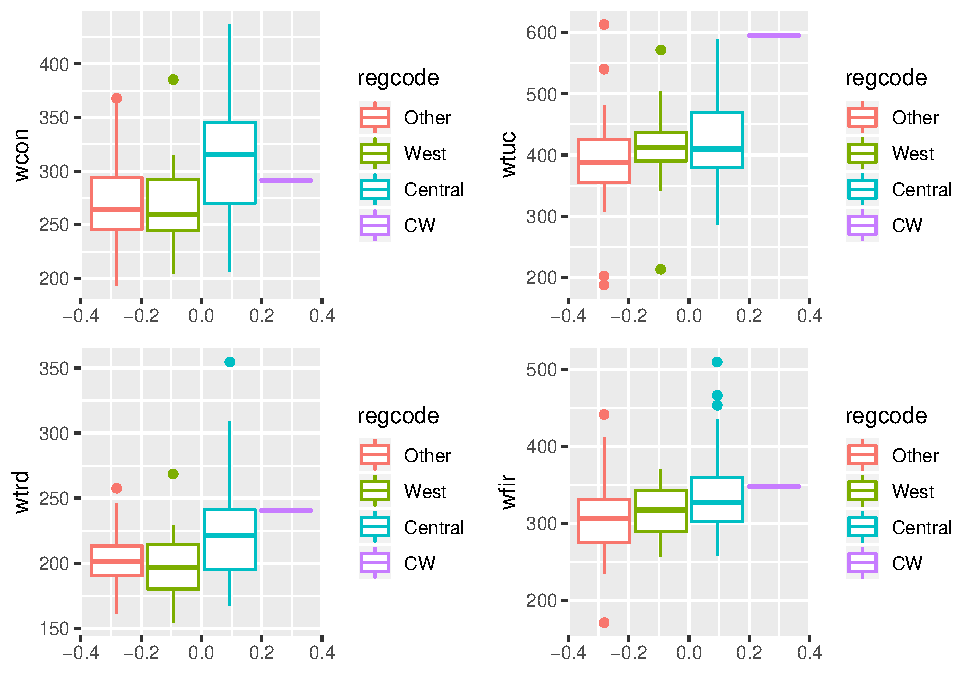
\includegraphics{Bagnard_Gaustad_Hartman_Leung_Lab_3_files/figure-latex/unnamed-chunk-15-1.pdf}

We observe a few data points of interest in the comparison above,
notably, wser appears to have an extreme data point.

Other variables show outliers as well, but not as extreme. We will
determine if any of these points have leverage or influence during model
specification.

For now, lets dig deeper into one of the extreme outliers after our
visual inspection.

\begin{Shaded}
\begin{Highlighting}[]
\NormalTok{dfCrime }\OperatorTok
\KeywordTok{filter}\NormalTok{(wser }\OperatorTok{>}\StringTok{ }\DecValTok{2000}\NormalTok{) }\OperatorTok
\KeywordTok{select}\NormalTok{(county, wser)}
\end{Highlighting}
\end{Shaded}

\begin{verbatim}
  county     wser
1    185 2177.068
\end{verbatim}

This average service wage is much too high based on what we know about
the 1980s and every other wage recorded in comparison. A review of the
detailed population statistics describing mean wage per industry (table
231) confirms this.
\url{https://www2.census.gov/prod2/decennial/documents/1980/1980censusofpopu801352uns_bw.pdf}

Outliers affect our ability to estimate statistics, resulting in
overestimated or underestimated values. Outliers can be due to a number
of different factors such as response errors and data entry errors.
Outliers will introduce bias into our estimates and are addressed during
the analysis phase. The mechanism for treatment include three approaches
1) trimming 2) winsorization or 3) imputation. Trimming will remove the
rest of the values in the observation and is not an preferred treatment.
Winsorazion relies on replacing outliers with the second largest or
second smallest value excluding the outlier. Imputation methods can use
the mean of a variable, or utilize regression models to predict the
missing value. A number of packages are available in R that use the
sample data to predict this value through regression. A full discussion
on treatment methods can be found here:
\url{http://www.asasrms.org/Proceedings/y2004/files/Jsm2004-000559.pdf}

We will use the Hmisc package which contains an impute function for
treatment of this outlier

\begin{Shaded}
\begin{Highlighting}[]
\NormalTok{dfCrime}\OperatorTok{$}\NormalTok{wser[}\KeywordTok{which}\NormalTok{(dfCrime}\OperatorTok{$}\NormalTok{county}\OperatorTok{==}\DecValTok{185}\NormalTok{)]<-}\OtherTok{NA} \CommentTok{# set the value to NA so it will be imputed}
\end{Highlighting}
\end{Shaded}

\begin{Shaded}
\begin{Highlighting}[]
\NormalTok{impute_arg <-}\StringTok{ }\KeywordTok{aregImpute}\NormalTok{(}\OperatorTok{~}\StringTok{ }\NormalTok{crmrte }\OperatorTok{+}\StringTok{  }\NormalTok{urban }\OperatorTok{+}\StringTok{ }\NormalTok{central }\OperatorTok{+}\StringTok{ }\NormalTok{west }\OperatorTok{+}\StringTok{ }\NormalTok{other }\OperatorTok{+}
\StringTok{                         }\NormalTok{prbarr }\OperatorTok{+}\StringTok{ }\NormalTok{prbconv }\OperatorTok{+}\StringTok{ }\NormalTok{prbpris }\OperatorTok{+}\StringTok{ }\NormalTok{avgsen }\OperatorTok{+}\StringTok{ }\NormalTok{polpc }\OperatorTok{+}\StringTok{ }
\StringTok{                         }\NormalTok{density }\OperatorTok{+}\StringTok{ }\NormalTok{taxpc }\OperatorTok{+}\StringTok{ }\NormalTok{pctmin80 }\OperatorTok{+}\StringTok{ }\NormalTok{wcon }\OperatorTok{+}\StringTok{ }\NormalTok{wtuc }\OperatorTok{+}
\StringTok{                         }\NormalTok{wtrd }\OperatorTok{+}\StringTok{ }\NormalTok{wfir }\OperatorTok{+}\StringTok{ }\NormalTok{wser }\OperatorTok{+}\StringTok{ }\NormalTok{wmfg }\OperatorTok{+}\StringTok{ }\NormalTok{wfed }\OperatorTok{+}\StringTok{ }\NormalTok{wsta }\OperatorTok{+}\StringTok{ }\NormalTok{wloc }\OperatorTok{+}
\StringTok{                         }\NormalTok{mix }\OperatorTok{+}\StringTok{ }\NormalTok{pctymle, }\DataTypeTok{data =}\NormalTok{ dfCrime, }\DataTypeTok{match=}\StringTok{"weighted"}\NormalTok{,}
                         \DataTypeTok{nk=}\DecValTok{3}\NormalTok{, }\DataTypeTok{B=}\DecValTok{10}\NormalTok{, }\DataTypeTok{n.impute =} \DecValTok{100}\NormalTok{)}
\end{Highlighting}
\end{Shaded}

\begin{Shaded}
\begin{Highlighting}[]
\KeywordTok{paste}\NormalTok{(}\StringTok{"R-squares for Predicting Non-Missing Values for Each Variable"}\NormalTok{)}
\end{Highlighting}
\end{Shaded}

\begin{verbatim}
[1] "R-squares for Predicting Non-Missing Values for Each Variable"
\end{verbatim}

\begin{Shaded}
\begin{Highlighting}[]
\NormalTok{impute_arg}\OperatorTok{$}\NormalTok{rsq}
\end{Highlighting}
\end{Shaded}

\begin{verbatim}
     wser 
0.8804895 
\end{verbatim}

\begin{Shaded}
\begin{Highlighting}[]
\KeywordTok{paste}\NormalTok{(}\StringTok{"Distribution of Values for Each Imputation"}\NormalTok{)}
\end{Highlighting}
\end{Shaded}

\begin{verbatim}
[1] "Distribution of Values for Each Imputation"
\end{verbatim}

\begin{Shaded}
\begin{Highlighting}[]
\KeywordTok{table}\NormalTok{(impute_arg}\OperatorTok{$}\NormalTok{imputed}\OperatorTok{$}\NormalTok{wser)}
\end{Highlighting}
\end{Shaded}

\begin{verbatim}

133.0430603 172.6280975 182.0196228 192.3076935 196.1453247 203.8864288 
         10           1           2           1           1           1 
204.3792114  206.281601 210.4414825 219.6342773 221.3903351 230.6580658 
          1           2           1           1           1           1 
239.2233429 243.4705658 251.4270172 253.6207123 274.1774597 292.7027283 
          1           1           2           1          69           1 
305.1542664 347.6608887 
          1           1 
\end{verbatim}

We will reassign the value in our dataset to the mean from these trials.

\begin{Shaded}
\begin{Highlighting}[]
\NormalTok{dfCrime}\OperatorTok{$}\NormalTok{wser[}\KeywordTok{which}\NormalTok{(dfCrime}\OperatorTok{$}\NormalTok{county}\OperatorTok{==}\DecValTok{185}\NormalTok{)]<-}\KeywordTok{mean}\NormalTok{(impute_arg}\OperatorTok{$}\NormalTok{imputed}\OperatorTok{$}\NormalTok{wser)}
\KeywordTok{print}\NormalTok{(}\StringTok{"Newly Reassigned wser Value for County 185:"}\NormalTok{)}
\end{Highlighting}
\end{Shaded}

\begin{verbatim}
[1] "Newly Reassigned wser Value for County 185:"
\end{verbatim}

\begin{Shaded}
\begin{Highlighting}[]
\NormalTok{dfCrime}\OperatorTok{$}\NormalTok{wser[}\KeywordTok{which}\NormalTok{(dfCrime}\OperatorTok{$}\NormalTok{county}\OperatorTok{==}\DecValTok{185}\NormalTok{)]}
\end{Highlighting}
\end{Shaded}

\begin{verbatim}
[1] 250.6144
\end{verbatim}

Next, we will examine the criminal justice variables.

\begin{Shaded}
\begin{Highlighting}[]
\CommentTok{#Plot of the criminal justice and law enforcment related variables vs crmrte}
\NormalTok{q1<-}\KeywordTok{ggplot}\NormalTok{(}\DataTypeTok{data =}\NormalTok{ dfCrime, }\KeywordTok{aes}\NormalTok{(}\DataTypeTok{x =}\NormalTok{ prbarr, }\DataTypeTok{y =}\NormalTok{ crmrte, }\DataTypeTok{color =}\NormalTok{ region)) }\OperatorTok{+}\StringTok{ }
\StringTok{      }\KeywordTok{geom_point}\NormalTok{()}\OperatorTok{+}
\StringTok{  }\KeywordTok{geom_smooth}\NormalTok{(}\DataTypeTok{method =} \StringTok{"lm"}\NormalTok{)}
\NormalTok{q2<-}\KeywordTok{ggplot}\NormalTok{(}\DataTypeTok{data =}\NormalTok{ dfCrime, }\KeywordTok{aes}\NormalTok{(}\DataTypeTok{x =}\NormalTok{ prbconv, }\DataTypeTok{y =}\NormalTok{ crmrte, }\DataTypeTok{color =}\NormalTok{ region)) }\OperatorTok{+}\StringTok{ }
\StringTok{      }\KeywordTok{geom_point}\NormalTok{()}\OperatorTok{+}
\StringTok{  }\KeywordTok{geom_smooth}\NormalTok{(}\DataTypeTok{method =} \StringTok{"lm"}\NormalTok{)}
\NormalTok{q3<-}\KeywordTok{ggplot}\NormalTok{(}\DataTypeTok{data =}\NormalTok{ dfCrime, }\KeywordTok{aes}\NormalTok{(}\DataTypeTok{x =}\NormalTok{ prbpris, }\DataTypeTok{y =}\NormalTok{ crmrte, }\DataTypeTok{color =}\NormalTok{ region)) }\OperatorTok{+}\StringTok{ }
\StringTok{      }\KeywordTok{geom_point}\NormalTok{()}\OperatorTok{+}
\StringTok{  }\KeywordTok{geom_smooth}\NormalTok{(}\DataTypeTok{method =} \StringTok{"lm"}\NormalTok{)}
\NormalTok{q4<-}\KeywordTok{ggplot}\NormalTok{(}\DataTypeTok{data =}\NormalTok{ dfCrime, }\KeywordTok{aes}\NormalTok{(}\DataTypeTok{x =}\NormalTok{ avgsen, }\DataTypeTok{y =}\NormalTok{ crmrte, }\DataTypeTok{color =}\NormalTok{ region)) }\OperatorTok{+}\StringTok{ }
\StringTok{      }\KeywordTok{geom_point}\NormalTok{()}\OperatorTok{+}
\StringTok{  }\KeywordTok{geom_smooth}\NormalTok{(}\DataTypeTok{method =} \StringTok{"lm"}\NormalTok{)}
\NormalTok{q5<-}\KeywordTok{ggplot}\NormalTok{(}\DataTypeTok{data =}\NormalTok{ dfCrime, }\KeywordTok{aes}\NormalTok{(}\DataTypeTok{x =}\NormalTok{ polpc, }\DataTypeTok{y =}\NormalTok{ crmrte, }\DataTypeTok{color =}\NormalTok{ region)) }\OperatorTok{+}\StringTok{ }
\StringTok{      }\KeywordTok{geom_point}\NormalTok{()}\OperatorTok{+}
\StringTok{  }\KeywordTok{geom_smooth}\NormalTok{(}\DataTypeTok{method =} \StringTok{"lm"}\NormalTok{)}
\NormalTok{q6<-}\KeywordTok{ggplot}\NormalTok{(}\DataTypeTok{data =}\NormalTok{ dfCrime, }\KeywordTok{aes}\NormalTok{(}\DataTypeTok{x =}\NormalTok{ mix, }\DataTypeTok{y =}\NormalTok{ crmrte, }\DataTypeTok{color =}\NormalTok{ region)) }\OperatorTok{+}\StringTok{ }
\StringTok{      }\KeywordTok{geom_point}\NormalTok{()}\OperatorTok{+}
\StringTok{  }\KeywordTok{geom_smooth}\NormalTok{(}\DataTypeTok{method =} \StringTok{"lm"}\NormalTok{)}

\KeywordTok{grid.arrange}\NormalTok{(q1, q2, q3, q4, q5, q6, }\DataTypeTok{ncol=}\DecValTok{2}\NormalTok{)}
\end{Highlighting}
\end{Shaded}

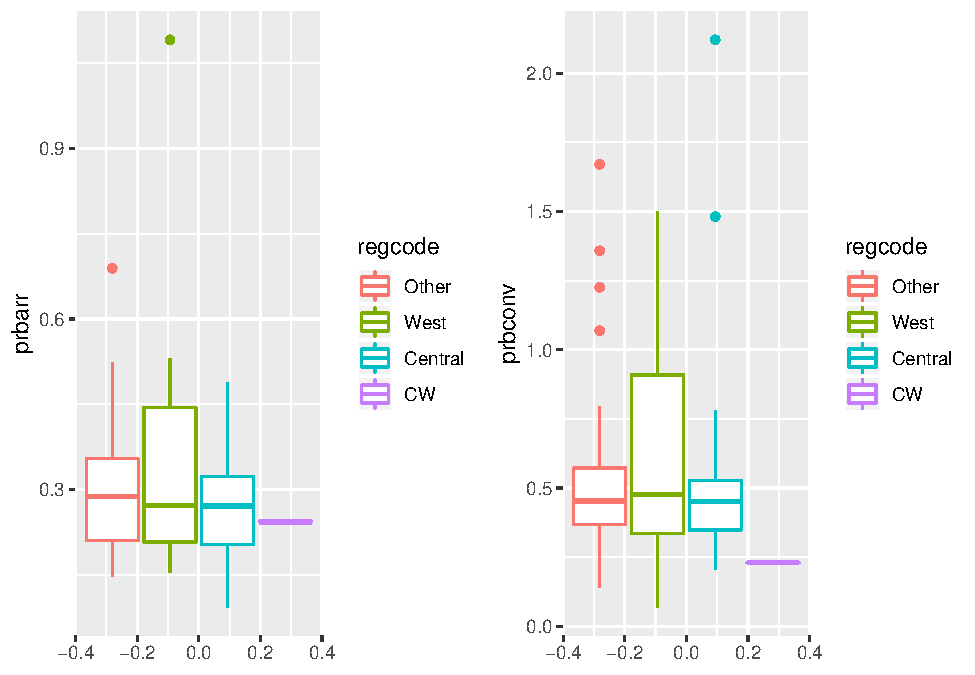
\includegraphics{Bagnard_Gaustad_Hartman_Leung_Lab_3_files/figure-latex/unnamed-chunk-22-1.pdf}

The criminal justice and law enforcement variables also show evidence of
possible outliers, notably, pbarr and polpc appear to have extreme data
points

We also see that prbarr and prbconv have values greater than 1. However,
these are not true probabity numbers and are instead ratios used as a
stand in for the true probability numbers.

There is a possibility of higher arrests per incident for an area.
Meaning, the area has low incidents in general but when there were
incidents there were also multiple arrests. The same case can be made
for the convictions per arrest variable which we see is for a different
region. In that county there may have been multiple charges brought per
one arrest.

\begin{Shaded}
\begin{Highlighting}[]
\CommentTok{#plot of demographic information for counties Outside and Inside the metro areas}
\CommentTok{# population density, percent minority, percent young male}

\NormalTok{q1<-}\KeywordTok{ggplot}\NormalTok{(}\DataTypeTok{data =}\NormalTok{ dfCrime, }\KeywordTok{aes}\NormalTok{(}\DataTypeTok{x =}\NormalTok{ density, }\DataTypeTok{y =}\NormalTok{ crmrte, }\DataTypeTok{color =}\NormalTok{ region)) }\OperatorTok{+}\StringTok{ }
\StringTok{      }\KeywordTok{geom_point}\NormalTok{() }\OperatorTok{+}\StringTok{ }\KeywordTok{facet_wrap}\NormalTok{(}\OperatorTok{~}\StringTok{ }\NormalTok{metro) }\OperatorTok{+}
\StringTok{  }\KeywordTok{geom_smooth}\NormalTok{(}\DataTypeTok{method =} \StringTok{"lm"}\NormalTok{)}
\NormalTok{q2<-}\KeywordTok{ggplot}\NormalTok{(}\DataTypeTok{data =}\NormalTok{ dfCrime, }\KeywordTok{aes}\NormalTok{(}\DataTypeTok{x =}\NormalTok{ pctmin80, }\DataTypeTok{y =}\NormalTok{ crmrte, }\DataTypeTok{color =}\NormalTok{ region)) }\OperatorTok{+}\StringTok{ }
\StringTok{      }\KeywordTok{geom_point}\NormalTok{() }\OperatorTok{+}\StringTok{ }\KeywordTok{facet_wrap}\NormalTok{(}\OperatorTok{~}\StringTok{ }\NormalTok{metro) }\OperatorTok{+}
\StringTok{  }\KeywordTok{geom_smooth}\NormalTok{(}\DataTypeTok{method =} \StringTok{"lm"}\NormalTok{)}
\NormalTok{q3<-}\KeywordTok{ggplot}\NormalTok{(}\DataTypeTok{data =}\NormalTok{ dfCrime, }\KeywordTok{aes}\NormalTok{(}\DataTypeTok{x =}\NormalTok{ pctymle, }\DataTypeTok{y =}\NormalTok{ crmrte, }\DataTypeTok{color =}\NormalTok{ region)) }\OperatorTok{+}\StringTok{ }
\StringTok{      }\KeywordTok{geom_point}\NormalTok{()}\OperatorTok{+}\StringTok{ }\KeywordTok{facet_wrap}\NormalTok{(}\OperatorTok{~}\StringTok{ }\NormalTok{metro) }\OperatorTok{+}
\StringTok{  }\KeywordTok{geom_smooth}\NormalTok{(}\DataTypeTok{method =} \StringTok{"lm"}\NormalTok{)}

\KeywordTok{grid.arrange}\NormalTok{(q1, q2, q3, }\DataTypeTok{ncol=}\DecValTok{1}\NormalTok{)}
\end{Highlighting}
\end{Shaded}

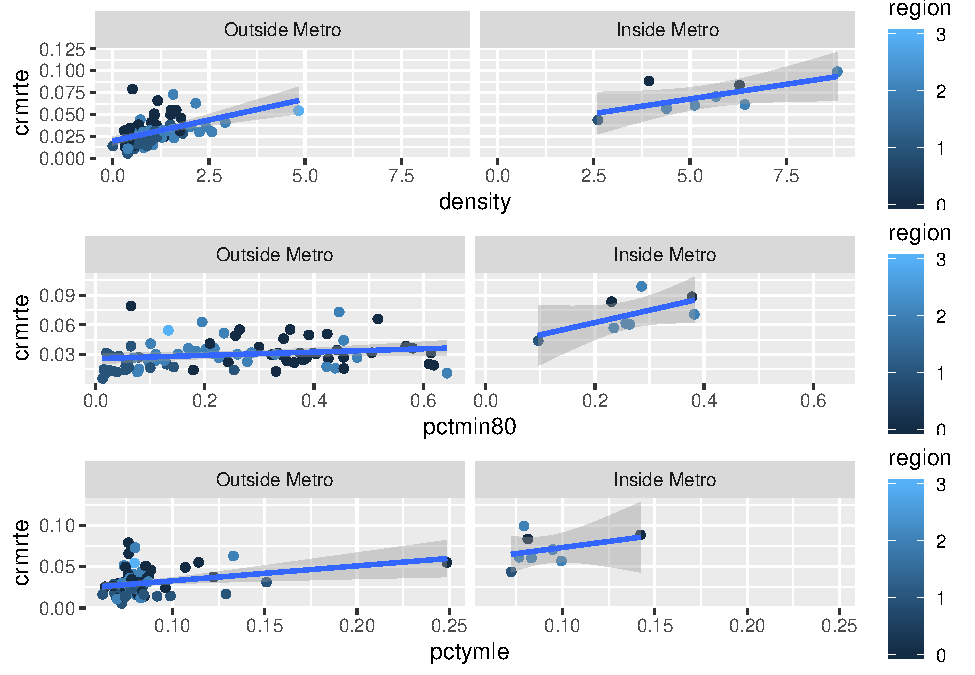
\includegraphics{Bagnard_Gaustad_Hartman_Leung_Lab_3_files/figure-latex/unnamed-chunk-23-1.pdf}

Notably more outliers are observed in demographic information. Here,
pctymle in one county outside of a metro area is nearly 25\%. That seems
quite high in normal statistical measures of the population, however,
this can be explained as a county having a large college town
population.

Finally, we can see our bright blue region 3 county and notice its
population density. Its behavior is more similar to an inside metro area
than outside. In addition to be coded for both western and central
regions, it appears to be miscoded here as well.

We will address the metro variable, and examine whether the region
variable should be west, central or other instead of both central and
west

\begin{Shaded}
\begin{Highlighting}[]
\NormalTok{dfCrime }\OperatorTok
\KeywordTok{filter}\NormalTok{(west }\OperatorTok{==}\DecValTok{1} \OperatorTok{&}\StringTok{ }\NormalTok{central }\OperatorTok{==}\DecValTok{1}\NormalTok{) }\OperatorTok
\KeywordTok{select}\NormalTok{(county, west, central, other, urban, region, regcode, metro)}
\end{Highlighting}
\end{Shaded}

\begin{verbatim}
  county west central other urban region regcode         metro
1     71    1       1     0     0      3      CW Outside Metro
\end{verbatim}

\begin{Shaded}
\begin{Highlighting}[]
\NormalTok{dfCrime}\OperatorTok{$}\NormalTok{west[}\KeywordTok{which}\NormalTok{(dfCrime}\OperatorTok{$}\NormalTok{county}\OperatorTok{==}\DecValTok{71}\NormalTok{)]<-}\OtherTok{NA}
\NormalTok{dfCrime}\OperatorTok{$}\NormalTok{central[}\KeywordTok{which}\NormalTok{(dfCrime}\OperatorTok{$}\NormalTok{county}\OperatorTok{==}\DecValTok{71}\NormalTok{)]<-}\OtherTok{NA}
\NormalTok{dfCrime}\OperatorTok{$}\NormalTok{other[}\KeywordTok{which}\NormalTok{(dfCrime}\OperatorTok{$}\NormalTok{county}\OperatorTok{==}\DecValTok{71}\NormalTok{)]<-}\OtherTok{NA}
\NormalTok{dfCrime}\OperatorTok{$}\NormalTok{urban[}\KeywordTok{which}\NormalTok{(dfCrime}\OperatorTok{$}\NormalTok{county}\OperatorTok{==}\DecValTok{71}\NormalTok{)]<-}\OtherTok{NA}
\end{Highlighting}
\end{Shaded}

\begin{Shaded}
\begin{Highlighting}[]
\NormalTok{impute_arg <-}\StringTok{ }\KeywordTok{aregImpute}\NormalTok{(}\OperatorTok{~}\StringTok{ }\NormalTok{crmrte }\OperatorTok{+}\StringTok{  }\NormalTok{urban }\OperatorTok{+}\StringTok{ }\NormalTok{central }\OperatorTok{+}\StringTok{ }\NormalTok{west }\OperatorTok{+}
\StringTok{                         }\NormalTok{prbarr }\OperatorTok{+}\StringTok{ }\NormalTok{prbconv }\OperatorTok{+}\StringTok{ }\NormalTok{prbpris }\OperatorTok{+}\StringTok{ }\NormalTok{avgsen }\OperatorTok{+}\StringTok{ }\NormalTok{polpc }\OperatorTok{+}\StringTok{ }
\StringTok{                         }\NormalTok{density }\OperatorTok{+}\StringTok{ }\NormalTok{taxpc }\OperatorTok{+}\StringTok{ }\NormalTok{pctmin80 }\OperatorTok{+}\StringTok{ }\NormalTok{wcon }\OperatorTok{+}\StringTok{ }\NormalTok{wtuc }\OperatorTok{+}
\StringTok{                         }\NormalTok{wtrd }\OperatorTok{+}\StringTok{ }\NormalTok{wfir }\OperatorTok{+}\StringTok{ }\NormalTok{wser }\OperatorTok{+}\StringTok{ }\NormalTok{wmfg }\OperatorTok{+}\StringTok{ }\NormalTok{wfed }\OperatorTok{+}\StringTok{ }\NormalTok{wsta }\OperatorTok{+}\StringTok{ }\NormalTok{wloc }\OperatorTok{+}
\StringTok{                         }\NormalTok{mix }\OperatorTok{+}\StringTok{ }\NormalTok{pctymle, }\DataTypeTok{data =}\NormalTok{ dfCrime, }\DataTypeTok{match=}\StringTok{"weighted"}\NormalTok{,}
                         \DataTypeTok{nk=}\DecValTok{3}\NormalTok{, }\DataTypeTok{B=}\DecValTok{10}\NormalTok{, }\DataTypeTok{n.impute =} \DecValTok{100}\NormalTok{)}
\end{Highlighting}
\end{Shaded}

\begin{Shaded}
\begin{Highlighting}[]
\KeywordTok{paste}\NormalTok{(}\StringTok{"R-squares for Predicting Non-Missing Values for Each Variable"}\NormalTok{)}
\end{Highlighting}
\end{Shaded}

\begin{verbatim}
[1] "R-squares for Predicting Non-Missing Values for Each Variable"
\end{verbatim}

\begin{Shaded}
\begin{Highlighting}[]
\NormalTok{impute_arg}\OperatorTok{$}\NormalTok{rsq}
\end{Highlighting}
\end{Shaded}

\begin{verbatim}
    urban   central      west 
0.9759023 0.8769296 0.9824131 
\end{verbatim}

\begin{Shaded}
\begin{Highlighting}[]
\KeywordTok{paste}\NormalTok{(}\StringTok{"Distribution of Values for Each Imputation"}\NormalTok{)}
\end{Highlighting}
\end{Shaded}

\begin{verbatim}
[1] "Distribution of Values for Each Imputation"
\end{verbatim}

\begin{Shaded}
\begin{Highlighting}[]
\KeywordTok{table}\NormalTok{(impute_arg}\OperatorTok{$}\NormalTok{imputed}\OperatorTok{$}\NormalTok{central)}
\end{Highlighting}
\end{Shaded}

\begin{verbatim}

 0  1 
33 67 
\end{verbatim}

\begin{Shaded}
\begin{Highlighting}[]
\KeywordTok{paste}\NormalTok{(}\StringTok{"Distribution of Values for Each Imputation"}\NormalTok{)}
\end{Highlighting}
\end{Shaded}

\begin{verbatim}
[1] "Distribution of Values for Each Imputation"
\end{verbatim}

\begin{Shaded}
\begin{Highlighting}[]
\KeywordTok{table}\NormalTok{(impute_arg}\OperatorTok{$}\NormalTok{imputed}\OperatorTok{$}\NormalTok{west)}
\end{Highlighting}
\end{Shaded}

\begin{verbatim}

 0  1 
78 22 
\end{verbatim}

\begin{Shaded}
\begin{Highlighting}[]
\KeywordTok{paste}\NormalTok{(}\StringTok{"Distribution of Values for Each Imputation"}\NormalTok{)}
\end{Highlighting}
\end{Shaded}

\begin{verbatim}
[1] "Distribution of Values for Each Imputation"
\end{verbatim}

\begin{Shaded}
\begin{Highlighting}[]
\KeywordTok{table}\NormalTok{(impute_arg}\OperatorTok{$}\NormalTok{imputed}\OperatorTok{$}\NormalTok{urban)}
\end{Highlighting}
\end{Shaded}

\begin{verbatim}

 0  1 
 9 91 
\end{verbatim}

The results confirm the county is urban. It is also highly probable that
county 71 is not west and most likely associated with central. After
correcting our data for urban and west, let's compare `central' with
`other' to be certain we have the right region.

\begin{Shaded}
\begin{Highlighting}[]
\CommentTok{#We need a mode function, so lets define one. Source - public domain}
\NormalTok{Mode =}\StringTok{ }\ControlFlowTok{function}\NormalTok{(x)\{ }
\NormalTok{    ta =}\StringTok{ }\KeywordTok{table}\NormalTok{(x)}
\NormalTok{    tam =}\StringTok{ }\KeywordTok{max}\NormalTok{(ta)}
    \ControlFlowTok{if}\NormalTok{ (}\KeywordTok{all}\NormalTok{(ta }\OperatorTok{==}\StringTok{ }\NormalTok{tam))}
\NormalTok{         mod =}\StringTok{ }\OtherTok{NA}
    \ControlFlowTok{else}
         \ControlFlowTok{if}\NormalTok{(}\KeywordTok{is.numeric}\NormalTok{(x))}
\NormalTok{    mod =}\StringTok{ }\KeywordTok{as.numeric}\NormalTok{(}\KeywordTok{names}\NormalTok{(ta)[ta }\OperatorTok{==}\StringTok{ }\NormalTok{tam])}
    \ControlFlowTok{else}
\NormalTok{         mod =}\StringTok{ }\KeywordTok{names}\NormalTok{(ta)[ta }\OperatorTok{==}\StringTok{ }\NormalTok{tam]}
    \KeywordTok{return}\NormalTok{(mod)}
\NormalTok{\}}

\NormalTok{dfCrime}\OperatorTok{$}\NormalTok{urban[}\KeywordTok{which}\NormalTok{(dfCrime}\OperatorTok{$}\NormalTok{county}\OperatorTok{==}\DecValTok{71}\NormalTok{)]<-}\KeywordTok{Mode}\NormalTok{(impute_arg}\OperatorTok{$}\NormalTok{imputed}\OperatorTok{$}\NormalTok{urban)}
\KeywordTok{print}\NormalTok{(}\StringTok{"Newly Reassigned urban Value for County 71:"}\NormalTok{)}
\end{Highlighting}
\end{Shaded}

\begin{verbatim}
[1] "Newly Reassigned urban Value for County 71:"
\end{verbatim}

\begin{Shaded}
\begin{Highlighting}[]
\NormalTok{dfCrime}\OperatorTok{$}\NormalTok{urban[}\KeywordTok{which}\NormalTok{(dfCrime}\OperatorTok{$}\NormalTok{county}\OperatorTok{==}\DecValTok{71}\NormalTok{)]}
\end{Highlighting}
\end{Shaded}

\begin{verbatim}
[1] 1
\end{verbatim}

\begin{Shaded}
\begin{Highlighting}[]
\NormalTok{dfCrime}\OperatorTok{$}\NormalTok{nonurban[}\KeywordTok{which}\NormalTok{(dfCrime}\OperatorTok{$}\NormalTok{county}\OperatorTok{==}\DecValTok{71}\NormalTok{)]<-}\DecValTok{1}\OperatorTok{-}\KeywordTok{Mode}\NormalTok{(impute_arg}\OperatorTok{$}\NormalTok{imputed}\OperatorTok{$}\NormalTok{urban)}
\KeywordTok{print}\NormalTok{(}\StringTok{"Newly Reassigned nonurban Value for County 71:"}\NormalTok{)}
\end{Highlighting}
\end{Shaded}

\begin{verbatim}
[1] "Newly Reassigned nonurban Value for County 71:"
\end{verbatim}

\begin{Shaded}
\begin{Highlighting}[]
\NormalTok{dfCrime}\OperatorTok{$}\NormalTok{nonurban[}\KeywordTok{which}\NormalTok{(dfCrime}\OperatorTok{$}\NormalTok{county}\OperatorTok{==}\DecValTok{71}\NormalTok{)]}
\end{Highlighting}
\end{Shaded}

\begin{verbatim}
[1] 0
\end{verbatim}

\begin{Shaded}
\begin{Highlighting}[]
\NormalTok{dfCrime}\OperatorTok{$}\NormalTok{west[}\KeywordTok{which}\NormalTok{(dfCrime}\OperatorTok{$}\NormalTok{county}\OperatorTok{==}\DecValTok{71}\NormalTok{)]<-}\KeywordTok{Mode}\NormalTok{(impute_arg}\OperatorTok{$}\NormalTok{imputed}\OperatorTok{$}\NormalTok{west)}
\KeywordTok{print}\NormalTok{(}\StringTok{"Newly Reassigned west Value for County 71:"}\NormalTok{)}
\end{Highlighting}
\end{Shaded}

\begin{verbatim}
[1] "Newly Reassigned west Value for County 71:"
\end{verbatim}

\begin{Shaded}
\begin{Highlighting}[]
\NormalTok{dfCrime}\OperatorTok{$}\NormalTok{west[}\KeywordTok{which}\NormalTok{(dfCrime}\OperatorTok{$}\NormalTok{county}\OperatorTok{==}\DecValTok{71}\NormalTok{)]}
\end{Highlighting}
\end{Shaded}

\begin{verbatim}
[1] 0
\end{verbatim}

\begin{Shaded}
\begin{Highlighting}[]
\NormalTok{impute_arg <-}\StringTok{ }\KeywordTok{aregImpute}\NormalTok{(}\OperatorTok{~}\StringTok{ }\NormalTok{crmrte }\OperatorTok{+}\StringTok{ }\NormalTok{central }\OperatorTok{+}\StringTok{ }\NormalTok{other }\OperatorTok{+}
\StringTok{                         }\NormalTok{prbarr }\OperatorTok{+}\StringTok{ }\NormalTok{prbconv }\OperatorTok{+}\StringTok{ }\NormalTok{prbpris }\OperatorTok{+}\StringTok{ }\NormalTok{avgsen }\OperatorTok{+}\StringTok{ }\NormalTok{polpc }\OperatorTok{+}\StringTok{ }
\StringTok{                         }\NormalTok{density }\OperatorTok{+}\StringTok{ }\NormalTok{taxpc }\OperatorTok{+}\StringTok{ }\NormalTok{pctmin80 }\OperatorTok{+}\StringTok{ }\NormalTok{wcon }\OperatorTok{+}\StringTok{ }\NormalTok{wtuc }\OperatorTok{+}
\StringTok{                         }\NormalTok{wtrd }\OperatorTok{+}\StringTok{ }\NormalTok{wfir }\OperatorTok{+}\StringTok{ }\NormalTok{wser }\OperatorTok{+}\StringTok{ }\NormalTok{wmfg }\OperatorTok{+}\StringTok{ }\NormalTok{wfed }\OperatorTok{+}\StringTok{ }\NormalTok{wsta }\OperatorTok{+}\StringTok{ }\NormalTok{wloc }\OperatorTok{+}
\StringTok{                         }\NormalTok{mix }\OperatorTok{+}\StringTok{ }\NormalTok{pctymle, }\DataTypeTok{data =}\NormalTok{ dfCrime, }\DataTypeTok{match=}\StringTok{"weighted"}\NormalTok{,}
                         \DataTypeTok{nk=}\DecValTok{3}\NormalTok{, }\DataTypeTok{B=}\DecValTok{10}\NormalTok{, }\DataTypeTok{n.impute =} \DecValTok{100}\NormalTok{)}
\end{Highlighting}
\end{Shaded}

\begin{Shaded}
\begin{Highlighting}[]
\KeywordTok{paste}\NormalTok{(}\StringTok{"R-squares for Predicting Non-Missing Values for Each Variable"}\NormalTok{)}
\end{Highlighting}
\end{Shaded}

\begin{verbatim}
[1] "R-squares for Predicting Non-Missing Values for Each Variable"
\end{verbatim}

\begin{Shaded}
\begin{Highlighting}[]
\NormalTok{impute_arg}\OperatorTok{$}\NormalTok{rsq}
\end{Highlighting}
\end{Shaded}

\begin{verbatim}
  central     other 
0.9147736 0.9050807 
\end{verbatim}

\begin{Shaded}
\begin{Highlighting}[]
\KeywordTok{paste}\NormalTok{(}\StringTok{"Distribution of Values for Each Imputation"}\NormalTok{)}
\end{Highlighting}
\end{Shaded}

\begin{verbatim}
[1] "Distribution of Values for Each Imputation"
\end{verbatim}

\begin{Shaded}
\begin{Highlighting}[]
\KeywordTok{table}\NormalTok{(impute_arg}\OperatorTok{$}\NormalTok{imputed}\OperatorTok{$}\NormalTok{other)}
\end{Highlighting}
\end{Shaded}

\begin{verbatim}

 0  1 
91  9 
\end{verbatim}

\begin{Shaded}
\begin{Highlighting}[]
\KeywordTok{paste}\NormalTok{(}\StringTok{"Distribution of Values for Each Imputation"}\NormalTok{)}
\end{Highlighting}
\end{Shaded}

\begin{verbatim}
[1] "Distribution of Values for Each Imputation"
\end{verbatim}

\begin{Shaded}
\begin{Highlighting}[]
\KeywordTok{table}\NormalTok{(impute_arg}\OperatorTok{$}\NormalTok{imputed}\OperatorTok{$}\NormalTok{central)}
\end{Highlighting}
\end{Shaded}

\begin{verbatim}

 0  1 
24 76 
\end{verbatim}

We also show a strong likelihood of the county not being other. The case
for central is high. Since the county is not western and not other it
must be in central by default, and the Hmisc algorithm bolsters that
suggestion. We'll assign our new values.

\begin{Shaded}
\begin{Highlighting}[]
\NormalTok{dfCrime}\OperatorTok{$}\NormalTok{other[}\KeywordTok{which}\NormalTok{(dfCrime}\OperatorTok{$}\NormalTok{county}\OperatorTok{==}\DecValTok{71}\NormalTok{)]<-}\KeywordTok{Mode}\NormalTok{(impute_arg}\OperatorTok{$}\NormalTok{imputed}\OperatorTok{$}\NormalTok{other)}
\NormalTok{dfCrime}\OperatorTok{$}\NormalTok{other[}\KeywordTok{which}\NormalTok{(dfCrime}\OperatorTok{$}\NormalTok{county}\OperatorTok{==}\DecValTok{71}\NormalTok{)]}
\end{Highlighting}
\end{Shaded}

\begin{verbatim}
[1] 0
\end{verbatim}

\begin{Shaded}
\begin{Highlighting}[]
\NormalTok{dfCrime}\OperatorTok{$}\NormalTok{central[}\KeywordTok{which}\NormalTok{(dfCrime}\OperatorTok{$}\NormalTok{county}\OperatorTok{==}\DecValTok{71}\NormalTok{)]<-}\DecValTok{1}\OperatorTok{-}\KeywordTok{Mode}\NormalTok{(impute_arg}\OperatorTok{$}\NormalTok{imputed}\OperatorTok{$}\NormalTok{other)}
\NormalTok{dfCrime}\OperatorTok{$}\NormalTok{central[}\KeywordTok{which}\NormalTok{(dfCrime}\OperatorTok{$}\NormalTok{county}\OperatorTok{==}\DecValTok{71}\NormalTok{)]}
\end{Highlighting}
\end{Shaded}

\begin{verbatim}
[1] 1
\end{verbatim}

Recode the categories for region and metro

\begin{Shaded}
\begin{Highlighting}[]
\NormalTok{dfCrime}\OperatorTok{$}\NormalTok{region <-}\StringTok{ }\KeywordTok{case_when}\NormalTok{ (}
\NormalTok{            (dfCrime}\OperatorTok{$}\NormalTok{central }\OperatorTok{==}\DecValTok{0} \OperatorTok{&}\StringTok{ }\NormalTok{dfCrime}\OperatorTok{$}\NormalTok{west }\OperatorTok{==}\DecValTok{0}\NormalTok{) }\OperatorTok{~}\StringTok{ }\DecValTok{0}\NormalTok{, }\CommentTok{#Eastern, Coastal, Other}
\NormalTok{            (dfCrime}\OperatorTok{$}\NormalTok{central }\OperatorTok{==}\DecValTok{0} \OperatorTok{&}\StringTok{ }\NormalTok{dfCrime}\OperatorTok{$}\NormalTok{west }\OperatorTok{==}\DecValTok{1}\NormalTok{) }\OperatorTok{~}\StringTok{ }\DecValTok{1}\NormalTok{, }\CommentTok{#Western}
\NormalTok{            (dfCrime}\OperatorTok{$}\NormalTok{central }\OperatorTok{==}\DecValTok{1} \OperatorTok{&}\StringTok{ }\NormalTok{dfCrime}\OperatorTok{$}\NormalTok{west }\OperatorTok{==}\DecValTok{0}\NormalTok{) }\OperatorTok{~}\StringTok{ }\DecValTok{2}  \CommentTok{#Central}
\NormalTok{        )}
\NormalTok{dfCrime}\OperatorTok{$}\NormalTok{regcode =}
\StringTok{            }\KeywordTok{factor}\NormalTok{( dfCrime}\OperatorTok{$}\NormalTok{region , }\DataTypeTok{levels =} \DecValTok{0}\OperatorTok{:}\DecValTok{2}\NormalTok{ , }\DataTypeTok{labels =}
                    \KeywordTok{c}\NormalTok{( }\StringTok{'Coastal'}\NormalTok{,}
                       \StringTok{'West'}\NormalTok{,}
                       \StringTok{'Central'}\NormalTok{ )}
\NormalTok{                   )}
\end{Highlighting}
\end{Shaded}

\begin{Shaded}
\begin{Highlighting}[]
\NormalTok{dfCrime}\OperatorTok{$}\NormalTok{metro =}
\StringTok{            }\KeywordTok{factor}\NormalTok{( dfCrime}\OperatorTok{$}\NormalTok{urban , }\DataTypeTok{levels =} \DecValTok{0}\OperatorTok{:}\DecValTok{1}\NormalTok{ , }\DataTypeTok{labels =}
                    \KeywordTok{c}\NormalTok{( }\StringTok{'Outside Metro'}\NormalTok{,}
                       \StringTok{'Inside Metro'}
\NormalTok{                      )}
\NormalTok{                   )}
\end{Highlighting}
\end{Shaded}

\begin{Shaded}
\begin{Highlighting}[]
\NormalTok{dfCrime }\OperatorTok
\KeywordTok{filter}\NormalTok{(county }\OperatorTok{==}\StringTok{ }\DecValTok{71}\NormalTok{) }\OperatorTok
\KeywordTok{select}\NormalTok{(county, west, central, urban, region, regcode, metro)}
\end{Highlighting}
\end{Shaded}

\begin{verbatim}
  county west central urban region regcode        metro
1     71    0       1     1      2 Central Inside Metro
\end{verbatim}

Let's review our density numbers again by looking in more detail at its
distribution.

\begin{Shaded}
\begin{Highlighting}[]
\KeywordTok{options}\NormalTok{(}\DataTypeTok{repr.plot.width=}\DecValTok{8}\NormalTok{, }\DataTypeTok{repr.plot.height=}\DecValTok{4}\NormalTok{)}
\KeywordTok{ggplot}\NormalTok{(}\DataTypeTok{data =}\NormalTok{ dfCrime, }\KeywordTok{aes}\NormalTok{(}\DataTypeTok{x =}\NormalTok{ density)) }\OperatorTok{+}\StringTok{ }
\StringTok{      }\KeywordTok{geom_histogram}\NormalTok{(}\DataTypeTok{bins=}\DecValTok{90}\NormalTok{)}
\end{Highlighting}
\end{Shaded}

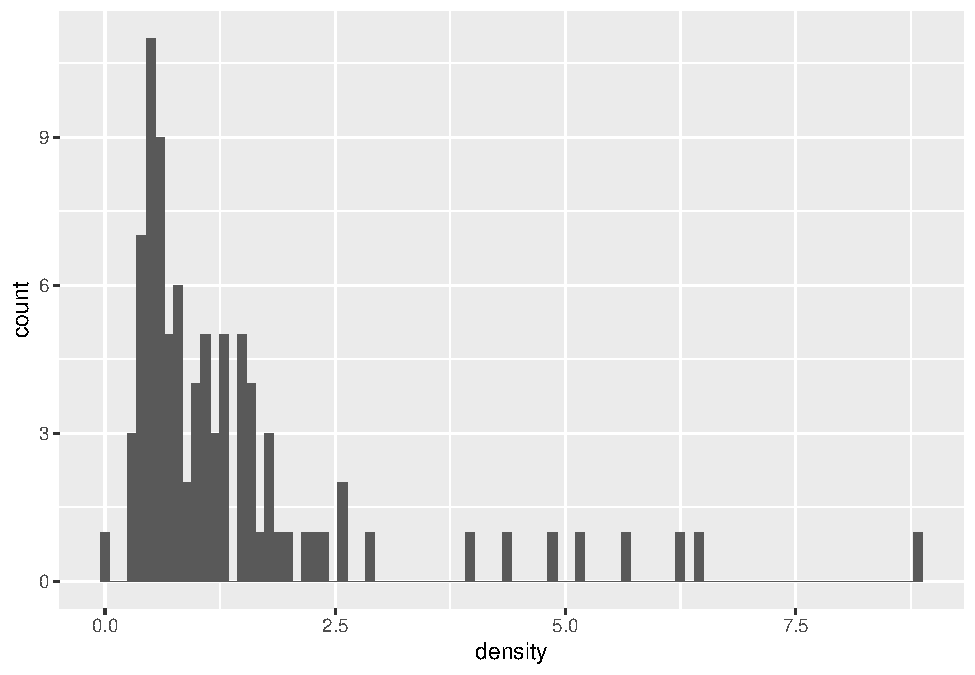
\includegraphics{Bagnard_Gaustad_Hartman_Leung_Lab_3_files/figure-latex/unnamed-chunk-40-1.pdf}

We note that one of the counties has an extremely low density. Near
zero.

\begin{Shaded}
\begin{Highlighting}[]
\NormalTok{dfCrime }\OperatorTok
\KeywordTok{filter}\NormalTok{(density }\OperatorTok{<}\StringTok{ }\FloatTok{0.01}\NormalTok{)}
\end{Highlighting}
\end{Shaded}

\begin{verbatim}
  county year    crmrte   prbarr  prbconv prbpris avgsen      polpc
1    173   87 0.0139937 0.530435 0.327869    0.15   6.64 0.00316379
      density    taxpc west central urban pctmin80    wcon     wtuc
1 2.03422e-05 37.72702    1       0     0 0.253914 231.696 213.6752
      wtrd    wfir     wser   wmfg   wfed   wsta   wloc       mix
1 175.1604 267.094 204.3792 193.01 334.44 414.68 304.32 0.4197531
     pctymle region regcode other nonurban         metro
1 0.07462687      1    West     0        1 Outside Metro
\end{verbatim}

In review of the North Carolina county density data from 1985, the
smallest population density in any county in North Carolina is 0.0952.
This makes the density of 0.0000203422 (ie. average of
\textasciitilde{}2.0 people per 10,000 square miles) for county 173
statistically impossible. It is miscoded.

\url{http://ncosbm.s3.amazonaws.com/s3fs-public/demog/dens7095.xls}

(Note to team: We could use this table if we want to assign names to our
counties by comparing the population densities. What is interesting is
that the 6 rows of missing values we removed earlier can be found in the
tail of this table. There was an arbitrary cut off after a certain
density - lkely because the counties were not statistically significant.
County 173 is not one of those counties, however, as our imputation
process will demonstrate.)

\begin{Shaded}
\begin{Highlighting}[]
\NormalTok{dfCrime}\OperatorTok{$}\NormalTok{density[}\KeywordTok{which}\NormalTok{(dfCrime}\OperatorTok{$}\NormalTok{county}\OperatorTok{==}\DecValTok{173}\NormalTok{)]<-}\StringTok{ }\OtherTok{NA}
\end{Highlighting}
\end{Shaded}

\begin{Shaded}
\begin{Highlighting}[]
\CommentTok{#dfSubset <-  we will use the non-urban western counties}
\NormalTok{impute_arg <-}\StringTok{ }\KeywordTok{aregImpute}\NormalTok{(}\OperatorTok{~}\StringTok{ }\NormalTok{crmrte }\OperatorTok{+}\StringTok{ }
\StringTok{                         }\NormalTok{prbarr }\OperatorTok{+}\StringTok{ }\NormalTok{prbconv }\OperatorTok{+}\StringTok{ }\NormalTok{prbpris }\OperatorTok{+}\StringTok{ }\NormalTok{avgsen }\OperatorTok{+}\StringTok{ }\NormalTok{polpc }\OperatorTok{+}\StringTok{ }
\StringTok{                         }\NormalTok{density }\OperatorTok{+}\StringTok{ }\NormalTok{taxpc }\OperatorTok{+}\StringTok{ }\NormalTok{pctmin80 }\OperatorTok{+}\StringTok{ }\NormalTok{wcon }\OperatorTok{+}\StringTok{ }\NormalTok{wtuc }\OperatorTok{+}
\StringTok{                         }\NormalTok{wtrd }\OperatorTok{+}\StringTok{ }\NormalTok{wfir }\OperatorTok{+}\StringTok{ }\NormalTok{wser }\OperatorTok{+}\StringTok{ }\NormalTok{wmfg }\OperatorTok{+}\StringTok{ }\NormalTok{wfed }\OperatorTok{+}\StringTok{ }\NormalTok{wsta }\OperatorTok{+}\StringTok{ }\NormalTok{wloc }\OperatorTok{+}
\StringTok{                         }\NormalTok{mix }\OperatorTok{+}\StringTok{ }\NormalTok{pctymle, }\DataTypeTok{data =}\NormalTok{ dfCrime }\OperatorTok\StringTok{ }\KeywordTok{filter}\NormalTok{(urban}\OperatorTok{==}\DecValTok{0} \OperatorTok{&}\StringTok{ }\NormalTok{west }\OperatorTok{==}\DecValTok{1}\NormalTok{),}
                         \DataTypeTok{match=}\StringTok{"weighted"}\NormalTok{,  }\DataTypeTok{nk=}\DecValTok{3}\NormalTok{, }\DataTypeTok{B=}\DecValTok{10}\NormalTok{, }\DataTypeTok{n.impute =} \DecValTok{30}\NormalTok{)}
\end{Highlighting}
\end{Shaded}

\begin{Shaded}
\begin{Highlighting}[]
\KeywordTok{paste}\NormalTok{(}\StringTok{"R-squares for Predicting Non-Missing Values for Each Variable"}\NormalTok{)}
\end{Highlighting}
\end{Shaded}

\begin{verbatim}
[1] "R-squares for Predicting Non-Missing Values for Each Variable"
\end{verbatim}

\begin{Shaded}
\begin{Highlighting}[]
\NormalTok{impute_arg}\OperatorTok{$}\NormalTok{rsq}
\end{Highlighting}
\end{Shaded}

\begin{verbatim}
density 
      1 
\end{verbatim}

\begin{Shaded}
\begin{Highlighting}[]
\KeywordTok{paste}\NormalTok{(}\StringTok{"Distribution of Values for Each Imputation"}\NormalTok{)}
\end{Highlighting}
\end{Shaded}

\begin{verbatim}
[1] "Distribution of Values for Each Imputation"
\end{verbatim}

\begin{Shaded}
\begin{Highlighting}[]
\KeywordTok{table}\NormalTok{(impute_arg}\OperatorTok{$}\NormalTok{imputed}\OperatorTok{$}\NormalTok{density)}
\end{Highlighting}
\end{Shaded}

\begin{verbatim}

0.385809302  0.41276595 0.864864886 0.889880955 1.498938441 1.815508008 
          1          20           2           1           2           4 
\end{verbatim}

\begin{Shaded}
\begin{Highlighting}[]
\NormalTok{dfCrime}\OperatorTok{$}\NormalTok{density[}\KeywordTok{which}\NormalTok{(dfCrime}\OperatorTok{$}\NormalTok{county}\OperatorTok{==}\DecValTok{173}\NormalTok{)]<-}\KeywordTok{mean}\NormalTok{(impute_arg}\OperatorTok{$}\NormalTok{imputed}\OperatorTok{$}\NormalTok{density)}
\NormalTok{dfCrime}\OperatorTok{$}\NormalTok{density[}\KeywordTok{which}\NormalTok{(dfCrime}\OperatorTok{$}\NormalTok{county}\OperatorTok{==}\DecValTok{173}\NormalTok{)]}
\end{Highlighting}
\end{Shaded}

\begin{verbatim}
[1] 0.7173549
\end{verbatim}

-- MOVE TO END OF PUT IN EACH MODEL -- Now, we will examine transforms
for better linearity.

\begin{Shaded}
\begin{Highlighting}[]
\CommentTok{#dfEconVars <- as.data.frame(cbind(dfCrime$wcon, dfCrime$wtuc, dfCrime$wtrd, dfCrime$wfir, }
\CommentTok{#                                  dfCrime$wser, dfCrime$wmfg, dfCrime$wfed, dfCrime$wsta, }
\CommentTok{#                                  dfCrime$wloc))}
\CommentTok{#names(dfEconVars) <- c('wcon', 'wtuc', 'wtrd', 'wfir', 'wser', }
\CommentTok{#                              'wmfg', 'wfed', 'wsta', 'wloc')}
\CommentTok{#}
\CommentTok{#ggplot(melt(dfEconVars),aes(x=value)) + geom_histogram(bins=30) + facet_wrap(~variable)}

\CommentTok{#The economic variables}
\NormalTok{q1<-}\KeywordTok{ggplot}\NormalTok{(}\DataTypeTok{data =}\NormalTok{ dfCrime, }\KeywordTok{aes}\NormalTok{(}\DataTypeTok{x =}\NormalTok{ wcon, }\DataTypeTok{y =}\NormalTok{ crmrte, }\DataTypeTok{color =}\NormalTok{ region)) }\OperatorTok{+}\StringTok{ }
\StringTok{      }\KeywordTok{geom_point}\NormalTok{()}\OperatorTok{+}
\StringTok{  }\KeywordTok{geom_smooth}\NormalTok{(}\DataTypeTok{method =} \StringTok{"lm"}\NormalTok{)}
\NormalTok{q1a<-}\KeywordTok{ggplot}\NormalTok{(}\DataTypeTok{data =}\NormalTok{ dfCrime, }\KeywordTok{aes}\NormalTok{(}\DataTypeTok{x =} \KeywordTok{log}\NormalTok{(wcon), }\DataTypeTok{y =} \KeywordTok{log}\NormalTok{(crmrte), }\DataTypeTok{color =}\NormalTok{ region)) }\OperatorTok{+}\StringTok{ }
\StringTok{      }\KeywordTok{geom_point}\NormalTok{()}\OperatorTok{+}
\StringTok{  }\KeywordTok{geom_smooth}\NormalTok{(}\DataTypeTok{method =} \StringTok{"lm"}\NormalTok{)}
\NormalTok{q2<-}\KeywordTok{ggplot}\NormalTok{(}\DataTypeTok{data =}\NormalTok{ dfCrime, }\KeywordTok{aes}\NormalTok{(}\DataTypeTok{x =}\NormalTok{ wtuc, }\DataTypeTok{y =}\NormalTok{ crmrte, }\DataTypeTok{color =}\NormalTok{ region)) }\OperatorTok{+}\StringTok{ }
\StringTok{      }\KeywordTok{geom_point}\NormalTok{()}\OperatorTok{+}
\StringTok{  }\KeywordTok{geom_smooth}\NormalTok{(}\DataTypeTok{method =} \StringTok{"lm"}\NormalTok{)}
\NormalTok{q2a<-}\KeywordTok{ggplot}\NormalTok{(}\DataTypeTok{data =}\NormalTok{ dfCrime, }\KeywordTok{aes}\NormalTok{(}\DataTypeTok{x =} \KeywordTok{log}\NormalTok{(wtuc), }\DataTypeTok{y =} \KeywordTok{log}\NormalTok{(crmrte), }\DataTypeTok{color =}\NormalTok{ region)) }\OperatorTok{+}\StringTok{ }
\StringTok{      }\KeywordTok{geom_point}\NormalTok{()}\OperatorTok{+}
\StringTok{  }\KeywordTok{geom_smooth}\NormalTok{(}\DataTypeTok{method =} \StringTok{"lm"}\NormalTok{)}
\NormalTok{q3<-}\KeywordTok{ggplot}\NormalTok{(}\DataTypeTok{data =}\NormalTok{ dfCrime, }\KeywordTok{aes}\NormalTok{(}\DataTypeTok{x =}\NormalTok{ wtrd, }\DataTypeTok{y =}\NormalTok{ crmrte, }\DataTypeTok{color =}\NormalTok{ region)) }\OperatorTok{+}\StringTok{ }
\StringTok{      }\KeywordTok{geom_point}\NormalTok{()}\OperatorTok{+}
\StringTok{  }\KeywordTok{geom_smooth}\NormalTok{(}\DataTypeTok{method =} \StringTok{"lm"}\NormalTok{)}
\NormalTok{q3a<-}\KeywordTok{ggplot}\NormalTok{(}\DataTypeTok{data =}\NormalTok{ dfCrime, }\KeywordTok{aes}\NormalTok{(}\DataTypeTok{x =} \KeywordTok{log}\NormalTok{(wtrd), }\DataTypeTok{y =} \KeywordTok{log}\NormalTok{(crmrte), }\DataTypeTok{color =}\NormalTok{ region)) }\OperatorTok{+}\StringTok{ }
\StringTok{      }\KeywordTok{geom_point}\NormalTok{()}\OperatorTok{+}
\StringTok{  }\KeywordTok{geom_smooth}\NormalTok{(}\DataTypeTok{method =} \StringTok{"lm"}\NormalTok{)}
\NormalTok{q4<-}\KeywordTok{ggplot}\NormalTok{(}\DataTypeTok{data =}\NormalTok{ dfCrime, }\KeywordTok{aes}\NormalTok{(}\DataTypeTok{x =}\NormalTok{ wfir, }\DataTypeTok{y =}\NormalTok{ crmrte, }\DataTypeTok{color =}\NormalTok{ region)) }\OperatorTok{+}\StringTok{ }
\StringTok{      }\KeywordTok{geom_point}\NormalTok{()}\OperatorTok{+}
\StringTok{  }\KeywordTok{geom_smooth}\NormalTok{(}\DataTypeTok{method =} \StringTok{"lm"}\NormalTok{)}
\NormalTok{q4a<-}\KeywordTok{ggplot}\NormalTok{(}\DataTypeTok{data =}\NormalTok{ dfCrime, }\KeywordTok{aes}\NormalTok{(}\DataTypeTok{x =} \KeywordTok{log}\NormalTok{(wfir), }\DataTypeTok{y =} \KeywordTok{log}\NormalTok{(crmrte), }\DataTypeTok{color =}\NormalTok{ region)) }\OperatorTok{+}\StringTok{ }
\StringTok{      }\KeywordTok{geom_point}\NormalTok{()}\OperatorTok{+}
\StringTok{  }\KeywordTok{geom_smooth}\NormalTok{(}\DataTypeTok{method =} \StringTok{"lm"}\NormalTok{)}
\NormalTok{q5<-}\KeywordTok{ggplot}\NormalTok{(}\DataTypeTok{data =}\NormalTok{ dfCrime, }\KeywordTok{aes}\NormalTok{(}\DataTypeTok{x =}\NormalTok{ wser, }\DataTypeTok{y =}\NormalTok{ crmrte, }\DataTypeTok{color =}\NormalTok{ region)) }\OperatorTok{+}\StringTok{ }
\StringTok{      }\KeywordTok{geom_point}\NormalTok{()}\OperatorTok{+}
\StringTok{  }\KeywordTok{geom_smooth}\NormalTok{(}\DataTypeTok{method =} \StringTok{"lm"}\NormalTok{)}
\NormalTok{q5a<-}\KeywordTok{ggplot}\NormalTok{(}\DataTypeTok{data =}\NormalTok{ dfCrime, }\KeywordTok{aes}\NormalTok{(}\DataTypeTok{x =} \KeywordTok{log}\NormalTok{(wser), }\DataTypeTok{y =} \KeywordTok{log}\NormalTok{(crmrte), }\DataTypeTok{color =}\NormalTok{ region)) }\OperatorTok{+}\StringTok{ }
\StringTok{      }\KeywordTok{geom_point}\NormalTok{()}\OperatorTok{+}
\StringTok{  }\KeywordTok{geom_smooth}\NormalTok{(}\DataTypeTok{method =} \StringTok{"lm"}\NormalTok{)}
\NormalTok{q6<-}\KeywordTok{ggplot}\NormalTok{(}\DataTypeTok{data =}\NormalTok{ dfCrime, }\KeywordTok{aes}\NormalTok{(}\DataTypeTok{x =}\NormalTok{ wmfg, }\DataTypeTok{y =}\NormalTok{ crmrte, }\DataTypeTok{color =}\NormalTok{ region)) }\OperatorTok{+}\StringTok{ }
\StringTok{      }\KeywordTok{geom_point}\NormalTok{()}\OperatorTok{+}
\StringTok{  }\KeywordTok{geom_smooth}\NormalTok{(}\DataTypeTok{method =} \StringTok{"lm"}\NormalTok{)}
\NormalTok{q6a<-}\KeywordTok{ggplot}\NormalTok{(}\DataTypeTok{data =}\NormalTok{ dfCrime, }\KeywordTok{aes}\NormalTok{(}\DataTypeTok{x =} \KeywordTok{log}\NormalTok{(wmfg), }\DataTypeTok{y =} \KeywordTok{log}\NormalTok{(crmrte), }\DataTypeTok{color =}\NormalTok{ region)) }\OperatorTok{+}\StringTok{ }
\StringTok{      }\KeywordTok{geom_point}\NormalTok{()}\OperatorTok{+}
\StringTok{  }\KeywordTok{geom_smooth}\NormalTok{(}\DataTypeTok{method =} \StringTok{"lm"}\NormalTok{)}
\NormalTok{q7<-}\KeywordTok{ggplot}\NormalTok{(}\DataTypeTok{data =}\NormalTok{ dfCrime, }\KeywordTok{aes}\NormalTok{(}\DataTypeTok{x =}\NormalTok{ wfed, }\DataTypeTok{y =}\NormalTok{ crmrte, }\DataTypeTok{color =}\NormalTok{ region)) }\OperatorTok{+}\StringTok{ }
\StringTok{      }\KeywordTok{geom_point}\NormalTok{()}\OperatorTok{+}
\StringTok{  }\KeywordTok{geom_smooth}\NormalTok{(}\DataTypeTok{method =} \StringTok{"lm"}\NormalTok{)}
\NormalTok{q7a<-}\KeywordTok{ggplot}\NormalTok{(}\DataTypeTok{data =}\NormalTok{ dfCrime, }\KeywordTok{aes}\NormalTok{(}\DataTypeTok{x =} \KeywordTok{log}\NormalTok{(wfed), }\DataTypeTok{y =} \KeywordTok{log}\NormalTok{(crmrte), }\DataTypeTok{color =}\NormalTok{ region)) }\OperatorTok{+}\StringTok{ }
\StringTok{      }\KeywordTok{geom_point}\NormalTok{()}\OperatorTok{+}
\StringTok{  }\KeywordTok{geom_smooth}\NormalTok{(}\DataTypeTok{method =} \StringTok{"lm"}\NormalTok{)}
\NormalTok{q8<-}\KeywordTok{ggplot}\NormalTok{(}\DataTypeTok{data =}\NormalTok{ dfCrime, }\KeywordTok{aes}\NormalTok{(}\DataTypeTok{x =}\NormalTok{ wsta, }\DataTypeTok{y =}\NormalTok{ crmrte, }\DataTypeTok{color =}\NormalTok{ region)) }\OperatorTok{+}\StringTok{ }
\StringTok{      }\KeywordTok{geom_point}\NormalTok{()}\OperatorTok{+}
\StringTok{  }\KeywordTok{geom_smooth}\NormalTok{(}\DataTypeTok{method =} \StringTok{"lm"}\NormalTok{)}
\NormalTok{q8a<-}\KeywordTok{ggplot}\NormalTok{(}\DataTypeTok{data =}\NormalTok{ dfCrime, }\KeywordTok{aes}\NormalTok{(}\DataTypeTok{x =} \KeywordTok{log}\NormalTok{(wsta), }\DataTypeTok{y =} \KeywordTok{log}\NormalTok{(crmrte), }\DataTypeTok{color =}\NormalTok{ region)) }\OperatorTok{+}\StringTok{ }
\StringTok{      }\KeywordTok{geom_point}\NormalTok{()}\OperatorTok{+}
\StringTok{  }\KeywordTok{geom_smooth}\NormalTok{(}\DataTypeTok{method =} \StringTok{"lm"}\NormalTok{)}
\NormalTok{q9<-}\KeywordTok{ggplot}\NormalTok{(}\DataTypeTok{data =}\NormalTok{ dfCrime, }\KeywordTok{aes}\NormalTok{(}\DataTypeTok{x =}\NormalTok{ wloc, }\DataTypeTok{y =}\NormalTok{ crmrte, }\DataTypeTok{color =}\NormalTok{ region)) }\OperatorTok{+}\StringTok{ }
\StringTok{      }\KeywordTok{geom_point}\NormalTok{()}\OperatorTok{+}
\StringTok{  }\KeywordTok{geom_smooth}\NormalTok{(}\DataTypeTok{method =} \StringTok{"lm"}\NormalTok{)}
\NormalTok{q9a<-}\KeywordTok{ggplot}\NormalTok{(}\DataTypeTok{data =}\NormalTok{ dfCrime, }\KeywordTok{aes}\NormalTok{(}\DataTypeTok{x =} \KeywordTok{log}\NormalTok{(wloc), }\DataTypeTok{y =} \KeywordTok{log}\NormalTok{(crmrte), }\DataTypeTok{color =}\NormalTok{ region)) }\OperatorTok{+}\StringTok{ }
\StringTok{      }\KeywordTok{geom_point}\NormalTok{()}\OperatorTok{+}
\StringTok{  }\KeywordTok{geom_smooth}\NormalTok{(}\DataTypeTok{method =} \StringTok{"lm"}\NormalTok{)}

\KeywordTok{options}\NormalTok{(}\DataTypeTok{repr.plot.width=}\DecValTok{8}\NormalTok{, }\DataTypeTok{repr.plot.height=}\DecValTok{16}\NormalTok{)}
\KeywordTok{grid.arrange}\NormalTok{(q1, q1a, q2, q2a, q3, q3a, }\DataTypeTok{ncol=}\DecValTok{2}\NormalTok{)}
\end{Highlighting}
\end{Shaded}

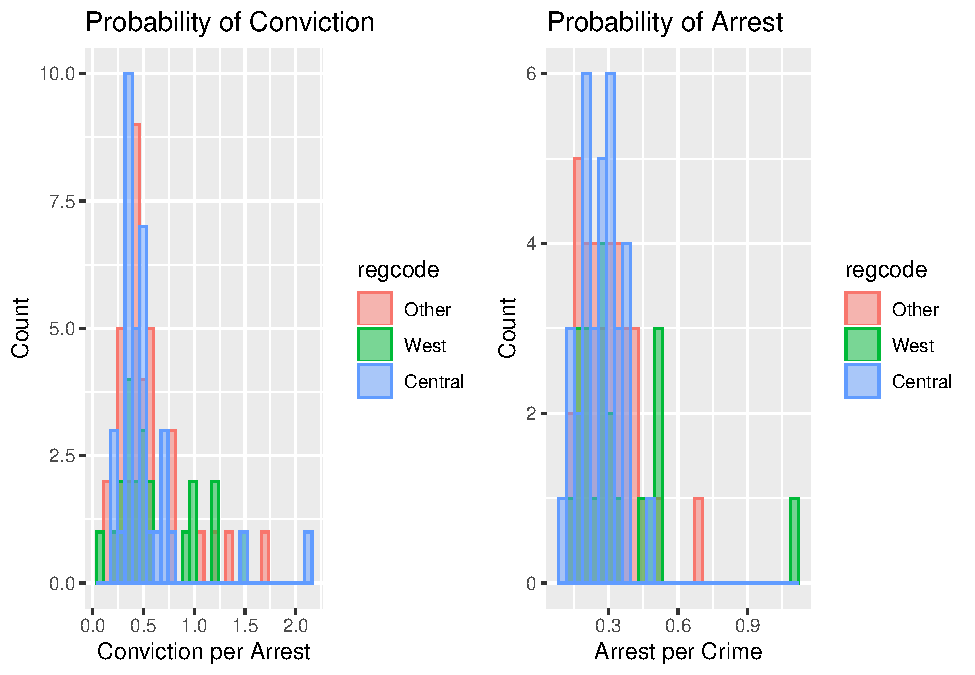
\includegraphics{Bagnard_Gaustad_Hartman_Leung_Lab_3_files/figure-latex/unnamed-chunk-47-1.pdf}

\begin{Shaded}
\begin{Highlighting}[]
\KeywordTok{grid.arrange}\NormalTok{(q4, q4a, q5, q5a, q6, q6a, }\DataTypeTok{ncol=}\DecValTok{2}\NormalTok{)}
\end{Highlighting}
\end{Shaded}

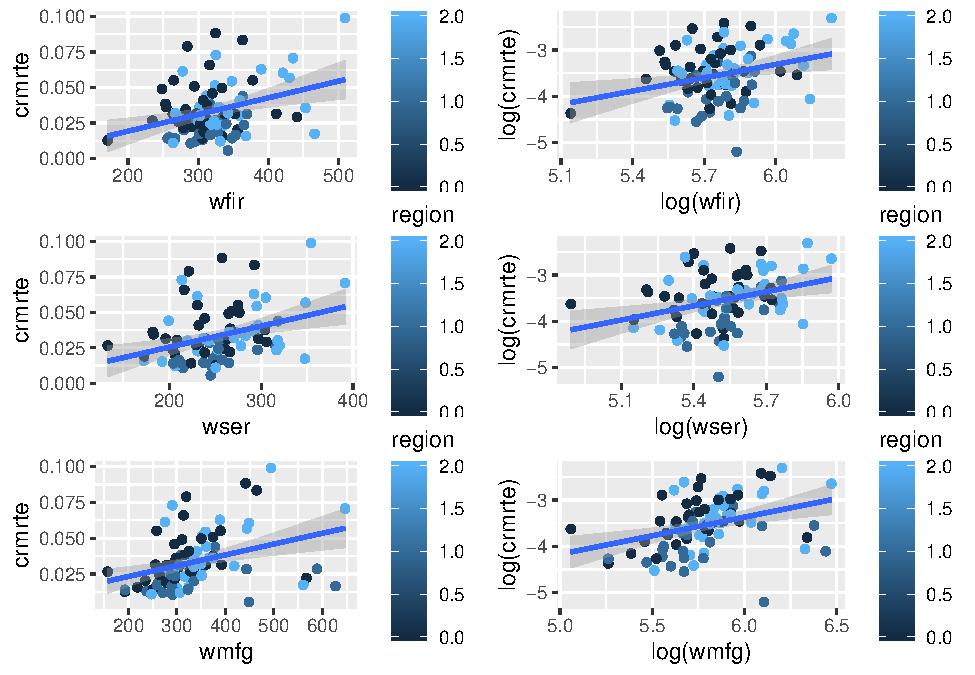
\includegraphics{Bagnard_Gaustad_Hartman_Leung_Lab_3_files/figure-latex/unnamed-chunk-47-2.pdf}

\begin{Shaded}
\begin{Highlighting}[]
\KeywordTok{grid.arrange}\NormalTok{(q7, q7a, q8, q8a, q9, q9a, }\DataTypeTok{ncol=}\DecValTok{2}\NormalTok{)}
\end{Highlighting}
\end{Shaded}

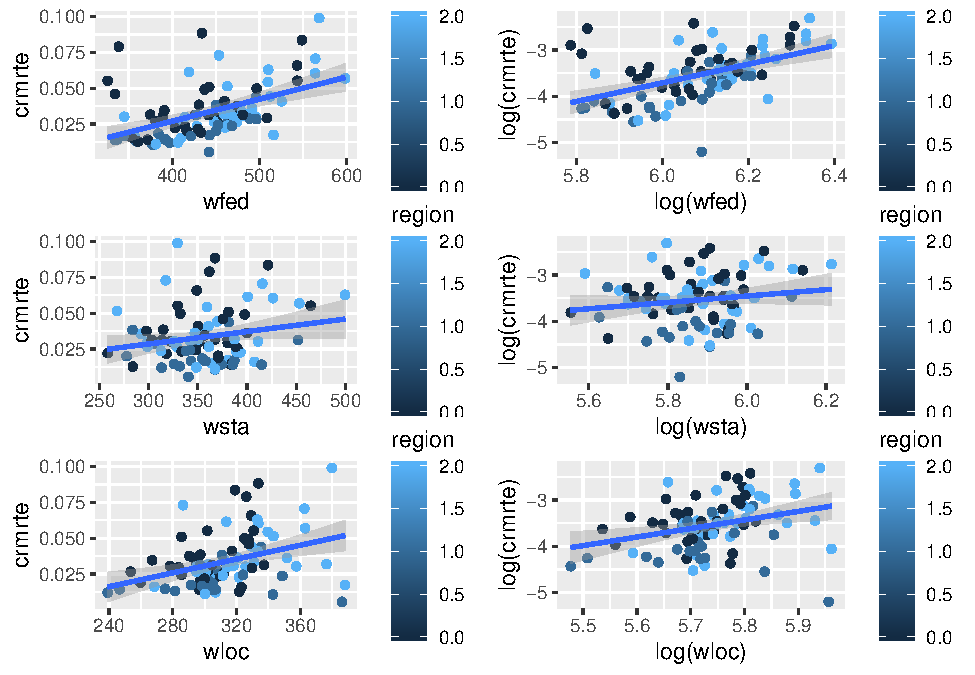
\includegraphics{Bagnard_Gaustad_Hartman_Leung_Lab_3_files/figure-latex/unnamed-chunk-47-3.pdf}

The transforms make the relationship more linearly distributed. We will
transform these variables to their log equivalents.

\begin{Shaded}
\begin{Highlighting}[]
\NormalTok{dfCrime}\OperatorTok{$}\NormalTok{logwcon<-}\KeywordTok{log}\NormalTok{(dfCrime}\OperatorTok{$}\NormalTok{wcon)}
\NormalTok{dfCrime}\OperatorTok{$}\NormalTok{logwtuc<-}\KeywordTok{log}\NormalTok{(dfCrime}\OperatorTok{$}\NormalTok{wtuc)}
\NormalTok{dfCrime}\OperatorTok{$}\NormalTok{logwtrd<-}\KeywordTok{log}\NormalTok{(dfCrime}\OperatorTok{$}\NormalTok{wtrd)}
\NormalTok{dfCrime}\OperatorTok{$}\NormalTok{logwfir<-}\KeywordTok{log}\NormalTok{(dfCrime}\OperatorTok{$}\NormalTok{wfir)}
\NormalTok{dfCrime}\OperatorTok{$}\NormalTok{logwser<-}\KeywordTok{log}\NormalTok{(dfCrime}\OperatorTok{$}\NormalTok{wser)}
\NormalTok{dfCrime}\OperatorTok{$}\NormalTok{logwmfg<-}\KeywordTok{log}\NormalTok{(dfCrime}\OperatorTok{$}\NormalTok{wmfg)}
\NormalTok{dfCrime}\OperatorTok{$}\NormalTok{logwfed<-}\KeywordTok{log}\NormalTok{(dfCrime}\OperatorTok{$}\NormalTok{wfed)}
\NormalTok{dfCrime}\OperatorTok{$}\NormalTok{logwsta<-}\KeywordTok{log}\NormalTok{(dfCrime}\OperatorTok{$}\NormalTok{wsta)}
\NormalTok{dfCrime}\OperatorTok{$}\NormalTok{logwloc<-}\KeywordTok{log}\NormalTok{(dfCrime}\OperatorTok{$}\NormalTok{wloc)}
\end{Highlighting}
\end{Shaded}

We move to the justice an law enforcement variables. With these
variables being mostly \textless{} 1 we'll also take the log for
comparison.

\begin{Shaded}
\begin{Highlighting}[]
\CommentTok{#Plot of the criminal justice and law enforcment related variables vs crmrte}
\NormalTok{q1<-}\KeywordTok{ggplot}\NormalTok{(}\DataTypeTok{data =}\NormalTok{ dfCrime, }\KeywordTok{aes}\NormalTok{(}\DataTypeTok{x =}\NormalTok{ prbarr, }\DataTypeTok{y =}\NormalTok{ crmrte, }\DataTypeTok{color =}\NormalTok{ region)) }\OperatorTok{+}\StringTok{ }
\StringTok{      }\KeywordTok{geom_point}\NormalTok{()}\OperatorTok{+}
\StringTok{  }\KeywordTok{geom_smooth}\NormalTok{(}\DataTypeTok{method =} \StringTok{"lm"}\NormalTok{)}
\NormalTok{q1a<-}\KeywordTok{ggplot}\NormalTok{(}\DataTypeTok{data =}\NormalTok{ dfCrime, }\KeywordTok{aes}\NormalTok{(}\DataTypeTok{x =} \KeywordTok{log}\NormalTok{(prbarr), }\DataTypeTok{y =} \KeywordTok{log}\NormalTok{(crmrte), }\DataTypeTok{color =}\NormalTok{ region)) }\OperatorTok{+}\StringTok{ }
\StringTok{      }\KeywordTok{geom_point}\NormalTok{()}\OperatorTok{+}
\StringTok{  }\KeywordTok{geom_smooth}\NormalTok{(}\DataTypeTok{method =} \StringTok{"lm"}\NormalTok{)}
\NormalTok{q2<-}\KeywordTok{ggplot}\NormalTok{(}\DataTypeTok{data =}\NormalTok{ dfCrime, }\KeywordTok{aes}\NormalTok{(}\DataTypeTok{x =}\NormalTok{ prbconv, }\DataTypeTok{y =}\NormalTok{ crmrte, }\DataTypeTok{color =}\NormalTok{ region)) }\OperatorTok{+}\StringTok{ }
\StringTok{      }\KeywordTok{geom_point}\NormalTok{()}\OperatorTok{+}
\StringTok{  }\KeywordTok{geom_smooth}\NormalTok{(}\DataTypeTok{method =} \StringTok{"lm"}\NormalTok{)}
\NormalTok{q2a<-}\KeywordTok{ggplot}\NormalTok{(}\DataTypeTok{data =}\NormalTok{ dfCrime, }\KeywordTok{aes}\NormalTok{(}\DataTypeTok{x =} \KeywordTok{log}\NormalTok{(prbconv), }\DataTypeTok{y =} \KeywordTok{log}\NormalTok{(crmrte), }\DataTypeTok{color =}\NormalTok{ region)) }\OperatorTok{+}\StringTok{ }
\StringTok{      }\KeywordTok{geom_point}\NormalTok{()}\OperatorTok{+}
\StringTok{  }\KeywordTok{geom_smooth}\NormalTok{(}\DataTypeTok{method =} \StringTok{"lm"}\NormalTok{)}
\NormalTok{q3<-}\KeywordTok{ggplot}\NormalTok{(}\DataTypeTok{data =}\NormalTok{ dfCrime, }\KeywordTok{aes}\NormalTok{(}\DataTypeTok{x =}\NormalTok{ prbpris, }\DataTypeTok{y =}\NormalTok{ crmrte, }\DataTypeTok{color =}\NormalTok{ region)) }\OperatorTok{+}\StringTok{ }
\StringTok{      }\KeywordTok{geom_point}\NormalTok{()}\OperatorTok{+}
\StringTok{  }\KeywordTok{geom_smooth}\NormalTok{(}\DataTypeTok{method =} \StringTok{"lm"}\NormalTok{)}
\NormalTok{q3a<-}\KeywordTok{ggplot}\NormalTok{(}\DataTypeTok{data =}\NormalTok{ dfCrime, }\KeywordTok{aes}\NormalTok{(}\DataTypeTok{x =} \KeywordTok{log}\NormalTok{(prbpris), }\DataTypeTok{y =} \KeywordTok{log}\NormalTok{(crmrte), }\DataTypeTok{color =}\NormalTok{ region)) }\OperatorTok{+}\StringTok{ }
\StringTok{      }\KeywordTok{geom_point}\NormalTok{()}\OperatorTok{+}
\StringTok{  }\KeywordTok{geom_smooth}\NormalTok{(}\DataTypeTok{method =} \StringTok{"lm"}\NormalTok{)}
\NormalTok{q4<-}\KeywordTok{ggplot}\NormalTok{(}\DataTypeTok{data =}\NormalTok{ dfCrime, }\KeywordTok{aes}\NormalTok{(}\DataTypeTok{x =}\NormalTok{ avgsen, }\DataTypeTok{y =}\NormalTok{ crmrte, }\DataTypeTok{color =}\NormalTok{ region)) }\OperatorTok{+}\StringTok{ }
\StringTok{      }\KeywordTok{geom_point}\NormalTok{()}\OperatorTok{+}
\StringTok{  }\KeywordTok{geom_smooth}\NormalTok{(}\DataTypeTok{method =} \StringTok{"lm"}\NormalTok{)}
\NormalTok{q4a<-}\KeywordTok{ggplot}\NormalTok{(}\DataTypeTok{data =}\NormalTok{ dfCrime, }\KeywordTok{aes}\NormalTok{(}\DataTypeTok{x =} \KeywordTok{log}\NormalTok{(avgsen), }\DataTypeTok{y =} \KeywordTok{log}\NormalTok{(crmrte), }\DataTypeTok{color =}\NormalTok{ region)) }\OperatorTok{+}\StringTok{ }
\StringTok{      }\KeywordTok{geom_point}\NormalTok{()}\OperatorTok{+}
\StringTok{  }\KeywordTok{geom_smooth}\NormalTok{(}\DataTypeTok{method =} \StringTok{"lm"}\NormalTok{)}
\NormalTok{q5<-}\KeywordTok{ggplot}\NormalTok{(}\DataTypeTok{data =}\NormalTok{ dfCrime, }\KeywordTok{aes}\NormalTok{(}\DataTypeTok{x =}\NormalTok{ polpc, }\DataTypeTok{y =}\NormalTok{ crmrte, }\DataTypeTok{color =}\NormalTok{ region)) }\OperatorTok{+}\StringTok{ }
\StringTok{      }\KeywordTok{geom_point}\NormalTok{()}\OperatorTok{+}
\StringTok{  }\KeywordTok{geom_smooth}\NormalTok{(}\DataTypeTok{method =} \StringTok{"lm"}\NormalTok{)}
\NormalTok{q5a<-}\KeywordTok{ggplot}\NormalTok{(}\DataTypeTok{data =}\NormalTok{ dfCrime, }\KeywordTok{aes}\NormalTok{(}\DataTypeTok{x =} \KeywordTok{log}\NormalTok{(polpc), }\DataTypeTok{y =} \KeywordTok{log}\NormalTok{(crmrte), }\DataTypeTok{color =}\NormalTok{ region)) }\OperatorTok{+}\StringTok{ }
\StringTok{      }\KeywordTok{geom_point}\NormalTok{()}\OperatorTok{+}
\StringTok{  }\KeywordTok{geom_smooth}\NormalTok{(}\DataTypeTok{method =} \StringTok{"lm"}\NormalTok{)}
\NormalTok{q6<-}\KeywordTok{ggplot}\NormalTok{(}\DataTypeTok{data =}\NormalTok{ dfCrime, }\KeywordTok{aes}\NormalTok{(}\DataTypeTok{x =}\NormalTok{ mix, }\DataTypeTok{y =}\NormalTok{ crmrte, }\DataTypeTok{color =}\NormalTok{ region)) }\OperatorTok{+}\StringTok{ }
\StringTok{      }\KeywordTok{geom_point}\NormalTok{()}\OperatorTok{+}
\StringTok{  }\KeywordTok{geom_smooth}\NormalTok{(}\DataTypeTok{method =} \StringTok{"lm"}\NormalTok{)}
\NormalTok{q6a<-}\KeywordTok{ggplot}\NormalTok{(}\DataTypeTok{data =}\NormalTok{ dfCrime, }\KeywordTok{aes}\NormalTok{(}\DataTypeTok{x =} \KeywordTok{log}\NormalTok{(mix), }\DataTypeTok{y =} \KeywordTok{log}\NormalTok{(crmrte), }\DataTypeTok{color =}\NormalTok{ region)) }\OperatorTok{+}\StringTok{ }
\StringTok{      }\KeywordTok{geom_point}\NormalTok{()}\OperatorTok{+}
\StringTok{  }\KeywordTok{geom_smooth}\NormalTok{(}\DataTypeTok{method =} \StringTok{"lm"}\NormalTok{)}

\KeywordTok{grid.arrange}\NormalTok{(q1, q1a, q2, q2a, q3, q3a, }\DataTypeTok{ncol=}\DecValTok{2}\NormalTok{)}
\end{Highlighting}
\end{Shaded}

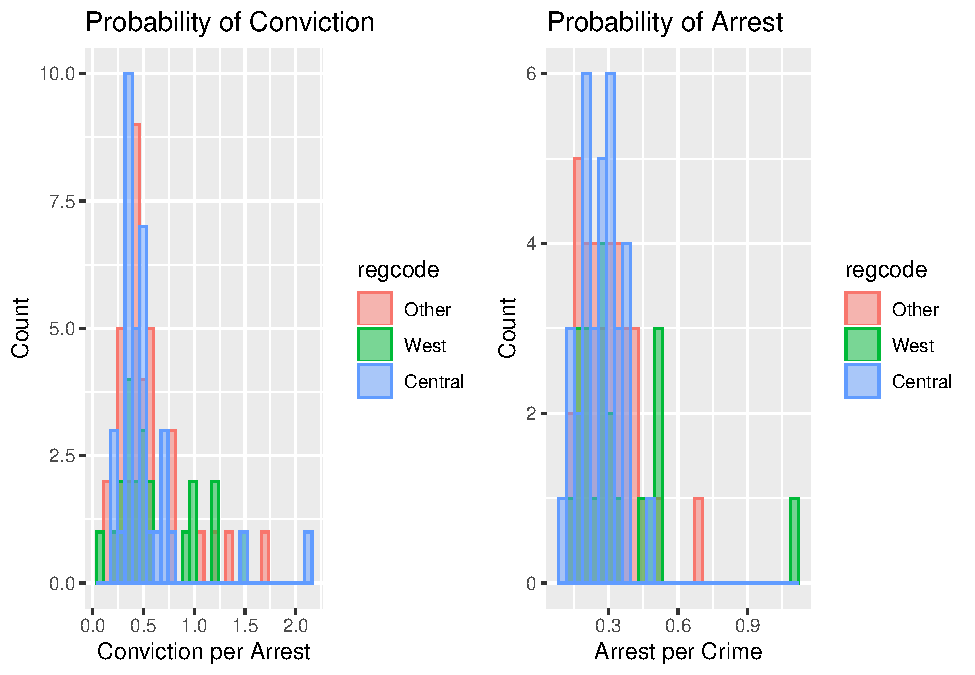
\includegraphics{Bagnard_Gaustad_Hartman_Leung_Lab_3_files/figure-latex/unnamed-chunk-49-1.pdf}

\begin{Shaded}
\begin{Highlighting}[]
\KeywordTok{grid.arrange}\NormalTok{(q4, q4a, q5, q5a, q6, q6a, }\DataTypeTok{ncol=}\DecValTok{2}\NormalTok{)}
\end{Highlighting}
\end{Shaded}

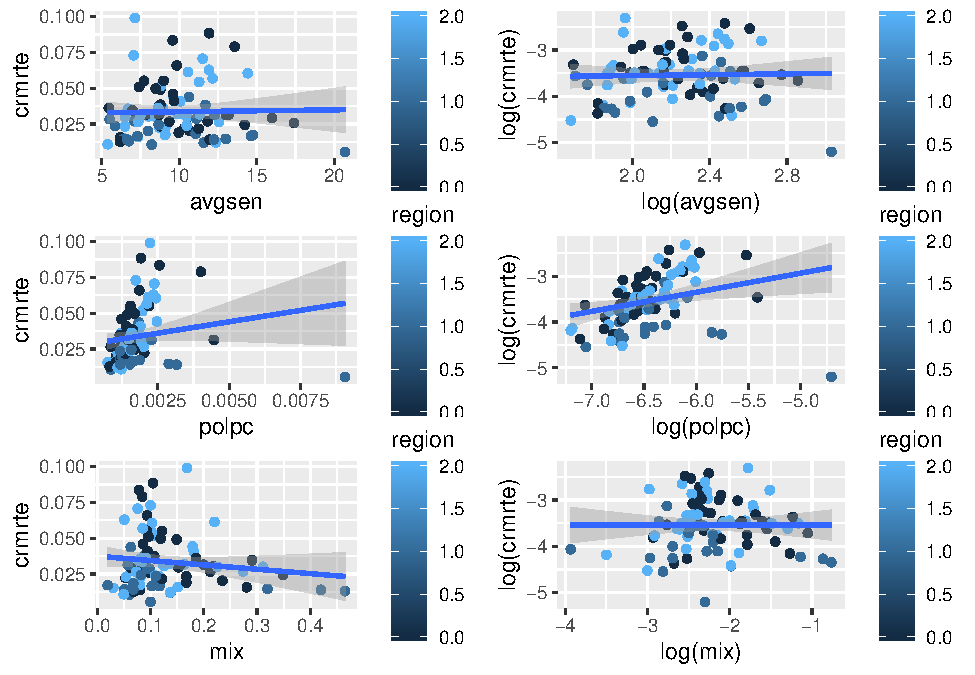
\includegraphics{Bagnard_Gaustad_Hartman_Leung_Lab_3_files/figure-latex/unnamed-chunk-49-2.pdf}

The log transformation for these variables makes the relationship more
linear. We will transform these variables to their log equivalents.

We also note that of the six variables, only prbarr, prbconv and polpc
show univariate correlation with crime. We believe these will be better
candidates for our model selection. Further, we see mix has no
correlation with crmrate and may be its own outcome variable.

\begin{Shaded}
\begin{Highlighting}[]
\NormalTok{dfCrime}\OperatorTok{$}\NormalTok{logprbarr <-}\StringTok{ }\KeywordTok{log}\NormalTok{(dfCrime}\OperatorTok{$}\NormalTok{prbarr)}
\NormalTok{dfCrime}\OperatorTok{$}\NormalTok{logprbconv <-}\StringTok{ }\KeywordTok{log}\NormalTok{(dfCrime}\OperatorTok{$}\NormalTok{prbconv)}
\NormalTok{dfCrime}\OperatorTok{$}\NormalTok{logprbpris <-}\StringTok{ }\KeywordTok{log}\NormalTok{(dfCrime}\OperatorTok{$}\NormalTok{prbpris)}
\NormalTok{dfCrime}\OperatorTok{$}\NormalTok{logavgsen <-}\StringTok{ }\KeywordTok{log}\NormalTok{(dfCrime}\OperatorTok{$}\NormalTok{avgsen)}
\NormalTok{dfCrime}\OperatorTok{$}\NormalTok{logpolpc <-}\StringTok{ }\KeywordTok{log}\NormalTok{(dfCrime}\OperatorTok{$}\NormalTok{polpc)}
\NormalTok{dfCrime}\OperatorTok{$}\NormalTok{logmix <-}\StringTok{ }\KeywordTok{log}\NormalTok{(dfCrime}\OperatorTok{$}\NormalTok{mix)}
\end{Highlighting}
\end{Shaded}

Next we take a look at the demographic variables and their log
alternatives

\begin{Shaded}
\begin{Highlighting}[]
\NormalTok{q1<-}\KeywordTok{ggplot}\NormalTok{(}\DataTypeTok{data =}\NormalTok{ dfCrime, }\KeywordTok{aes}\NormalTok{(}\DataTypeTok{x =}\NormalTok{ pctymle, }\DataTypeTok{y =}\NormalTok{ crmrte, }\DataTypeTok{color =}\NormalTok{ region)) }\OperatorTok{+}\StringTok{ }
\StringTok{      }\KeywordTok{geom_point}\NormalTok{()}\OperatorTok{+}
\StringTok{  }\KeywordTok{geom_smooth}\NormalTok{(}\DataTypeTok{method =} \StringTok{"lm"}\NormalTok{)}
\NormalTok{q1a<-}\KeywordTok{ggplot}\NormalTok{(}\DataTypeTok{data =}\NormalTok{ dfCrime, }\KeywordTok{aes}\NormalTok{(}\DataTypeTok{x =} \KeywordTok{log}\NormalTok{(pctymle), }\DataTypeTok{y =} \KeywordTok{log}\NormalTok{(crmrte), }\DataTypeTok{color =}\NormalTok{ region)) }\OperatorTok{+}\StringTok{ }
\StringTok{      }\KeywordTok{geom_point}\NormalTok{()}\OperatorTok{+}
\StringTok{  }\KeywordTok{geom_smooth}\NormalTok{(}\DataTypeTok{method =} \StringTok{"lm"}\NormalTok{)}
\NormalTok{q2<-}\KeywordTok{ggplot}\NormalTok{(}\DataTypeTok{data =}\NormalTok{ dfCrime, }\KeywordTok{aes}\NormalTok{(}\DataTypeTok{x =}\NormalTok{ pctmin80, }\DataTypeTok{y =}\NormalTok{ crmrte, }\DataTypeTok{color =}\NormalTok{ region)) }\OperatorTok{+}\StringTok{ }
\StringTok{      }\KeywordTok{geom_point}\NormalTok{()}\OperatorTok{+}
\StringTok{  }\KeywordTok{geom_smooth}\NormalTok{(}\DataTypeTok{method =} \StringTok{"lm"}\NormalTok{)}
\NormalTok{q2a<-}\KeywordTok{ggplot}\NormalTok{(}\DataTypeTok{data =}\NormalTok{ dfCrime, }\KeywordTok{aes}\NormalTok{(}\DataTypeTok{x =} \KeywordTok{log}\NormalTok{(pctmin80), }\DataTypeTok{y =} \KeywordTok{log}\NormalTok{(crmrte), }\DataTypeTok{color =}\NormalTok{ region)) }\OperatorTok{+}\StringTok{ }
\StringTok{      }\KeywordTok{geom_point}\NormalTok{()}\OperatorTok{+}
\StringTok{  }\KeywordTok{geom_smooth}\NormalTok{(}\DataTypeTok{method =} \StringTok{"lm"}\NormalTok{)}
\NormalTok{q3<-}\KeywordTok{ggplot}\NormalTok{(}\DataTypeTok{data =}\NormalTok{ dfCrime, }\KeywordTok{aes}\NormalTok{(}\DataTypeTok{x =}\NormalTok{ density, }\DataTypeTok{y =}\NormalTok{ crmrte, }\DataTypeTok{color =}\NormalTok{ region)) }\OperatorTok{+}\StringTok{ }
\StringTok{      }\KeywordTok{geom_point}\NormalTok{()}\OperatorTok{+}
\StringTok{  }\KeywordTok{geom_smooth}\NormalTok{(}\DataTypeTok{method =} \StringTok{"lm"}\NormalTok{)}
\NormalTok{q3a<-}\KeywordTok{ggplot}\NormalTok{(}\DataTypeTok{data =}\NormalTok{ dfCrime, }\KeywordTok{aes}\NormalTok{(}\DataTypeTok{x =} \KeywordTok{log}\NormalTok{(density), }\DataTypeTok{y =} \KeywordTok{log}\NormalTok{(crmrte), }\DataTypeTok{color =}\NormalTok{ region)) }\OperatorTok{+}\StringTok{ }
\StringTok{      }\KeywordTok{geom_point}\NormalTok{()}\OperatorTok{+}
\StringTok{  }\KeywordTok{geom_smooth}\NormalTok{(}\DataTypeTok{method =} \StringTok{"lm"}\NormalTok{)}


\KeywordTok{grid.arrange}\NormalTok{(q1, q1a, q2, q2a, q3, q3a, }\DataTypeTok{ncol=}\DecValTok{2}\NormalTok{)}
\end{Highlighting}
\end{Shaded}

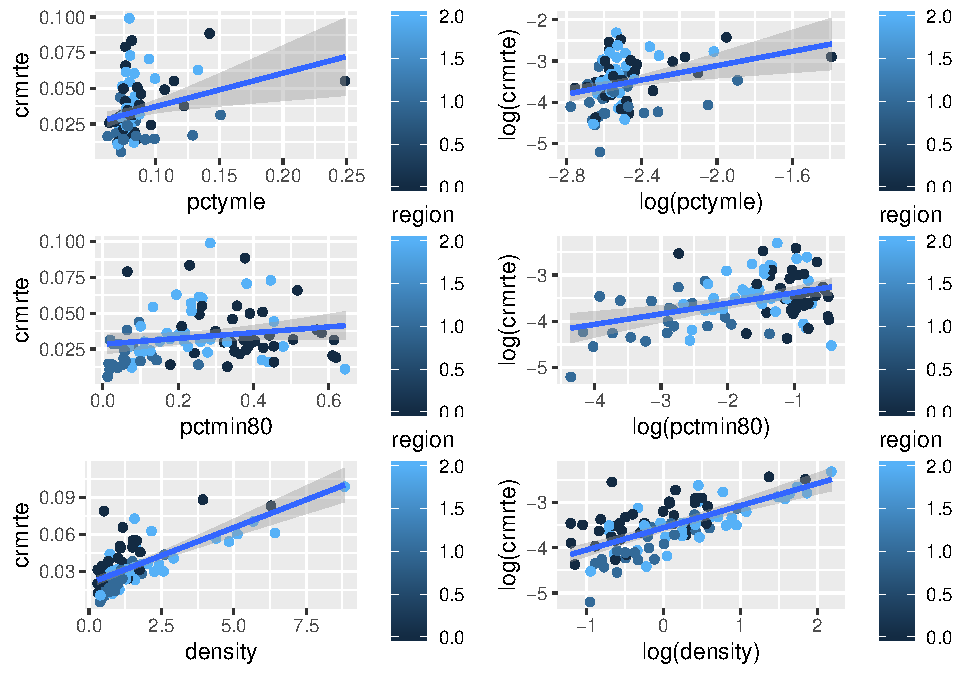
\includegraphics{Bagnard_Gaustad_Hartman_Leung_Lab_3_files/figure-latex/unnamed-chunk-51-1.pdf}

Again we see improvements after transformation. We will include
transforms of these variables as well.

\begin{Shaded}
\begin{Highlighting}[]
\NormalTok{dfCrime}\OperatorTok{$}\NormalTok{logdensity <-}\StringTok{ }\KeywordTok{log}\NormalTok{(dfCrime}\OperatorTok{$}\NormalTok{density)}
\NormalTok{dfCrime}\OperatorTok{$}\NormalTok{logpctmin80 <-}\StringTok{ }\KeywordTok{log}\NormalTok{(dfCrime}\OperatorTok{$}\NormalTok{pctmin80)}
\NormalTok{dfCrime}\OperatorTok{$}\NormalTok{logpctymle <-}\StringTok{ }\KeywordTok{log}\NormalTok{(dfCrime}\OperatorTok{$}\NormalTok{pctymle)}
\end{Highlighting}
\end{Shaded}

Finally, we'll take a look at taxpc and a histogram of the crmrte
variable itself.

\begin{Shaded}
\begin{Highlighting}[]
\NormalTok{q1<-}\KeywordTok{ggplot}\NormalTok{(}\DataTypeTok{data =}\NormalTok{ dfCrime, }\KeywordTok{aes}\NormalTok{(}\DataTypeTok{x =}\NormalTok{ taxpc, }\DataTypeTok{y =}\NormalTok{ crmrte, }\DataTypeTok{color =}\NormalTok{ region)) }\OperatorTok{+}\StringTok{ }
\StringTok{      }\KeywordTok{geom_point}\NormalTok{()}\OperatorTok{+}
\StringTok{  }\KeywordTok{geom_smooth}\NormalTok{(}\DataTypeTok{method =} \StringTok{"lm"}\NormalTok{)}
\NormalTok{q1a<-}\KeywordTok{ggplot}\NormalTok{(}\DataTypeTok{data =}\NormalTok{ dfCrime, }\KeywordTok{aes}\NormalTok{(}\DataTypeTok{x =} \KeywordTok{log}\NormalTok{(taxpc), }\DataTypeTok{y =} \KeywordTok{log}\NormalTok{(crmrte), }\DataTypeTok{color =}\NormalTok{ region)) }\OperatorTok{+}\StringTok{ }
\StringTok{      }\KeywordTok{geom_point}\NormalTok{()}\OperatorTok{+}
\StringTok{  }\KeywordTok{geom_smooth}\NormalTok{(}\DataTypeTok{method =} \StringTok{"lm"}\NormalTok{)}

\NormalTok{q2<-}\KeywordTok{ggplot}\NormalTok{(}\DataTypeTok{data =}\NormalTok{ dfCrime, }\KeywordTok{aes}\NormalTok{(}\DataTypeTok{x =}\NormalTok{ crmrte)) }\OperatorTok{+}\StringTok{ }
\StringTok{      }\KeywordTok{geom_histogram}\NormalTok{(}\DataTypeTok{bins=}\DecValTok{30}\NormalTok{)}
\NormalTok{q2a<-}\KeywordTok{ggplot}\NormalTok{(}\DataTypeTok{data =}\NormalTok{ dfCrime, }\KeywordTok{aes}\NormalTok{(}\DataTypeTok{x =} \KeywordTok{log}\NormalTok{(crmrte))) }\OperatorTok{+}\StringTok{ }
\StringTok{      }\KeywordTok{geom_histogram}\NormalTok{(}\DataTypeTok{bins=}\DecValTok{30}\NormalTok{)}

\KeywordTok{grid.arrange}\NormalTok{(q1, q1a, q2, q2a, }\DataTypeTok{ncol=}\DecValTok{2}\NormalTok{)}
\end{Highlighting}
\end{Shaded}

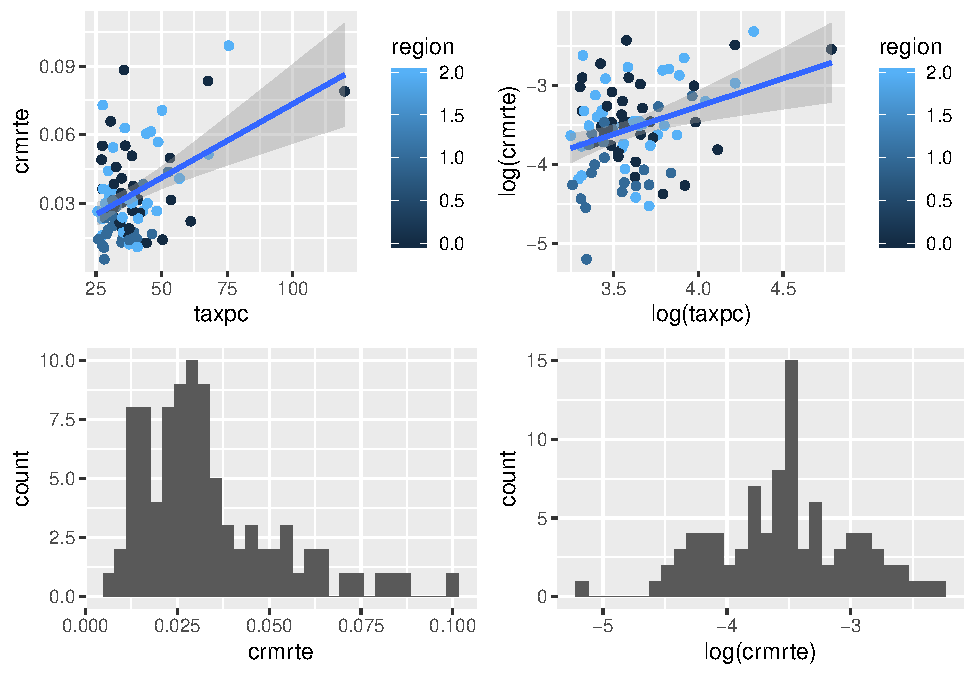
\includegraphics{Bagnard_Gaustad_Hartman_Leung_Lab_3_files/figure-latex/unnamed-chunk-53-1.pdf}

The crmrte and taxpc variables also show improvement after
transformation. We'll add those to our dataframe.

\begin{Shaded}
\begin{Highlighting}[]
\NormalTok{dfCrime}\OperatorTok{$}\NormalTok{logcrmrte =}\StringTok{ }\KeywordTok{log}\NormalTok{(dfCrime}\OperatorTok{$}\NormalTok{crmrte)}
\NormalTok{dfCrime}\OperatorTok{$}\NormalTok{logtaxpc =}\StringTok{ }\KeywordTok{log}\NormalTok{(dfCrime}\OperatorTok{$}\NormalTok{taxpc)}
\end{Highlighting}
\end{Shaded}

With our variables transformed, we now turn to discussion on
collinearity and multicollinearity in our data set. To facilitate the
discussion we'll draw reference to a network plot.

\begin{Shaded}
\begin{Highlighting}[]
\KeywordTok{options}\NormalTok{(}\DataTypeTok{repr.plot.width=}\DecValTok{8}\NormalTok{, }\DataTypeTok{repr.plot.height=}\DecValTok{8}\NormalTok{)}
\NormalTok{myData<-dfCrime}
\NormalTok{myData<-myData[, }\KeywordTok{c}\NormalTok{(}\StringTok{"logcrmrte"}\NormalTok{, }\StringTok{"west"}\NormalTok{, }\StringTok{"central"}\NormalTok{, }\StringTok{"other"}\NormalTok{, }\StringTok{"urban"}\NormalTok{, }\StringTok{"logprbarr"}\NormalTok{, }\StringTok{"logprbconv"}\NormalTok{, }\StringTok{"logprbpris"}\NormalTok{, }\StringTok{"logavgsen"}\NormalTok{, }\StringTok{"logpolpc"}\NormalTok{, }\StringTok{"logtaxpc"}\NormalTok{,}
           \StringTok{"logpctmin80"}\NormalTok{, }\StringTok{"logwcon"}\NormalTok{, }\StringTok{"logwtuc"}\NormalTok{, }\StringTok{"logwtrd"}\NormalTok{, }\StringTok{"logwfir"}\NormalTok{, }\StringTok{"logwser"}\NormalTok{, }\StringTok{"logwmfg"}\NormalTok{, }\StringTok{"logwfed"}\NormalTok{, }\StringTok{"logwsta"}\NormalTok{, }\StringTok{"logwloc"}\NormalTok{,}
           \StringTok{"logmix"}\NormalTok{, }\StringTok{"logpctymle"}\NormalTok{, }\StringTok{"logdensity"}\NormalTok{)]}
\NormalTok{plot<-myData }\OperatorTok\StringTok{ }\KeywordTok{correlate}\NormalTok{() }\OperatorTok\StringTok{ }\KeywordTok{network_plot}\NormalTok{(}\DataTypeTok{min_cor=}\NormalTok{.}\DecValTok{25}\NormalTok{)}
\end{Highlighting}
\end{Shaded}

\begin{verbatim}

Correlation method: 'pearson'
Missing treated using: 'pairwise.complete.obs'
\end{verbatim}

\begin{Shaded}
\begin{Highlighting}[]
\KeywordTok{grid.arrange}\NormalTok{(}\KeywordTok{arrangeGrob}\NormalTok{(plot, }\DataTypeTok{bottom =} \StringTok{'Correlations Among Variables'}\NormalTok{), }
             \DataTypeTok{top =} \StringTok{"Network plot for Correlation Study"}\NormalTok{, }\DataTypeTok{ncol=}\DecValTok{1}\NormalTok{)}
\end{Highlighting}
\end{Shaded}

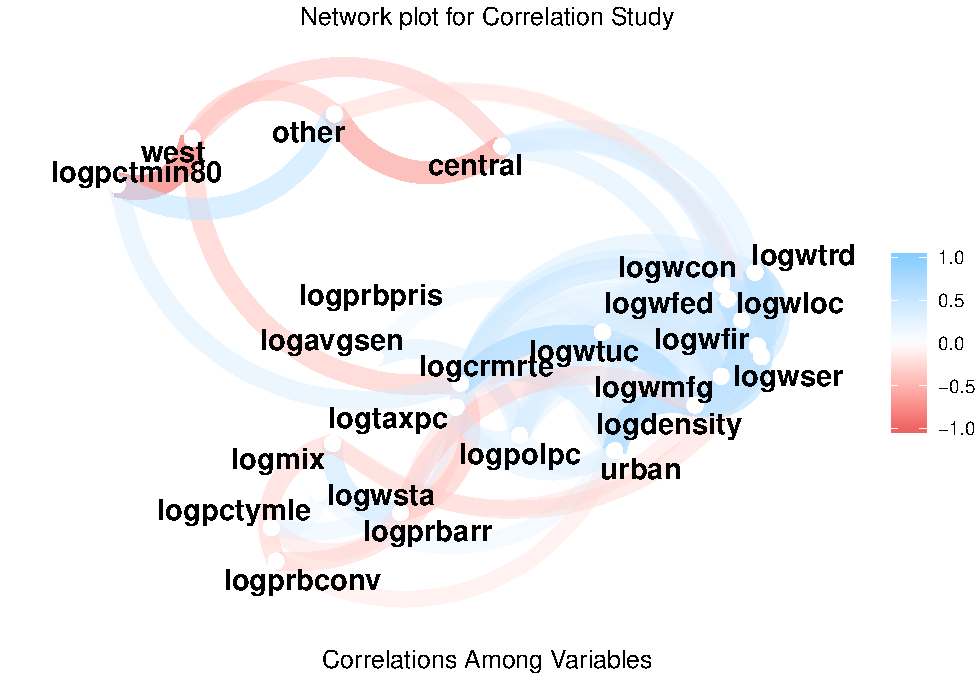
\includegraphics{Bagnard_Gaustad_Hartman_Leung_Lab_3_files/figure-latex/unnamed-chunk-55-1.pdf}
First, we note the general proximity of variables with one another.
Variables that are clustered together have stronger affinities and
degrees of collinearity. In fact, the cluster of the wage variables are
an indication of multicollinearity. Only state wages fall outside this
group. The telecome and utlity wage variable, while still near the
cluster, show a little less collinearity. If we choose to operationalize
the wage variables we must pick an appropriate strategy to minimize
their multicollinearity impact. We also see the wage variables are
positively correlated with our crime outcome variable. Density also
positively correlates with wage and the crime rate variable. Urban also
correlates with wage, but suprisingly the correlation between crime and
urban is not as high.

Next, we notice the Law enforcement and Judicial variables are clustered
and have a negative correlation with our outcome variable on crime. We
also see they tend to be negatively correlated amongst one another. For
example, probability of conviction is slightly negatively corrrelated
with the probability of arrest, and both are negatively correlated with
our outcome variable. We may wish to combine their impacts. We also see
that police per capita and tax per capita are positively correlated with
another. This makes sense as the more revenues collected the higher the
ability to pay for community services such as law enforcement and
protection. Both are also positively correlated with our outcome
variable on crime. We also notice that percent young male has a positive
correlation with crime rate. A possible explanation for this is that
more crimes are committed by younger men as a whole. We also note that
counties with higher state wages are correlated with higher percentages
of young males, and these two variables are clustered together.

The mix variable is an odd one. It is positively correlated with
probability of arrests, negatively correlated with probability of
convictions, and negatively correlated with service wages and
manufacturing wages. It also has a slight positive correlation with the
state wage and seems to be clustered with it.

Last, we turn to our region variables and notice the high negative
correlation of the minority variable with the western region. We also
notice a high positive corrlation of minorities with the `other'
(eastern) region. This variable also correlates positively with crime
rate, although the two are not clustered. We especially note that west
is negatively correlated with crime rate. There appears to be a lessor
propensity for crime in this region. We will examine this phenomenom
further. Also, for a futher examination of correlation plots for each of
the regions please see the network diagrams in the appendix.

\hypertarget{additional-variables-to-operationalize}{%
\subsection{Additional Variables to
Operationalize}\label{additional-variables-to-operationalize}}

As a final point of discussion we will identify variables we wish to
operationalize for use in our models. We will include a variable that
expresses the economic condition of the county and a variable that
expresses criminal justice effectiveness.

The first variable on the economic condition will include the sum of all
average weekly wages from the 1980 census information. Since we do not
know how many were employed at that wage we use this summary the best
available proxy. Summing the wages into one variable will also remove
their multicollinearity effects.

\begin{Shaded}
\begin{Highlighting}[]
\NormalTok{dfCrime}\OperatorTok{$}\NormalTok{allWages<-dfCrime}\OperatorTok{$}\NormalTok{wcon }\OperatorTok{+}\StringTok{ }\NormalTok{dfCrime}\OperatorTok{$}\NormalTok{wtuc }\OperatorTok{+}\StringTok{ }\NormalTok{dfCrime}\OperatorTok{$}\NormalTok{wtrd }\OperatorTok{+}\StringTok{ }\NormalTok{dfCrime}\OperatorTok{$}\NormalTok{wfir }\OperatorTok{+}
\StringTok{    }\NormalTok{dfCrime}\OperatorTok{$}\NormalTok{wser }\OperatorTok{+}\StringTok{ }\NormalTok{dfCrime}\OperatorTok{$}\NormalTok{wmfg }\OperatorTok{+}\StringTok{ }\NormalTok{dfCrime}\OperatorTok{$}\NormalTok{wfed }\OperatorTok{+}\StringTok{ }\NormalTok{dfCrime}\OperatorTok{$}\NormalTok{wsta }\OperatorTok{+}\StringTok{ }\NormalTok{dfCrime}\OperatorTok{$}\NormalTok{wloc}
\end{Highlighting}
\end{Shaded}

As a second variable, we are interested in understanding the
effectiveness of the criminal justice system as a crime deterrent. Our
proxy will be the number of convictions per incident.

This is operationalized by taking the probability of arrests, pbrarr
(which is defined as arrests per incident) and multiplying by the
probability of convictions, pbrconv (which is defined as convictions per
arrest). The new variable is defined below.

\begin{Shaded}
\begin{Highlighting}[]
\NormalTok{dfCrime}\OperatorTok{$}\NormalTok{crimJustEff<-dfCrime}\OperatorTok{$}\NormalTok{prbarr }\OperatorTok{*}\StringTok{ }\NormalTok{dfCrime}\OperatorTok{$}\NormalTok{prbconv}
\end{Highlighting}
\end{Shaded}

We will also create a logarithmic transformation of this variable based
on our histogram analysis from before.

\begin{Shaded}
\begin{Highlighting}[]
\NormalTok{dfCrime}\OperatorTok{$}\NormalTok{logcrimJustEff<-}\KeywordTok{log}\NormalTok{(dfCrime}\OperatorTok{$}\NormalTok{crimJustEff)}
\end{Highlighting}
\end{Shaded}

\hypertarget{summary-and-results}{%
\subsection{Summary and Results}\label{summary-and-results}}

Our outcome variable is the \emph{crime rate} (``crmrte''), which is
defined as the crimes committed per person in a specific county during
1987. The crime rate of the 90 counties in our sample dataset range
between 0.0055 - 0.0990, with a mean of 0.0335.

From the boxplot below, most of the counties have a crime rate between
0.0055 and 0.0700, with 5 outliers having a crime rate \textgreater{}
0.0700.

\begin{Shaded}
\begin{Highlighting}[]
\KeywordTok{options}\NormalTok{(}\DataTypeTok{repr.plot.width=}\DecValTok{3}\NormalTok{, }\DataTypeTok{repr.plot.height=}\DecValTok{4}\NormalTok{)}
\KeywordTok{ggplot}\NormalTok{(}\DataTypeTok{data =}\NormalTok{ dfCrime, }\KeywordTok{aes}\NormalTok{(}\DataTypeTok{y =}\NormalTok{ crmrte)) }\OperatorTok{+}\StringTok{ }
\StringTok{      }\KeywordTok{geom_boxplot}\NormalTok{()}
\end{Highlighting}
\end{Shaded}

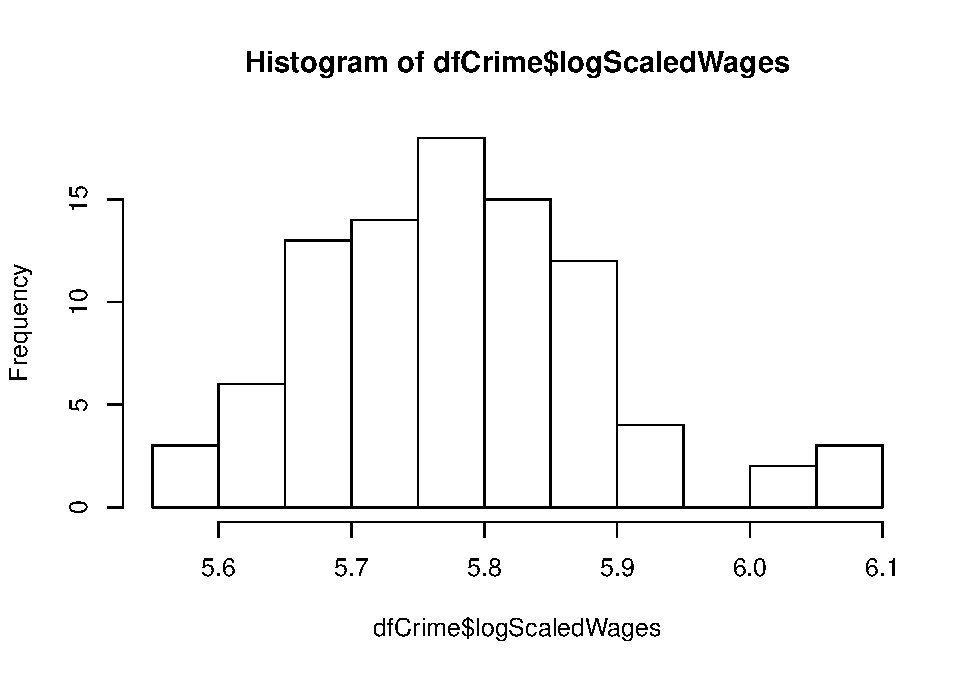
\includegraphics{Bagnard_Gaustad_Hartman_Leung_Lab_3_files/figure-latex/unnamed-chunk-59-1.pdf}

While mix (the type of crime committed) is also potentially an outcome
variable, our research focuses on providing policy recommendations to
reduce crime in general and not a specific type of crime. Mix is also
not a linear outcome and hence difficult to measure.

We propose 3 multiple linear regression models

\begin{itemize}
\item
  First Model: Has only the explanatory variables of key interest and no
  other covariates.
\item
  Second Model: Includes the explanatory variables and covariates that
  increase the accuracy of our results without substantial bias.
\item
  Third Model: An expansion of the second model with most covariates,
  designed to demonstrate the robustness of our results to model
  specification.
\end{itemize}

As we proceed with each model, we verify the CLM assumptions of OLS are
addressed below:

\begin{itemize}
\item
  \textbf{MLR1} Linear in parameters: The models have had its data
  transformed as described above to allow a linear fit of the model.
\item
  \textbf{MLR2} Random Sampling: The data is collected from a data set
  with rolled up data for each county. It is not randomly sampled by
  area or population.
\item
  \textbf{MLR3} to be discussed on a model by model basis.
\item
  \textbf{MLR4} to be discussed on a model by model basis.
\item
  \textbf{MLR5'} to be discussed on a model by model basis.
\item
  \textbf{MLR6'} to be discussed on a model by model basis.
\end{itemize}

By satisfying these assumptions, we can expect our coefficients will be
approaching the true parameter values in probability.

\hypertarget{model-analysis}{%
\section{Model Analysis}\label{model-analysis}}

\hypertarget{model-1}{%
\subsection{Model 1}\label{model-1}}

\hypertarget{introduction-1}{%
\subsubsection{Introduction}\label{introduction-1}}

Our base hypothesis is that crime can be fundamentally explained by two
factors: the effectiveness of the criminal justice system and the
economic conditions.

Criminal Justice Effectiveness is self defined : To be able to track
crimes, they must be reported to police, who can then make arrests and
the legal system provides judgement (convictions/sentencing).\\
Criminal justice also has a relationship to crime as a deterrent, as the
probability of getting caught, convicted, sentenced could potentially
deter crime.

We operationalize criminal justice effectiveness as (probability of
Convictions * Crimes committed). We define this as: prbconv * prbarr =
conv/arrest * arrest/crime = convictions/crime. Without more granular
data, this provides a single parsimonious metric that helps understand
how well the law enforcement and criminal justice system works.

We theorize that the second major cause of crime are bad economic
conditions. When there are worse economic conditions, crime can be
increased due to:

\begin{itemize}
\tightlist
\item
  Lack of means: People forced into crimes because they need to make
  ends meet
\item
  Lack of occupation: People commit crimes because they are not busy at
  work
\item
  Lack of opportunity: High discount rate for future due to no long-term
  opportunity, incentive to take the risk and commit crimes hoping for
  big payoff.
\end{itemize}

We operationalize economic conditions by looking at wages. For this
model, we define this as the unweighted average weekly pay from each
sector provided in the data set. We think this is best proxy from our
data because it answers all of the above (higher wages leads to better
means and better opportunities). From our EDA we also confirm that in
general these sums are not skewed by having 1 really high paying sector
in each county as we see a strong relationship between avg quartile
across all job types and total sum. This can be seen in the chart below.

\hypertarget{model-1-eda}{%
\subsubsection{Model 1 EDA}\label{model-1-eda}}

\textbf{Data Transformations}

\begin{Shaded}
\begin{Highlighting}[]
\KeywordTok{options}\NormalTok{(}\DataTypeTok{repr.plot.width=}\DecValTok{4}\NormalTok{, }\DataTypeTok{repr.plot.height=}\DecValTok{4}\NormalTok{)}
\KeywordTok{hist}\NormalTok{((dfCrime}\OperatorTok{$}\NormalTok{prbconv))}
\end{Highlighting}
\end{Shaded}

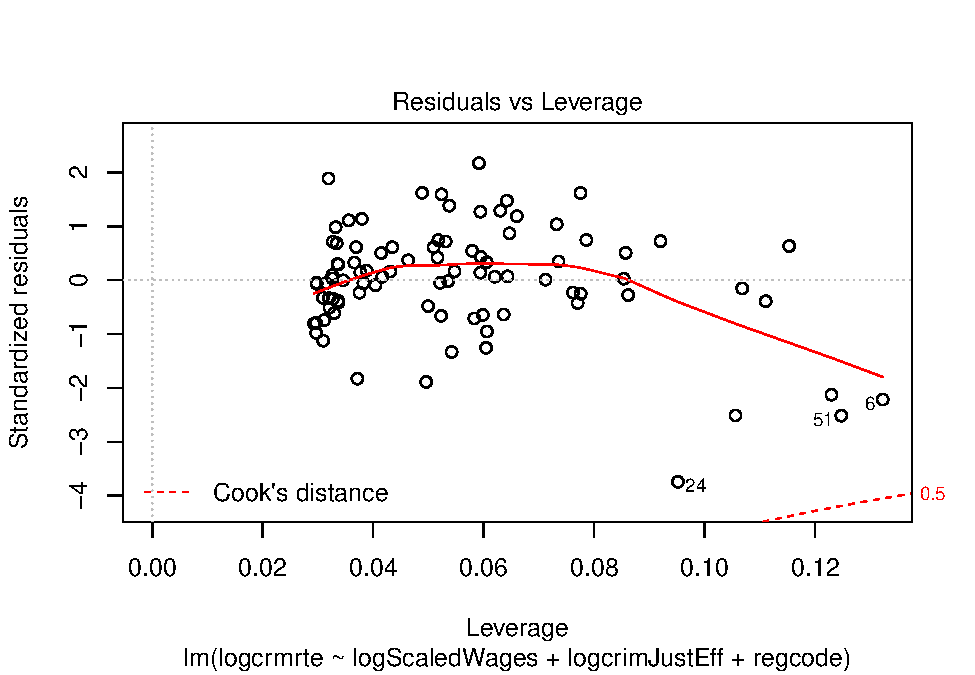
\includegraphics{Bagnard_Gaustad_Hartman_Leung_Lab_3_files/figure-latex/unnamed-chunk-60-1.pdf}

\begin{Shaded}
\begin{Highlighting}[]
\KeywordTok{hist}\NormalTok{((dfCrime}\OperatorTok{$}\NormalTok{prbarr))}
\end{Highlighting}
\end{Shaded}

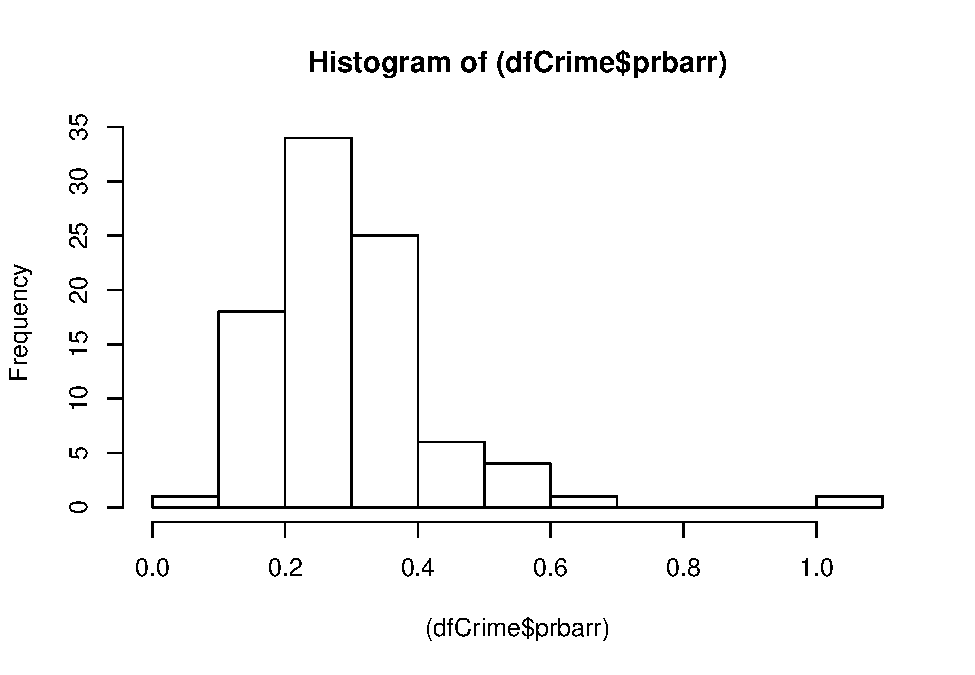
\includegraphics{Bagnard_Gaustad_Hartman_Leung_Lab_3_files/figure-latex/unnamed-chunk-60-2.pdf}

The distribution of both probability of conviction and probability of
arrest are peculiar and non-normal. It could be argued that both of
these variables should be bound between 0 and 1. However,
``probability'' of conviction is proxied by a ratio of convictions to
arrests. It is in fact common that defendents are charged with multiple
crimes and convicted, but were only arrested once.

For ``probability'' of arrest, it could be possible there are multiple
arrests for a single offense. However, the single data point that is
greater than one, is \textgreater{}3 standard deviations away from the
distribution. Since this value falls so far out of distribution it will
have high leverage on our model and will be preemptively imputed as the
data supplied is likely in error and is not representative of the bulk
of North Carolina counties.

For parsimony, we can simply the probability of arrest and probability
of conviction by multiplying to effectively get the ratio of convictions
to offenses. The normality of this factor can be improved by taking a
log transform. QQ plots help to visualize how normality improves for the
inner quartiles.

\begin{Shaded}
\begin{Highlighting}[]
\CommentTok{# how many standard deviations away the outlier lies}
\NormalTok{(dfCrime[}\DecValTok{51}\NormalTok{,]}\OperatorTok{$}\NormalTok{prbarr }\OperatorTok{-}\StringTok{ }\KeywordTok{mean}\NormalTok{(dfCrime}\OperatorTok{$}\NormalTok{prbarr))}\OperatorTok{/}\KeywordTok{sd}\NormalTok{(dfCrime}\OperatorTok{$}\NormalTok{prbarr) }
\end{Highlighting}
\end{Shaded}

\begin{verbatim}
[1] 5.779438
\end{verbatim}

\begin{Shaded}
\begin{Highlighting}[]
\CommentTok{#hist(log(dfCrime$crimJustEff))}
\KeywordTok{ggplot}\NormalTok{(}\DataTypeTok{data=}\NormalTok{dfCrime, }\KeywordTok{aes}\NormalTok{(}\DataTypeTok{sample=}\NormalTok{ crimJustEff)) }\OperatorTok{+}\StringTok{ }\KeywordTok{stat_qq}\NormalTok{() }\OperatorTok{+}\StringTok{ }\KeywordTok{stat_qq_line}\NormalTok{() }\OperatorTok{+}\StringTok{ }
\StringTok{  }\KeywordTok{ggtitle}\NormalTok{(}\StringTok{"QQ Plot of Crim Just Eff"}\NormalTok{)}
\end{Highlighting}
\end{Shaded}

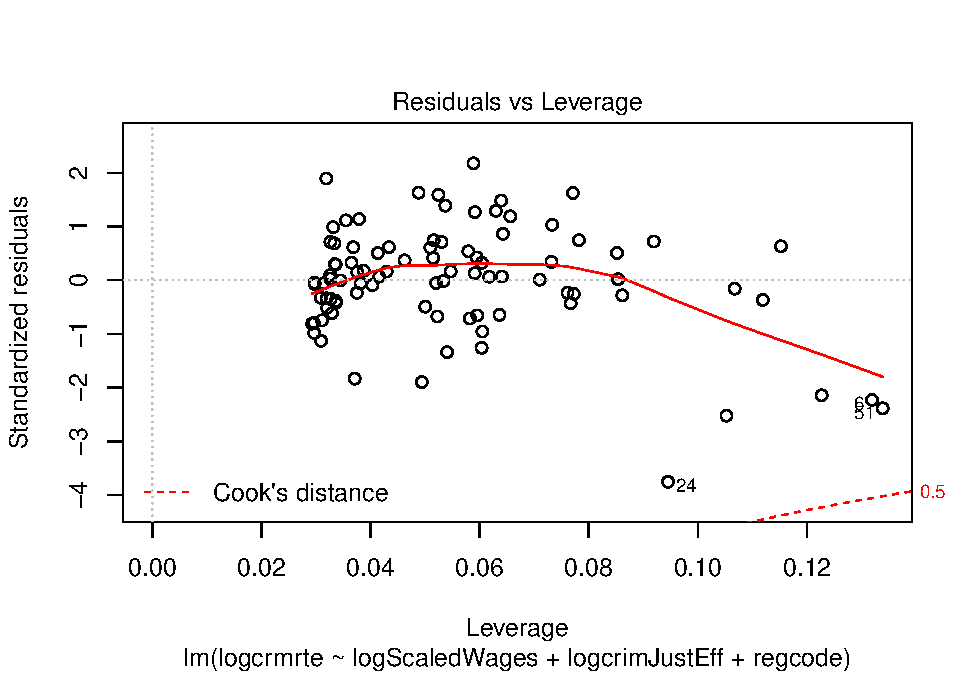
\includegraphics{Bagnard_Gaustad_Hartman_Leung_Lab_3_files/figure-latex/unnamed-chunk-61-1.pdf}

\begin{Shaded}
\begin{Highlighting}[]
\NormalTok{dfCrime[dfCrime}\OperatorTok{$}\NormalTok{crimJustEff }\OperatorTok{>}\StringTok{ }\DecValTok{1}\NormalTok{,] }\CommentTok{# find outlier}
\end{Highlighting}
\end{Shaded}

\begin{verbatim}
   county year    crmrte  prbarr prbconv prbpris avgsen      polpc
51    115   87 0.0055332 1.09091     1.5     0.5   20.7 0.00905433
     density   taxpc west central urban  pctmin80     wcon     wtuc
51 0.3858093 28.1931    1       0     0 0.0128365 204.2206 503.2351
       wtrd     wfir     wser   wmfg  wfed   wsta   wloc mix    pctymle
51 217.4908 342.4658 245.2061 448.42 442.2 340.39 386.12 0.1 0.07253495
   region regcode other nonurban         metro  logwcon  logwtuc  logwtrd
51      1    West     0        1 Outside Metro 5.319201 6.221057 5.382157
    logwfir  logwser logwmfg  logwfed  logwsta  logwloc  logprbarr
51 5.836172 5.502099 6.10573 6.091762 5.830092 5.956148 0.08701217
   logprbconv logprbpris logavgsen  logpolpc    logmix logdensity
51  0.4054651 -0.6931472  3.030134 -4.704512 -2.302585 -0.9524121
   logpctmin80 logpctymle logcrmrte logtaxpc allWages crimJustEff
51   -4.355463  -2.623687 -5.196989 3.339077 3129.748    1.636365
   logcrimJustEff
51      0.4924773
\end{verbatim}

We will use the imputation method to replace the large prbarr value and
remove the outlier effect, while also retaining the rest of the
variables in the county.

---delete---- We also see that polpc is .009. We noticed this outlier
during our EDA analysis. Based on the records describing the US
population on police officers per capita, the highest police per capita
on record is .007 in Atlantic City, NJ.
\url{https://www.governing.com/gov-data/safety-justice/police-officers-per-capita-rates-employment-for-city-departments.html}
This datapoint is also in error and we will impute it's replacement.
---/delete---

\begin{Shaded}
\begin{Highlighting}[]
\NormalTok{dfCrime}\OperatorTok{$}\NormalTok{prbarr[}\KeywordTok{which}\NormalTok{(dfCrime}\OperatorTok{$}\NormalTok{county}\OperatorTok{==}\DecValTok{115}\NormalTok{)]<-}\OtherTok{NA} \CommentTok{# set the value to NA so it will be imputed}
\CommentTok{#dfCrime$prbconv[which(dfCrime$county==115)]<-NA # set the value to NA so it will be imputed}
\CommentTok{#dfCrime$polpc[which(dfCrime$county==115)]<-NA # set the value to NA so it will be imputed delete}
\end{Highlighting}
\end{Shaded}

\begin{Shaded}
\begin{Highlighting}[]
\NormalTok{impute_arg <-}\StringTok{ }\KeywordTok{aregImpute}\NormalTok{(}\OperatorTok{~}\StringTok{ }\NormalTok{crmrte }\OperatorTok{+}\StringTok{  }\NormalTok{urban }\OperatorTok{+}\StringTok{ }\NormalTok{central }\OperatorTok{+}\StringTok{ }\NormalTok{west }\OperatorTok{+}\StringTok{ }\NormalTok{other }\OperatorTok{+}
\StringTok{                         }\NormalTok{prbarr }\OperatorTok{+}\StringTok{ }\NormalTok{prbconv }\OperatorTok{+}\StringTok{ }\NormalTok{prbpris }\OperatorTok{+}\StringTok{ }\NormalTok{avgsen }\OperatorTok{+}\StringTok{ }\NormalTok{polpc }\OperatorTok{+}\StringTok{ }
\StringTok{                         }\NormalTok{density }\OperatorTok{+}\StringTok{ }\NormalTok{taxpc }\OperatorTok{+}\StringTok{ }\NormalTok{pctmin80 }\OperatorTok{+}\StringTok{ }\NormalTok{wcon }\OperatorTok{+}\StringTok{ }\NormalTok{wtuc }\OperatorTok{+}
\StringTok{                         }\NormalTok{wtrd }\OperatorTok{+}\StringTok{ }\NormalTok{wfir }\OperatorTok{+}\StringTok{ }\NormalTok{wser }\OperatorTok{+}\StringTok{ }\NormalTok{wmfg }\OperatorTok{+}\StringTok{ }\NormalTok{wfed }\OperatorTok{+}\StringTok{ }\NormalTok{wsta }\OperatorTok{+}\StringTok{ }\NormalTok{wloc }\OperatorTok{+}
\StringTok{                         }\NormalTok{mix }\OperatorTok{+}\StringTok{ }\NormalTok{pctymle, }\DataTypeTok{data =}\NormalTok{ dfCrime, }\DataTypeTok{match=}\StringTok{"weighted"}\NormalTok{,}
                         \DataTypeTok{nk=}\DecValTok{3}\NormalTok{, }\DataTypeTok{B=}\DecValTok{10}\NormalTok{, }\DataTypeTok{n.impute =} \DecValTok{100}\NormalTok{)}
\end{Highlighting}
\end{Shaded}

\begin{Shaded}
\begin{Highlighting}[]
\KeywordTok{paste}\NormalTok{(}\StringTok{"R-squares for Predicting Non-Missing Values for Each Variable"}\NormalTok{)}
\end{Highlighting}
\end{Shaded}

\begin{verbatim}
[1] "R-squares for Predicting Non-Missing Values for Each Variable"
\end{verbatim}

\begin{Shaded}
\begin{Highlighting}[]
\NormalTok{impute_arg}\OperatorTok{$}\NormalTok{rsq}
\end{Highlighting}
\end{Shaded}

\begin{verbatim}
   prbarr 
0.9196967 
\end{verbatim}

\begin{Shaded}
\begin{Highlighting}[]
\KeywordTok{paste}\NormalTok{(}\StringTok{"Distribution of Values for Each Imputation"}\NormalTok{)}
\end{Highlighting}
\end{Shaded}

\begin{verbatim}
[1] "Distribution of Values for Each Imputation"
\end{verbatim}

\begin{Shaded}
\begin{Highlighting}[]
\KeywordTok{table}\NormalTok{(impute_arg}\OperatorTok{$}\NormalTok{imputed}\OperatorTok{$}\NormalTok{prbarr)}
\end{Highlighting}
\end{Shaded}

\begin{verbatim}

0.092770003 0.132028997 0.149936005 0.161381006 0.182589993 0.221542001 
          1           3           1           1           1           1 
0.238636002 0.243119001 0.251599014  0.26602599 0.266054988 0.266959995 
          1           1           1           1           2           1 
0.269042999 0.271966994 0.283504993 0.289121002 0.298269987 0.310986996 
          2           1           2           1          56           1 
0.338901997 0.350347996  0.35473299 0.362269998 0.392111003 0.444444001 
          1           1           1           2           1           1 
0.456393987 0.482425004 0.487430006 0.518218994 0.522696018 0.524663985 
          1           1           1           1           3           2 
0.530435026 0.689023972 
          2           4 
\end{verbatim}

\begin{Shaded}
\begin{Highlighting}[]
\KeywordTok{paste}\NormalTok{(}\StringTok{"Distribution of Values for Each Imputation"}\NormalTok{)}
\end{Highlighting}
\end{Shaded}

\begin{verbatim}
[1] "Distribution of Values for Each Imputation"
\end{verbatim}

\begin{Shaded}
\begin{Highlighting}[]
\KeywordTok{table}\NormalTok{(impute_arg}\OperatorTok{$}\NormalTok{imputed}\OperatorTok{$}\NormalTok{prbconv)}
\end{Highlighting}
\end{Shaded}

\begin{verbatim}
< table of extent 0 >
\end{verbatim}

\begin{Shaded}
\begin{Highlighting}[]
\KeywordTok{paste}\NormalTok{(}\StringTok{"Distribution of Values for Each Imputation"}\NormalTok{)}
\end{Highlighting}
\end{Shaded}

\begin{verbatim}
[1] "Distribution of Values for Each Imputation"
\end{verbatim}

\begin{Shaded}
\begin{Highlighting}[]
\KeywordTok{table}\NormalTok{(impute_arg}\OperatorTok{$}\NormalTok{imputed}\OperatorTok{$}\NormalTok{polpc)}
\end{Highlighting}
\end{Shaded}

\begin{verbatim}
< table of extent 0 >
\end{verbatim}

We will reassign the value in our dataset to the mean from these trials.

\begin{Shaded}
\begin{Highlighting}[]
\NormalTok{dfCrime}\OperatorTok{$}\NormalTok{prbarr[}\KeywordTok{which}\NormalTok{(dfCrime}\OperatorTok{$}\NormalTok{county}\OperatorTok{==}\DecValTok{115}\NormalTok{)]<-}\KeywordTok{mean}\NormalTok{(impute_arg}\OperatorTok{$}\NormalTok{imputed}\OperatorTok{$}\NormalTok{prbarr)}
\NormalTok{dfCrime}\OperatorTok{$}\NormalTok{prbarr[}\KeywordTok{which}\NormalTok{(dfCrime}\OperatorTok{$}\NormalTok{county}\OperatorTok{==}\DecValTok{115}\NormalTok{)]}
\end{Highlighting}
\end{Shaded}

\begin{verbatim}
[1] 0.3266697
\end{verbatim}

\begin{Shaded}
\begin{Highlighting}[]
\NormalTok{dfCrime}\OperatorTok{$}\NormalTok{prbconv[}\KeywordTok{which}\NormalTok{(dfCrime}\OperatorTok{$}\NormalTok{county}\OperatorTok{==}\DecValTok{115}\NormalTok{)]<-}\KeywordTok{mean}\NormalTok{(impute_arg}\OperatorTok{$}\NormalTok{imputed}\OperatorTok{$}\NormalTok{prbconv)}
\NormalTok{dfCrime}\OperatorTok{$}\NormalTok{prbconv[}\KeywordTok{which}\NormalTok{(dfCrime}\OperatorTok{$}\NormalTok{county}\OperatorTok{==}\DecValTok{115}\NormalTok{)]}
\end{Highlighting}
\end{Shaded}

\begin{verbatim}
[1] NA
\end{verbatim}

\begin{Shaded}
\begin{Highlighting}[]
\NormalTok{dfCrime}\OperatorTok{$}\NormalTok{polpc[}\KeywordTok{which}\NormalTok{(dfCrime}\OperatorTok{$}\NormalTok{county}\OperatorTok{==}\DecValTok{115}\NormalTok{)]<-}\KeywordTok{mean}\NormalTok{(impute_arg}\OperatorTok{$}\NormalTok{imputed}\OperatorTok{$}\NormalTok{polpc)}
\NormalTok{dfCrime}\OperatorTok{$}\NormalTok{polpc[}\KeywordTok{which}\NormalTok{(dfCrime}\OperatorTok{$}\NormalTok{county}\OperatorTok{==}\DecValTok{115}\NormalTok{)]}
\end{Highlighting}
\end{Shaded}

\begin{verbatim}
[1] NA
\end{verbatim}

\begin{Shaded}
\begin{Highlighting}[]
\NormalTok{dfCrime}\OperatorTok{$}\NormalTok{logprbarr[}\KeywordTok{which}\NormalTok{(dfCrime}\OperatorTok{$}\NormalTok{county}\OperatorTok{==}\DecValTok{115}\NormalTok{)]<-}\KeywordTok{log}\NormalTok{(dfCrime}\OperatorTok{$}\NormalTok{prbarr[}\KeywordTok{which}\NormalTok{(dfCrime}\OperatorTok{$}\NormalTok{county}\OperatorTok{==}\DecValTok{115}\NormalTok{)])}
\NormalTok{dfCrime}\OperatorTok{$}\NormalTok{logprbarr[}\KeywordTok{which}\NormalTok{(dfCrime}\OperatorTok{$}\NormalTok{county}\OperatorTok{==}\DecValTok{115}\NormalTok{)]}
\end{Highlighting}
\end{Shaded}

\begin{verbatim}
[1] -1.118806
\end{verbatim}

\begin{Shaded}
\begin{Highlighting}[]
\NormalTok{dfCrime}\OperatorTok{$}\NormalTok{logprbconv[}\KeywordTok{which}\NormalTok{(dfCrime}\OperatorTok{$}\NormalTok{county}\OperatorTok{==}\DecValTok{115}\NormalTok{)]<-}\KeywordTok{log}\NormalTok{(dfCrime}\OperatorTok{$}\NormalTok{prbconv[}\KeywordTok{which}\NormalTok{(dfCrime}\OperatorTok{$}\NormalTok{county}\OperatorTok{==}\DecValTok{115}\NormalTok{)])}
\NormalTok{dfCrime}\OperatorTok{$}\NormalTok{logprbconv[}\KeywordTok{which}\NormalTok{(dfCrime}\OperatorTok{$}\NormalTok{county}\OperatorTok{==}\DecValTok{115}\NormalTok{)]}
\end{Highlighting}
\end{Shaded}

\begin{verbatim}
[1] NA
\end{verbatim}

\begin{Shaded}
\begin{Highlighting}[]
\NormalTok{dfCrime}\OperatorTok{$}\NormalTok{logpolpc[}\KeywordTok{which}\NormalTok{(dfCrime}\OperatorTok{$}\NormalTok{county}\OperatorTok{==}\DecValTok{115}\NormalTok{)]<-}\KeywordTok{log}\NormalTok{(dfCrime}\OperatorTok{$}\NormalTok{polpc[}\KeywordTok{which}\NormalTok{(dfCrime}\OperatorTok{$}\NormalTok{county}\OperatorTok{==}\DecValTok{115}\NormalTok{)])}
\NormalTok{dfCrime}\OperatorTok{$}\NormalTok{logpolpc[}\KeywordTok{which}\NormalTok{(dfCrime}\OperatorTok{$}\NormalTok{county}\OperatorTok{==}\DecValTok{115}\NormalTok{)]}
\end{Highlighting}
\end{Shaded}

\begin{verbatim}
[1] NA
\end{verbatim}

\begin{Shaded}
\begin{Highlighting}[]
\NormalTok{dfCrime}\OperatorTok{$}\NormalTok{crimJustEff<-dfCrime}\OperatorTok{$}\NormalTok{prbarr }\OperatorTok{*}\StringTok{ }\NormalTok{dfCrime}\OperatorTok{$}\NormalTok{prbconv}
\NormalTok{dfCrime}\OperatorTok{$}\NormalTok{logcrimJustEff<-}\KeywordTok{log}\NormalTok{(dfCrime}\OperatorTok{$}\NormalTok{crimJustEff)}
\end{Highlighting}
\end{Shaded}

\begin{Shaded}
\begin{Highlighting}[]
\KeywordTok{ggplot}\NormalTok{(}\DataTypeTok{data=}\NormalTok{dfCrime, }\KeywordTok{aes}\NormalTok{(}\DataTypeTok{sample=}\NormalTok{ logcrimJustEff)) }\OperatorTok{+}\StringTok{ }\KeywordTok{stat_qq}\NormalTok{() }\OperatorTok{+}\StringTok{ }\KeywordTok{stat_qq_line}\NormalTok{() }\OperatorTok{+}\StringTok{ }
\KeywordTok{ggtitle}\NormalTok{(}\StringTok{"QQ Plot of log transformed Crim Just Eff"}\NormalTok{)}
\end{Highlighting}
\end{Shaded}

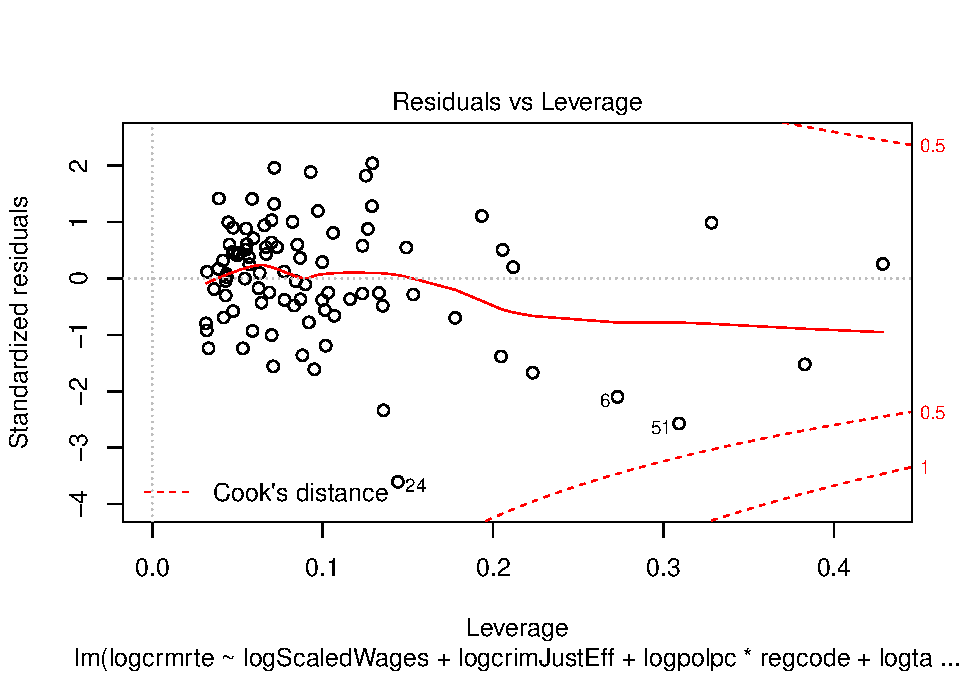
\includegraphics{Bagnard_Gaustad_Hartman_Leung_Lab_3_files/figure-latex/unnamed-chunk-72-1.pdf}

\begin{Shaded}
\begin{Highlighting}[]
\CommentTok{## Can show histogram/qqplot side by side in RMD. }
\end{Highlighting}
\end{Shaded}

For unweighted average of the wages for each sector, we can see issues.

\begin{Shaded}
\begin{Highlighting}[]
\CommentTok{# # Quantiles for all jobs}
\NormalTok{dfWage<-}\KeywordTok{mutate}\NormalTok{(dfCrime,}\DataTypeTok{qCon=}\KeywordTok{ntile}\NormalTok{(dfCrime}\OperatorTok{$}\NormalTok{wcon,}\DecValTok{4}\NormalTok{))}
\NormalTok{dfWage<-}\KeywordTok{mutate}\NormalTok{(dfWage,}\DataTypeTok{qTuc=}\KeywordTok{ntile}\NormalTok{(dfCrime}\OperatorTok{$}\NormalTok{wtuc,}\DecValTok{4}\NormalTok{))}
\NormalTok{dfWage<-}\KeywordTok{mutate}\NormalTok{(dfWage,}\DataTypeTok{qTrd=}\KeywordTok{ntile}\NormalTok{(dfCrime}\OperatorTok{$}\NormalTok{wtrd,}\DecValTok{4}\NormalTok{))}
\NormalTok{dfWage<-}\KeywordTok{mutate}\NormalTok{(dfWage,}\DataTypeTok{qFir=}\KeywordTok{ntile}\NormalTok{(dfCrime}\OperatorTok{$}\NormalTok{wfir,}\DecValTok{4}\NormalTok{))}
\NormalTok{dfWage<-}\KeywordTok{mutate}\NormalTok{(dfWage,}\DataTypeTok{qSer=}\KeywordTok{ntile}\NormalTok{(dfCrime}\OperatorTok{$}\NormalTok{wser,}\DecValTok{4}\NormalTok{))}
\NormalTok{dfWage<-}\KeywordTok{mutate}\NormalTok{(dfWage,}\DataTypeTok{qMfg=}\KeywordTok{ntile}\NormalTok{(dfCrime}\OperatorTok{$}\NormalTok{wmfg,}\DecValTok{4}\NormalTok{))}
\NormalTok{dfWage<-}\KeywordTok{mutate}\NormalTok{(dfWage,}\DataTypeTok{qFed=}\KeywordTok{ntile}\NormalTok{(dfCrime}\OperatorTok{$}\NormalTok{wfed,}\DecValTok{4}\NormalTok{))}
\NormalTok{dfWage<-}\KeywordTok{mutate}\NormalTok{(dfWage,}\DataTypeTok{qSta=}\KeywordTok{ntile}\NormalTok{(dfCrime}\OperatorTok{$}\NormalTok{wsta,}\DecValTok{4}\NormalTok{))}
\NormalTok{dfWage<-}\KeywordTok{mutate}\NormalTok{(dfWage,}\DataTypeTok{qLoc=}\KeywordTok{ntile}\NormalTok{(dfCrime}\OperatorTok{$}\NormalTok{wloc,}\DecValTok{4}\NormalTok{))}
\CommentTok{## Average quantile}
\NormalTok{dfWage}\OperatorTok{$}\NormalTok{qAvg=}\StringTok{ }\NormalTok{(dfWage}\OperatorTok{$}\NormalTok{qCon}\OperatorTok{+}\NormalTok{dfWage}\OperatorTok{$}\NormalTok{qTuc}\OperatorTok{+}\NormalTok{dfWage}\OperatorTok{$}\NormalTok{qTrd}\OperatorTok{+}\NormalTok{dfWage}\OperatorTok{$}\NormalTok{qFir}\OperatorTok{+}\NormalTok{dfWage}\OperatorTok{$}\NormalTok{qSer}\OperatorTok{+}\NormalTok{dfWage}\OperatorTok{$}\NormalTok{qMfg}\OperatorTok{+}
\StringTok{                }\NormalTok{dfWage}\OperatorTok{$}\NormalTok{qFed}\OperatorTok{+}\NormalTok{dfWage}\OperatorTok{$}\NormalTok{qSta}\OperatorTok{+}\NormalTok{dfWage}\OperatorTok{$}\NormalTok{qLoc)}\OperatorTok{/}\DecValTok{9}
\KeywordTok{plot}\NormalTok{(dfCrime}\OperatorTok{$}\NormalTok{allWages,dfWage}\OperatorTok{$}\NormalTok{qAvg)}
\end{Highlighting}
\end{Shaded}

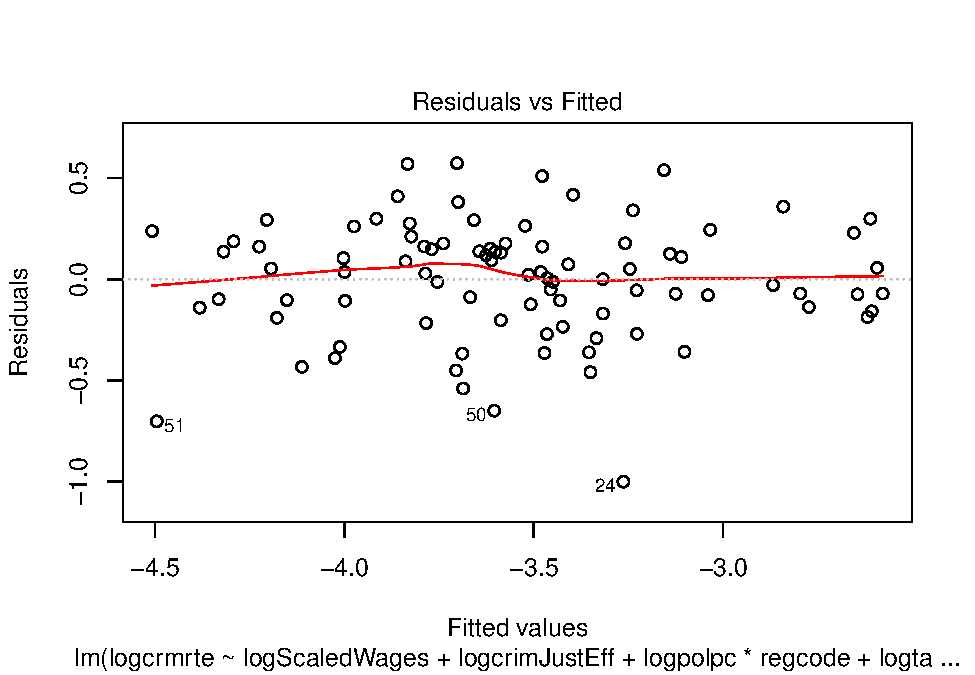
\includegraphics{Bagnard_Gaustad_Hartman_Leung_Lab_3_files/figure-latex/unnamed-chunk-73-1.pdf}

\begin{Shaded}
\begin{Highlighting}[]
\KeywordTok{hist}\NormalTok{(dfCrime}\OperatorTok{$}\NormalTok{allWages)}
\end{Highlighting}
\end{Shaded}

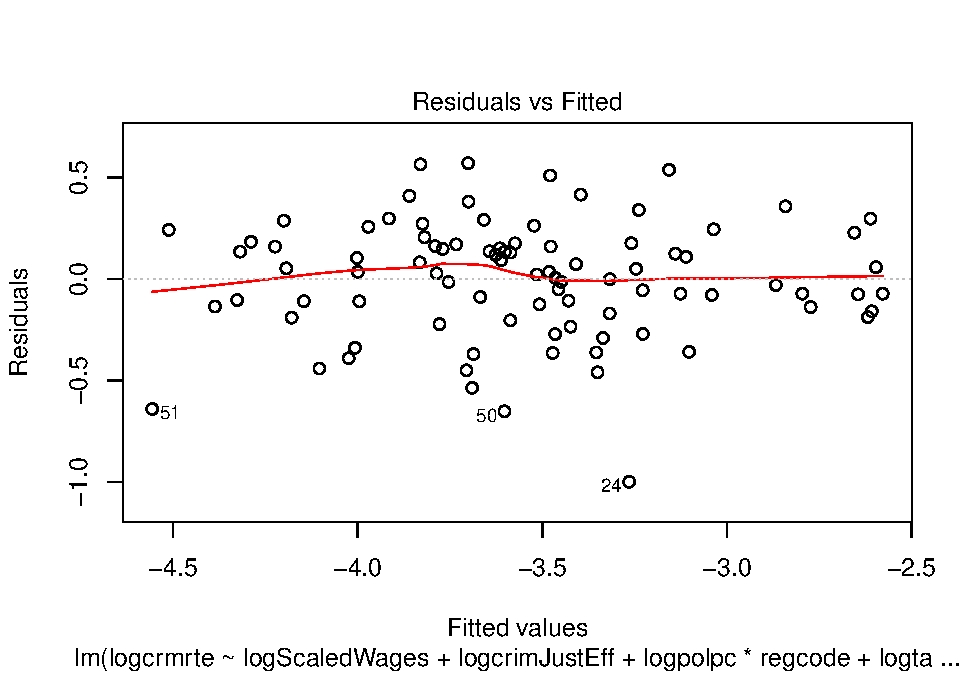
\includegraphics{Bagnard_Gaustad_Hartman_Leung_Lab_3_files/figure-latex/unnamed-chunk-74-1.pdf}

\begin{Shaded}
\begin{Highlighting}[]
\KeywordTok{ggplot}\NormalTok{(}\DataTypeTok{data=}\NormalTok{dfCrime, }\KeywordTok{aes}\NormalTok{(}\DataTypeTok{sample=}\NormalTok{ allWages)) }\OperatorTok{+}\StringTok{ }\KeywordTok{stat_qq}\NormalTok{() }\OperatorTok{+}\StringTok{ }\KeywordTok{stat_qq_line}\NormalTok{() }\OperatorTok{+}
\StringTok{  }\KeywordTok{ggtitle}\NormalTok{(}\StringTok{"QQ Plot of sum of wages"}\NormalTok{)}
\end{Highlighting}
\end{Shaded}

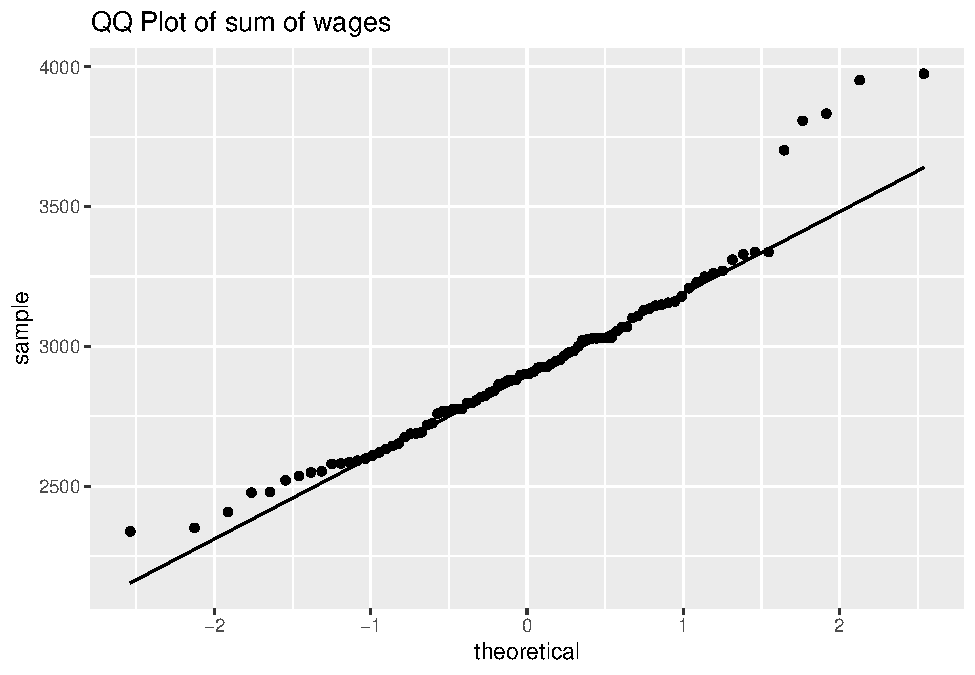
\includegraphics{Bagnard_Gaustad_Hartman_Leung_Lab_3_files/figure-latex/unnamed-chunk-74-2.pdf}

\hypertarget{model-1-linear-model}{%
\subsubsection{Model 1 Linear Model}\label{model-1-linear-model}}

\begin{Shaded}
\begin{Highlighting}[]
\NormalTok{dfCrime}\OperatorTok{$}\NormalTok{unweighted_avg_wage <-}\StringTok{ }\NormalTok{dfCrime}\OperatorTok{$}\NormalTok{allWages}\OperatorTok{/}\DecValTok{9}
\NormalTok{mod1 <-}\StringTok{ }\KeywordTok{lm}\NormalTok{(dfCrime}\OperatorTok{$}\NormalTok{logcrmrte }\OperatorTok{~}\StringTok{ }\NormalTok{dfCrime}\OperatorTok{$}\NormalTok{unweighted_avg_wage }\OperatorTok{+}\StringTok{ }\NormalTok{dfCrime}\OperatorTok{$}\NormalTok{logcrimJustEff)}
\KeywordTok{coeftest}\NormalTok{(mod1, }\DataTypeTok{vcov=}\NormalTok{vcovHC)}
\end{Highlighting}
\end{Shaded}

\begin{verbatim}

t test of coefficients:

                              Estimate Std. Error  t value  Pr(>|t|)    
(Intercept)                 -6.3002758  0.3824297 -16.4743 < 2.2e-16 ***
dfCrime$unweighted_avg_wage  0.0057448  0.0016156   3.5560 0.0006151 ***
dfCrime$logcrimJustEff      -0.4344602  0.1221824  -3.5558 0.0006153 ***
---
Signif. codes:  0 '***' 0.001 '**' 0.01 '*' 0.05 '.' 0.1 ' ' 1
\end{verbatim}

\begin{Shaded}
\begin{Highlighting}[]
\KeywordTok{vif}\NormalTok{(mod1)}
\end{Highlighting}
\end{Shaded}

\begin{verbatim}
dfCrime$unweighted_avg_wage      dfCrime$logcrimJustEff 
                   1.062147                    1.062147 
\end{verbatim}

\begin{Shaded}
\begin{Highlighting}[]
\KeywordTok{summary}\NormalTok{(mod1)}\OperatorTok{$}\NormalTok{adj.r.square}
\end{Highlighting}
\end{Shaded}

\begin{verbatim}
[1] 0.4561573
\end{verbatim}

\begin{Shaded}
\begin{Highlighting}[]
\KeywordTok{shapiro.test}\NormalTok{(mod1}\OperatorTok{$}\NormalTok{residuals)}
\end{Highlighting}
\end{Shaded}

\begin{verbatim}

    Shapiro-Wilk normality test

data:  mod1$residuals
W = 0.97377, p-value = 0.0682
\end{verbatim}

The model gives estimates and standard errors that are heteroskedastic
consistent. The coefficient of unweighted\_avg\_wage is calculated to
have a coefficient of .005. This means that an increase of \$100 in
weekly wages is correlated with an increase of .5\% in crime rate.
Generally increased wages are not associated with increased crime. This
suggests that wages are correlated with a stronger omitted variable that
affects crime.

Similarly, criminal justice effectiveness (convictions/crime) is given a
coefficient of -0.489 which suggests that an increase 1\% increase in
convictions per crime is will decrease crime by nearly .5\%. This
suggests that we have found a are strong correlation and perhaps a good
influence on crime rate in a county.

\begin{Shaded}
\begin{Highlighting}[]
\KeywordTok{plot}\NormalTok{(mod1, }\DataTypeTok{which=}\DecValTok{5}\NormalTok{)}
\end{Highlighting}
\end{Shaded}

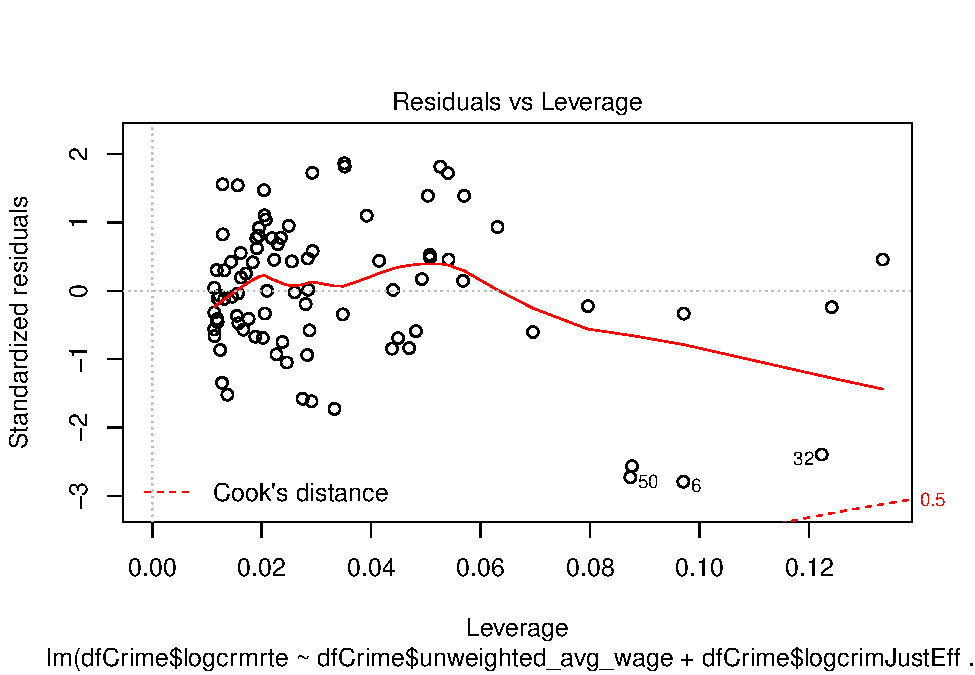
\includegraphics{Bagnard_Gaustad_Hartman_Leung_Lab_3_files/figure-latex/unnamed-chunk-76-1.pdf}

\begin{Shaded}
\begin{Highlighting}[]
\KeywordTok{plot}\NormalTok{(mod1, }\DataTypeTok{which=}\DecValTok{2}\NormalTok{)}
\end{Highlighting}
\end{Shaded}

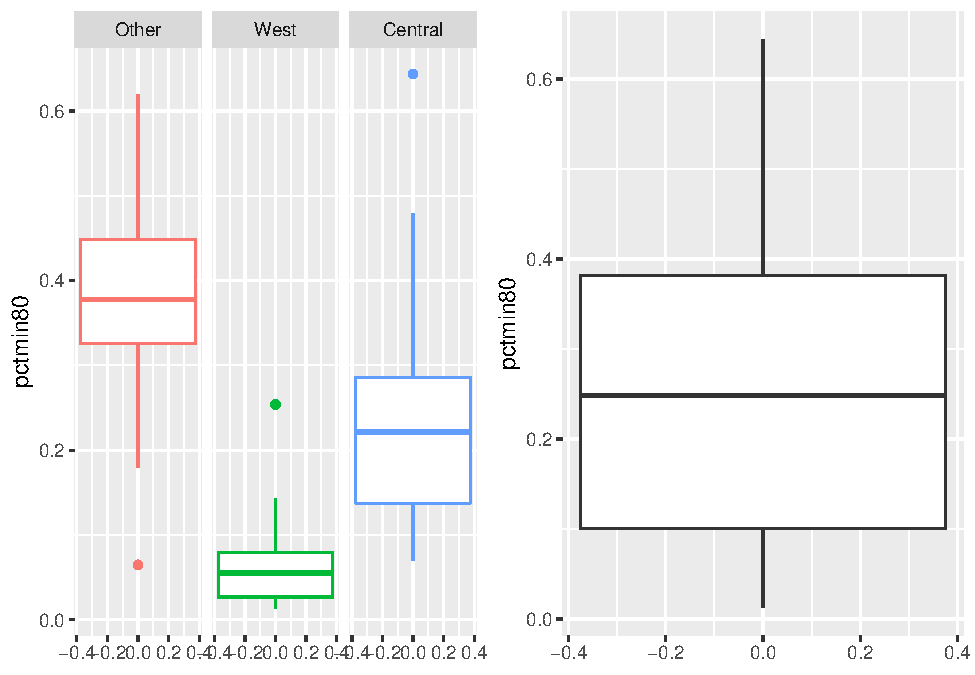
\includegraphics{Bagnard_Gaustad_Hartman_Leung_Lab_3_files/figure-latex/unnamed-chunk-77-1.pdf}

\begin{Shaded}
\begin{Highlighting}[]
\KeywordTok{plot}\NormalTok{(mod1, }\DataTypeTok{which=}\DecValTok{3}\NormalTok{)}
\end{Highlighting}
\end{Shaded}

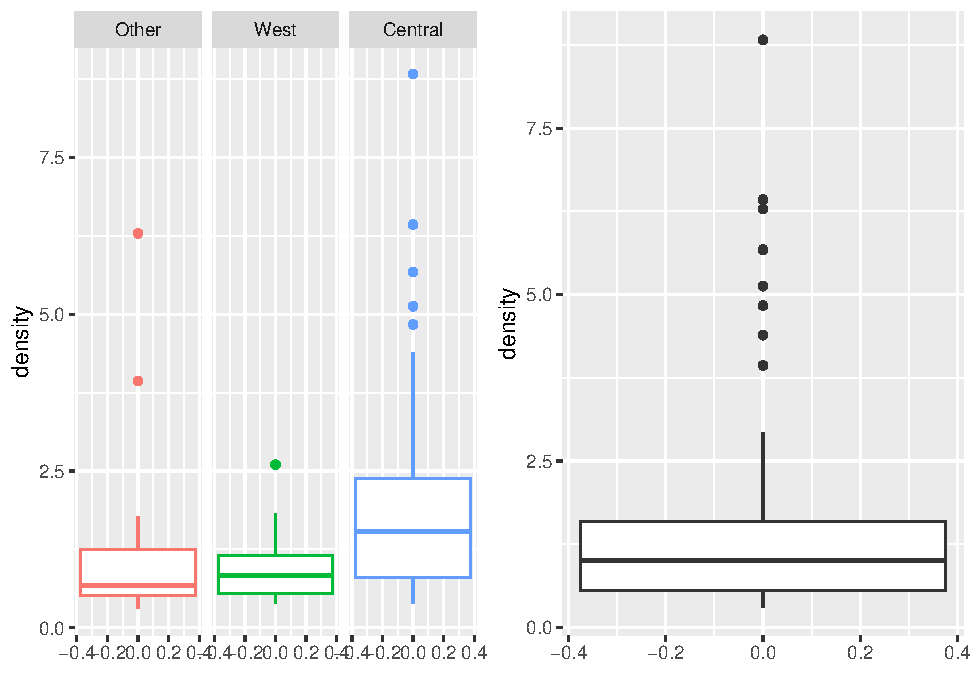
\includegraphics{Bagnard_Gaustad_Hartman_Leung_Lab_3_files/figure-latex/unnamed-chunk-78-1.pdf}

\begin{Shaded}
\begin{Highlighting}[]
\KeywordTok{plot}\NormalTok{(mod1, }\DataTypeTok{which=}\DecValTok{1}\NormalTok{)}
\end{Highlighting}
\end{Shaded}

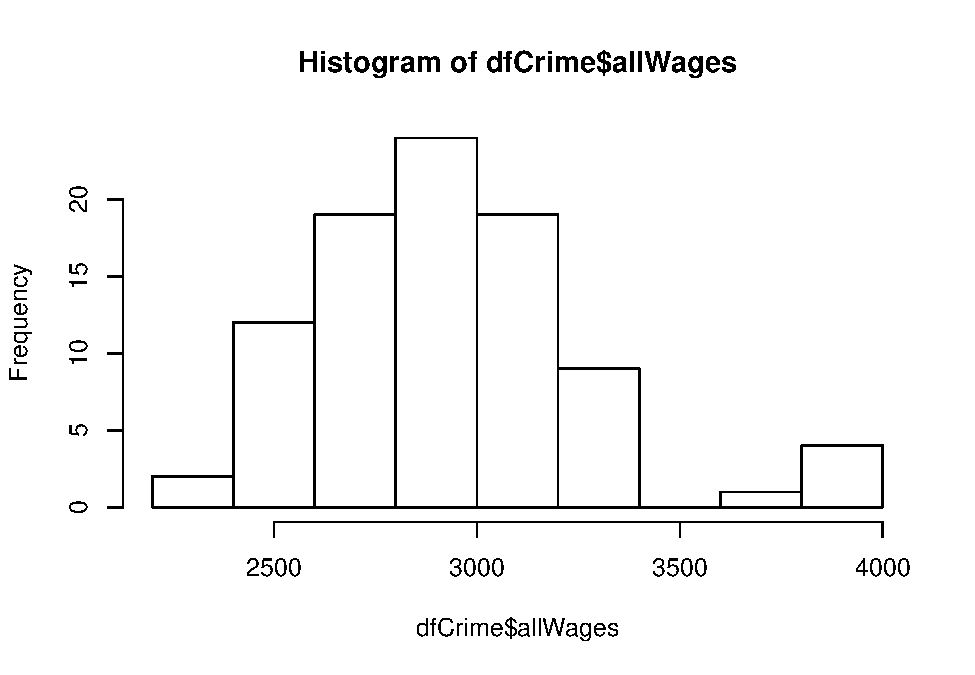
\includegraphics{Bagnard_Gaustad_Hartman_Leung_Lab_3_files/figure-latex/unnamed-chunk-79-1.pdf}

The model shows a moderate good fit, with an adjusted R square of 0.46.
This can be interpreted as, the model explains 46\% of the variation in
crime. Next the model is plotted in a Residuals vs Leverage plot. This
plot shows that all the points have a cook's distance of less than 0.5.
There are no points that have enough leverage and residual than when
deleted greatly alter the model coefficients.

The root of standardized residuals all fall within about 1.6. This is
very good, as we can expect 95\% of the points to fall within 3
standardized residuals of each other. (\(\sqrt(3) \approx 1.73\))

Finally, the residuals vs fitted plot shows a well centered and mostly
nromal distribution about 0. There are no major trends or variation
changes across the fitted values. This suggests that major uncorrelated
variables have not been left out of the model. We will discuss the
possible ommited variable biases further, in the next sections.

\textbf{Model 1 CLM Assumptions: {[}To be finalized{]}} * \textbf{MLR1}
Linear in paramters: The model has had its data transformed as described
above to allow a linear fit of the model. * \textbf{MLR2} Random
Sampling: The data is collected from a data set with rolled up data for
each county. It is not randomly sampled by area or population. *
\textbf{MLR3} No perfect multicollinearity: None of the variables chosen
for the model are constant or perfectly collinear as the economy and
criminal justice effectiveness are independent. * \textbf{MLR4'} The
expectation of u and and covariance of each regressor with u are
\textasciitilde{}0. This shows that our model's regressors are exogenous
with the error.\\
* \textbf{MLR4} The zero conditional mean assumption is well supported
when viewing the Residuals vs fitted plot. The split fit is nearly flat
and centered at 0. * \textbf{MLR5} There does appear to be
heteroskedacity in the `lips' appearance of the Residuals vs fitted
plot. This is acknowledged and can be accounted for by using the
heteroskedastic robust standard errors. This is seen in the coeftest. *
\textbf{MLR6} The final assumption of linear regression is that the
errors are normall distributed. This appears to hold for the bulk of the
residuals with some skewness in the tails. This is shown in the
significant return on the shapiro test. The model should not be used
when predicting crime rate for counties with extreme criminal justice
effectiveness or wages.

To summarize the value of model 1 we found a strong predictor in the
form of criminal justice effectiveness while wages are not good
predictors.

\begin{Shaded}
\begin{Highlighting}[]
\CommentTok{#cov(resid(mod1), dfCrime$allWages)}
\CommentTok{#cov(resid(mod1), log(dfCrime$crimJustEff))}
\KeywordTok{mean}\NormalTok{(}\KeywordTok{resid}\NormalTok{(mod1))}
\end{Highlighting}
\end{Shaded}

\begin{verbatim}
[1] -5.23828e-18
\end{verbatim}

\hypertarget{model-2}{%
\subsection{Model 2}\label{model-2}}

\hypertarget{introduction-2}{%
\subsubsection{Introduction}\label{introduction-2}}

In this model, we introduce the additional covariates of population per
square mile (density), tax per capita (taxpc) and police per capita
(polpc) to increase the accuracy of our regression. We are including
these additional variables to our second model, as they add accuracy to
the explanatory variables used in our first model:

\begin{enumerate}
\def\labelenumi{\arabic{enumi}.}
\tightlist
\item
  The \textbf{Density} of an area can have significant impacts on:

  \begin{itemize}
  \tightlist
  \item
    \textbf{Criminal Justice Effectiveness}: with more people in a given
    area, crime frequency increases (+ bias direction). However, more
    people means there are more potential witnesses, making it easier to
    catch criminals (- bias direction).
  \item
    \textbf{Economic Opportunity (ie. AllWages)}: in high density areas,
    there is an increase in demand for support services such as food,
    retail, utilities, etc. As a result, there is a high demand for
    service jobs, which increases the economic opportunities within the
    area (+ bias direction). However, more people in a given area, there
    is a closer proximity to drugs, alcohol and gang violence - all of
    which are inhimitors to better economic outcomes.
  \end{itemize}
\item
  The \textbf{Police Per Capita} in a county can be influential on the
  Criminal Justice Effectiveness. With more police in a given area, one
  would think that crime rates would decrease, however our correlation
  plot below tells a different story. Including this variable in our
  analysis will give us more insight into the variables used in model 1.
\item
  The \textbf{Tax Per Capita} can have a direct impact on the Police Per
  Capita. A higher tax per capita, means that the county has more tax
  dollars to spend on protection services (ie. increasing the number of
  police in the county).
\end{enumerate}

\[log(crmrate) = \beta_0 + \beta_1crimjusteff + \beta_2log(polpc) + \beta_3density + \beta_4allWages + \beta_5taxpc + u\]

\hypertarget{model-2-eda-and-data-transformations}{%
\subsubsection{Model 2 EDA and Data
Transformations}\label{model-2-eda-and-data-transformations}}

\begin{Shaded}
\begin{Highlighting}[]
\KeywordTok{corrplot}\NormalTok{(}\KeywordTok{cor}\NormalTok{(dfCrime[,}\KeywordTok{c}\NormalTok{(}\StringTok{"logcrmrte"}\NormalTok{, }\StringTok{"logcrimJustEff"}\NormalTok{, }\StringTok{"logprbarr"}\NormalTok{, }\StringTok{"logprbconv"}\NormalTok{, }
                        \StringTok{"prbpris"}\NormalTok{, }\StringTok{"polpc"}\NormalTok{, }\StringTok{"taxpc"}\NormalTok{, }\StringTok{"allWages"}\NormalTok{, }\StringTok{"urban"}\NormalTok{, }\StringTok{"density"}\NormalTok{,}
                        \StringTok{"pctymle"}\NormalTok{, }\StringTok{"pctmin80"}\NormalTok{)]),}\DataTypeTok{method=}\StringTok{'circle'}\NormalTok{, }\DataTypeTok{type =} \StringTok{'lower'}\NormalTok{)}
\end{Highlighting}
\end{Shaded}

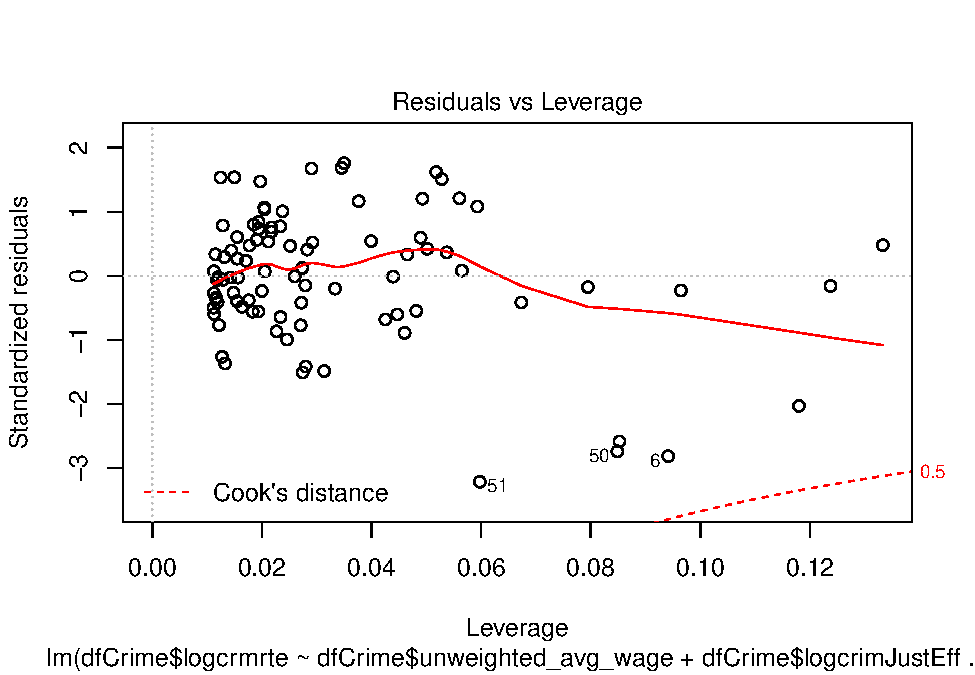
\includegraphics{Bagnard_Gaustad_Hartman_Leung_Lab_3_files/figure-latex/unnamed-chunk-81-1.pdf}

\begin{Shaded}
\begin{Highlighting}[]
\CommentTok{# polpc transformation analysis }
\KeywordTok{par}\NormalTok{(}\DataTypeTok{mfrow =} \KeywordTok{c}\NormalTok{(}\DecValTok{2}\NormalTok{,}\DecValTok{2}\NormalTok{))}
\KeywordTok{hist}\NormalTok{(dfCrime}\OperatorTok{$}\NormalTok{polpc, }\DataTypeTok{main=}\StringTok{"Hist of polpc"}\NormalTok{, }\DataTypeTok{breaks=}\DecValTok{50}\NormalTok{)}
\KeywordTok{hist}\NormalTok{(dfCrime}\OperatorTok{$}\NormalTok{logpolpc, }\DataTypeTok{main=}\StringTok{"Hist of logpolpc"}\NormalTok{, }\DataTypeTok{breaks=}\DecValTok{50}\NormalTok{)}
\KeywordTok{hist}\NormalTok{(}\DecValTok{1}\OperatorTok{/}\NormalTok{dfCrime}\OperatorTok{$}\NormalTok{polpc, }\DataTypeTok{main=}\StringTok{"Hist of Recip polpc"}\NormalTok{, }\DataTypeTok{breaks=}\DecValTok{50}\NormalTok{)}
\KeywordTok{hist}\NormalTok{(}\KeywordTok{sqrt}\NormalTok{(dfCrime}\OperatorTok{$}\NormalTok{polpc), }\DataTypeTok{main=}\StringTok{"Hist of Sqrt polpc"}\NormalTok{, }\DataTypeTok{breaks=}\DecValTok{50}\NormalTok{)}
\end{Highlighting}
\end{Shaded}

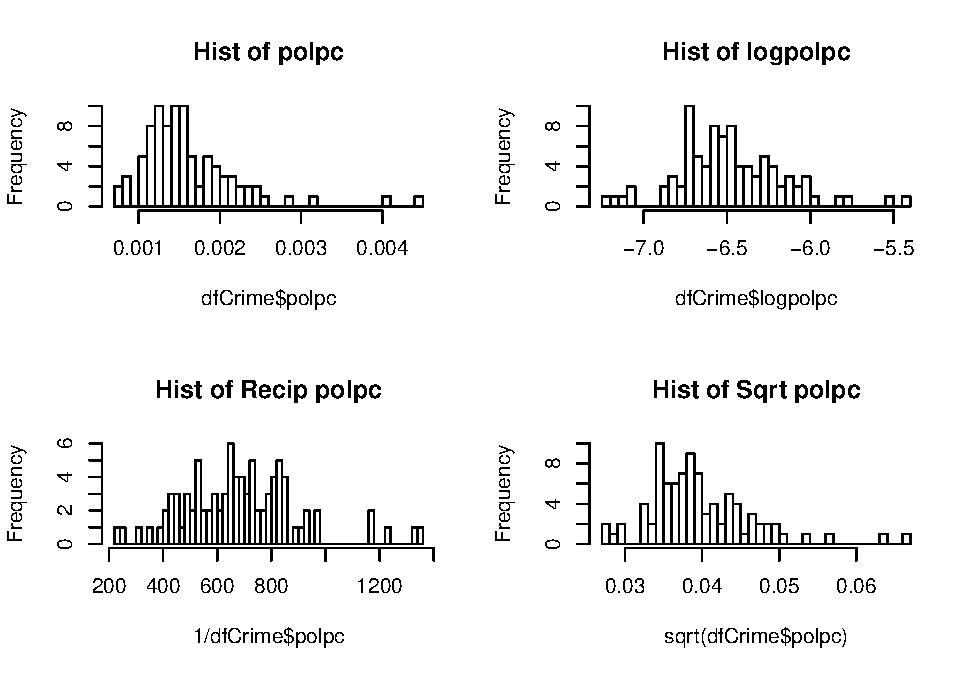
\includegraphics{Bagnard_Gaustad_Hartman_Leung_Lab_3_files/figure-latex/unnamed-chunk-82-1.pdf}

\begin{Shaded}
\begin{Highlighting}[]
\CommentTok{# taxpc transformation analysis }
\KeywordTok{par}\NormalTok{(}\DataTypeTok{mfrow =} \KeywordTok{c}\NormalTok{(}\DecValTok{2}\NormalTok{,}\DecValTok{2}\NormalTok{))}
\KeywordTok{hist}\NormalTok{(dfCrime}\OperatorTok{$}\NormalTok{taxpc, }\DataTypeTok{main=}\StringTok{"Hist of taxpc"}\NormalTok{, }\DataTypeTok{breaks=}\DecValTok{50}\NormalTok{)}
\KeywordTok{hist}\NormalTok{(dfCrime}\OperatorTok{$}\NormalTok{logtaxpc, }\DataTypeTok{main=}\StringTok{"Hist of logtaxpc"}\NormalTok{,}\DataTypeTok{breaks=}\DecValTok{50}\NormalTok{)}
\KeywordTok{hist}\NormalTok{(}\DecValTok{1}\OperatorTok{/}\NormalTok{dfCrime}\OperatorTok{$}\NormalTok{taxpc, }\DataTypeTok{main=}\StringTok{"Hist of Recip taxpc"}\NormalTok{, }\DataTypeTok{breaks=}\DecValTok{50}\NormalTok{)}
\KeywordTok{hist}\NormalTok{(}\KeywordTok{sqrt}\NormalTok{(dfCrime}\OperatorTok{$}\NormalTok{taxpc), }\DataTypeTok{main=}\StringTok{"Hist of Sqrt taxpc"}\NormalTok{, }\DataTypeTok{breaks=}\DecValTok{50}\NormalTok{)}
\end{Highlighting}
\end{Shaded}

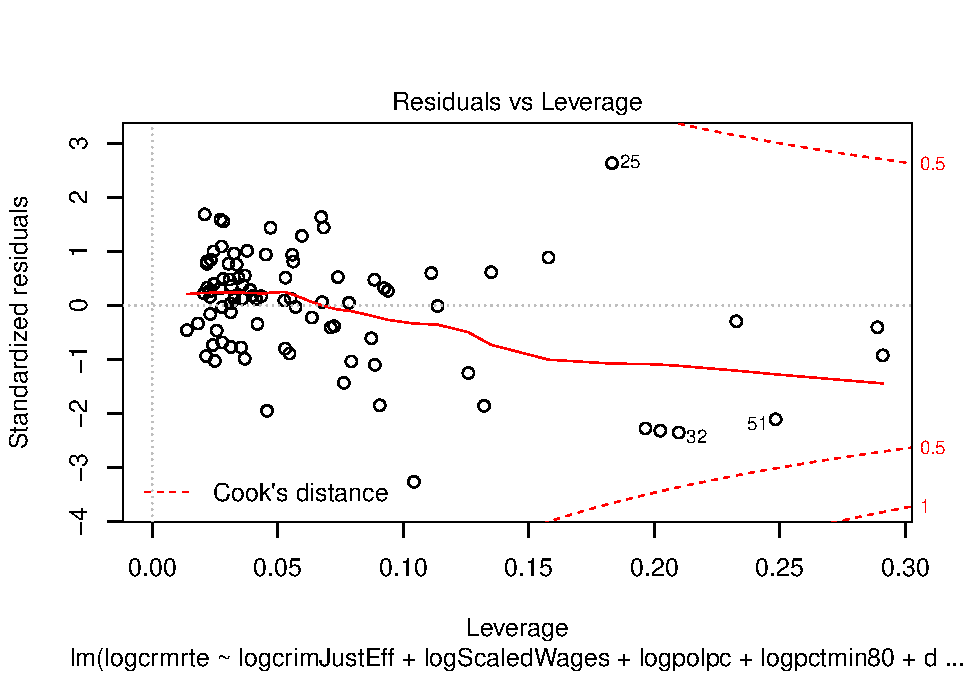
\includegraphics{Bagnard_Gaustad_Hartman_Leung_Lab_3_files/figure-latex/unnamed-chunk-83-1.pdf}

\begin{Shaded}
\begin{Highlighting}[]
\CommentTok{# density transformation analysis }
\KeywordTok{par}\NormalTok{(}\DataTypeTok{mfrow =} \KeywordTok{c}\NormalTok{(}\DecValTok{2}\NormalTok{,}\DecValTok{2}\NormalTok{))}
\KeywordTok{hist}\NormalTok{(dfCrime}\OperatorTok{$}\NormalTok{density, }\DataTypeTok{main=}\StringTok{"Hist of density"}\NormalTok{, }\DataTypeTok{breaks=}\DecValTok{50}\NormalTok{)}
\KeywordTok{hist}\NormalTok{(dfCrime}\OperatorTok{$}\NormalTok{logdensity, }\DataTypeTok{main=}\StringTok{"Hist of logdensity"}\NormalTok{,}\DataTypeTok{breaks=}\DecValTok{50}\NormalTok{)}
\KeywordTok{hist}\NormalTok{(}\DecValTok{1}\OperatorTok{/}\NormalTok{dfCrime}\OperatorTok{$}\NormalTok{density, }\DataTypeTok{main=}\StringTok{"Hist of Recip density"}\NormalTok{, }\DataTypeTok{breaks=}\DecValTok{50}\NormalTok{)}
\KeywordTok{hist}\NormalTok{(}\KeywordTok{sqrt}\NormalTok{(dfCrime}\OperatorTok{$}\NormalTok{density), }\DataTypeTok{main=}\StringTok{"Hist of Sqrt density"}\NormalTok{, }\DataTypeTok{breaks=}\DecValTok{50}\NormalTok{)}
\end{Highlighting}
\end{Shaded}

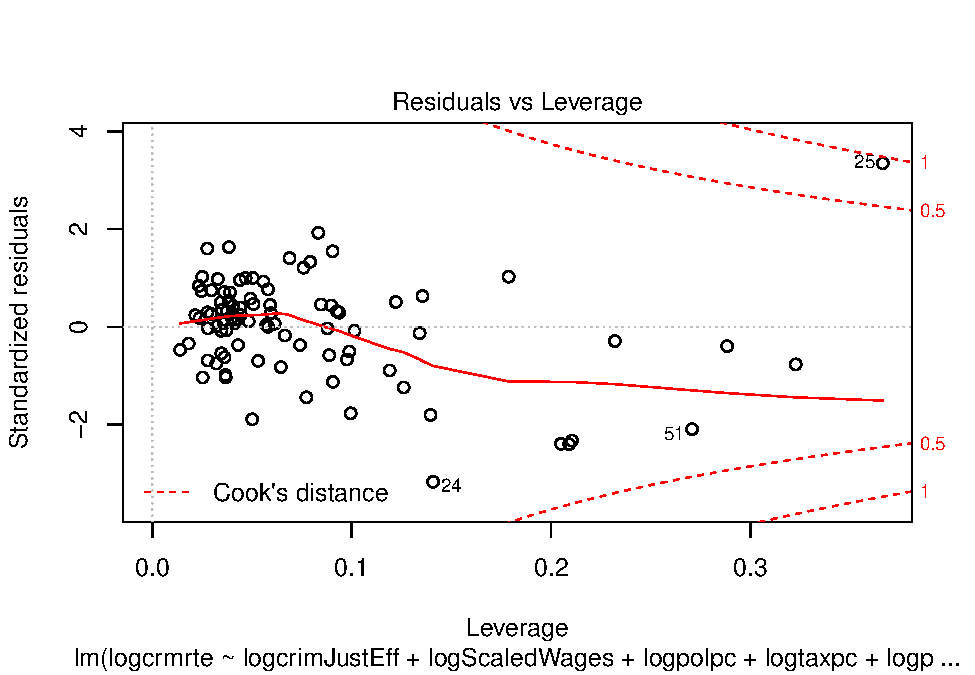
\includegraphics{Bagnard_Gaustad_Hartman_Leung_Lab_3_files/figure-latex/unnamed-chunk-84-1.pdf}

\begin{Shaded}
\begin{Highlighting}[]
\CommentTok{# par(mfrow = c(2,2))}
\CommentTok{# plot(dfCrime$logcrimJustEff, dfCrime$polpc, main = 'polpc vs logcrimJustEff', xlab='logcrimJustEff', ylab='polpc')}
\CommentTok{# plot(dfCrime$logcrimJustEff, dfCrime$logpolpc, main = 'logpolpc vs logcrimJustEff', xlab='logcrimJustEff', ylab='logpolpc')}
\CommentTok{# plot(dfCrime$logcrimJustEff, dfCrime$taxpc, main = 'taxpc vs logcrimJustEff', xlab='logcrimJustEff', ylab='taxpc')}
\CommentTok{# plot(dfCrime$logcrimJustEff, dfCrime$logtaxpc, main = 'logtaxpc vs logcrimJustEff', xlab='logcrimJustEff', ylab='logtaxpc')}
\end{Highlighting}
\end{Shaded}

-- AXLB - WIP

In the histograms above, we see that the both polpc and taxpc exhibit
right skew. Taking the natural log of polpc brings the distribution
closer to normal. However, the \(log\) of taxpc and density makes the
distributions even more skewed.

As a result, we will use the \(log\) of polpc (logpolpc) in our second
model and will not transform the taxpc and density variables.

\hypertarget{model-2-linear-model}{%
\subsubsection{Model 2 Linear Model}\label{model-2-linear-model}}

\begin{Shaded}
\begin{Highlighting}[]
\NormalTok{model2 <-}\StringTok{ }\KeywordTok{lm}\NormalTok{(logcrmrte }\OperatorTok{~}\StringTok{ }\NormalTok{logcrimJustEff }\OperatorTok{+}\StringTok{ }\NormalTok{logpolpc }\OperatorTok{+}\StringTok{ }\KeywordTok{log}\NormalTok{(allWages) }\OperatorTok{+}\StringTok{ }\NormalTok{logtaxpc }\OperatorTok{+}\StringTok{ }\KeywordTok{sqrt}\NormalTok{(dfCrime}\OperatorTok{$}\NormalTok{density), }\DataTypeTok{data =}\NormalTok{ dfCrime)}
\NormalTok{model2}
\end{Highlighting}
\end{Shaded}

\begin{verbatim}

Call:
lm(formula = logcrmrte ~ logcrimJustEff + logpolpc + log(allWages) + 
    logtaxpc + sqrt(dfCrime$density), data = dfCrime)

Coefficients:
          (Intercept)         logcrimJustEff               logpolpc  
             -6.47921               -0.25967                0.33279  
        log(allWages)               logtaxpc  sqrt(dfCrime$density)  
              0.50075                0.03552                0.40521  
\end{verbatim}

-- cooks distance analysis --

\textbf{Model 2 CLM Assumptions:}

\begin{itemize}
\item
  \textbf{MLR1} Discussed above.
\item
  \textbf{MLR2} Discussed above.
\item
  \textbf{MLR3: Non-perfect Collinearity} We will use the VIF function
  to provide evidence that our variables in model2 are not perfectly
  multicollinear. As we can see from the VIF results, below, all of the
  variables' values are less than five, which allows us to conclude
  model2 is free from multicollinearity.
\end{itemize}

\begin{Shaded}
\begin{Highlighting}[]
\KeywordTok{vif}\NormalTok{(model2)}
\end{Highlighting}
\end{Shaded}

\begin{verbatim}
##        logcrimJustEff              logpolpc         log(allWages) 
##              1.378627              1.663614              2.006571 
##              logtaxpc sqrt(dfCrime$density) 
##              1.358061              2.385209
\end{verbatim}

\begin{itemize}
\tightlist
\item
  \textbf{MLR4: Zero Conditional Mean} The residual vs.~fitted chart,
  below, gives us evidence that we meet the zero conditional mean
  assumption as the majority of the residual means lie close to zero.
  The exceptions to this trend, lie on the right side of the chart where
  there are fewer data points (evidence for heteroscedasticity - see
  MLR5, below).
\end{itemize}

\begin{Shaded}
\begin{Highlighting}[]
\KeywordTok{plot}\NormalTok{(model2, }\DataTypeTok{which=}\DecValTok{1}\NormalTok{)}
\end{Highlighting}
\end{Shaded}

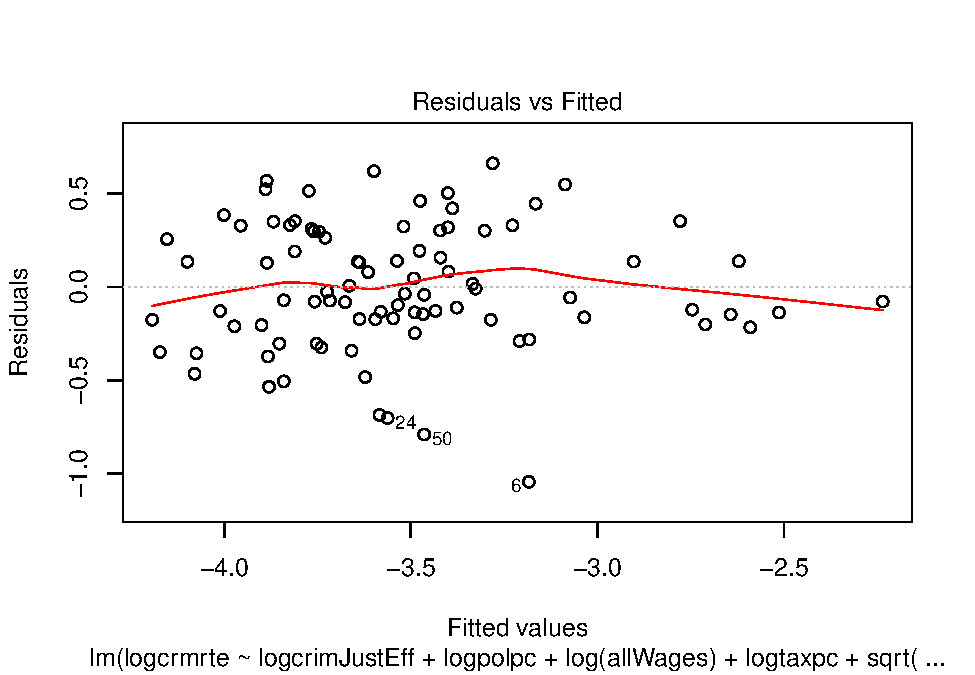
\includegraphics{Bagnard_Gaustad_Hartman_Leung_Lab_3_files/figure-latex/unnamed-chunk-88-1.pdf}

\begin{itemize}
\tightlist
\item
  \textbf{MLR5: Homoscedasticity} The above Residuals vs Fitted graph
  provides evidence of heteroscedasticity as right side of the chart
  have fewer datepoints. To provide further evidence of
  heteroscedasticity, we will use the White test to generate
  coefficients with robust with vcovHC
\end{itemize}

non-significan coeffs (pr(\textgreater{}t)) \textgreater{}
.05\ldots{}make a model to remove all the non-significant and then
analyze using the f-test.

-- AXLB - WIP

\begin{Shaded}
\begin{Highlighting}[]
\KeywordTok{coeftest}\NormalTok{(model2, }\DataTypeTok{vcov=}\NormalTok{vcovHC)}
\end{Highlighting}
\end{Shaded}

\begin{verbatim}

t test of coefficients:

                       Estimate Std. Error t value Pr(>|t|)   
(Intercept)           -6.479213   5.863983 -1.1049 0.272388   
logcrimJustEff        -0.259675   0.125841 -2.0635 0.042189 * 
logpolpc               0.332786   0.233732  1.4238 0.158255   
log(allWages)          0.500752   0.596805  0.8391 0.403849   
logtaxpc               0.035525   0.231771  0.1533 0.878553   
sqrt(dfCrime$density)  0.405213   0.133994  3.0241 0.003318 **
---
Signif. codes:  0 '***' 0.001 '**' 0.01 '*' 0.05 '.' 0.1 ' ' 1
\end{verbatim}

\begin{itemize}
\tightlist
\item
  \textbf{MLR6: Normal Distribution of Errors} The Normal Q-Q plot,
  below, provides evidence that our residuals follow a normal
  distribution. While there are some data points on the left and right
  side of the graph that stray from the diagonal line, since our data
  set has over 30 datapoints, per the CLT, we can assume residuals have
  a normal distribution.
\end{itemize}

\begin{Shaded}
\begin{Highlighting}[]
\KeywordTok{plot}\NormalTok{(model2, }\DataTypeTok{which=}\DecValTok{2}\NormalTok{)}
\end{Highlighting}
\end{Shaded}

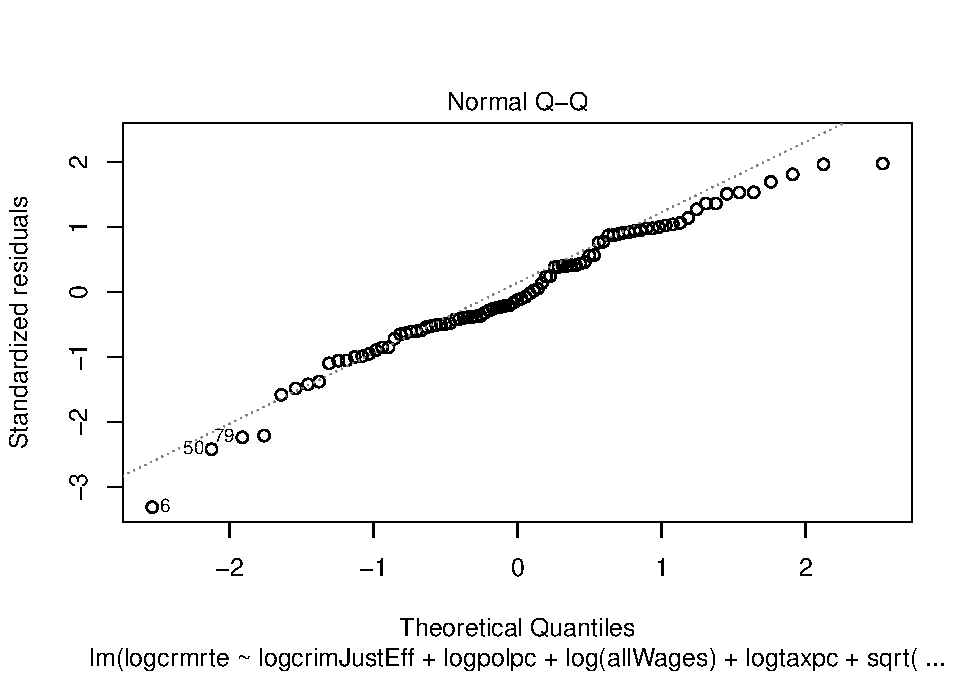
\includegraphics{Bagnard_Gaustad_Hartman_Leung_Lab_3_files/figure-latex/unnamed-chunk-90-1.pdf}

\begin{Shaded}
\begin{Highlighting}[]
\CommentTok{# hist(model2$residuals)}
\CommentTok{# shapiro.test(model2$residuals)}
\CommentTok{#null hypothesis: residuals drawn from population with a normal distribution. }
\CommentTok{#small p-value tells you if you can reject the null hypothesis. }
\CommentTok{#this test depends on sample size, it does not take very much deviation from normality for}
\CommentTok{#us to get a statistically significant result}
\end{Highlighting}
\end{Shaded}

\begin{Shaded}
\begin{Highlighting}[]
\KeywordTok{summary}\NormalTok{(model2)}
\end{Highlighting}
\end{Shaded}

\begin{verbatim}
## 
## Call:
## lm(formula = logcrmrte ~ logcrimJustEff + logpolpc + log(allWages) + 
##     logtaxpc + sqrt(dfCrime$density), data = dfCrime)
## 
## Residuals:
##      Min       1Q   Median       3Q      Max 
## -1.04290 -0.17570 -0.04186  0.29765  0.66230 
## 
## Coefficients:
##                       Estimate Std. Error t value Pr(>|t|)    
## (Intercept)           -6.47921    4.09171  -1.583 0.117112    
## logcrimJustEff        -0.25967    0.07743  -3.354 0.001203 ** 
## logpolpc               0.33279    0.14594   2.280 0.025150 *  
## log(allWages)          0.50075    0.48309   1.037 0.302949    
## logtaxpc               0.03552    0.16220   0.219 0.827177    
## sqrt(dfCrime$density)  0.40521    0.11631   3.484 0.000792 ***
## ---
## Signif. codes:  0 '***' 0.001 '**' 0.01 '*' 0.05 '.' 0.1 ' ' 1
## 
## Residual standard error: 0.346 on 83 degrees of freedom
##   (1 observation deleted due to missingness)
## Multiple R-squared:  0.5864, Adjusted R-squared:  0.5615 
## F-statistic: 23.53 on 5 and 83 DF,  p-value: 1.189e-14
\end{verbatim}

The Adjusted R-squared variable penalizes for additional variables,
which means there is a chance that this value will decrease if the added
variables do not contribute to the model. By comparing the Adjusted
R-squared value between our first and second models, we see that
log(polpc), taxpc and density help describe log(crmrate). Our second
model has an Adjusted R-squared value of 0.5004, which means 50.04\% of
the variation in the \(log_{10}\) of crime rate is explained by the
explanatory variables used in this model. This is a significant increase
compared to our first model, that has an Adjusted R-squared value of
0.4520.

In addition, the F-statistic is 16.62 with a statistically significant
p-value of \textless{} 6.263e-11. As a result, we reject the null
hypothesis that none of the independent variables help to describe
log(crmrate).

Coefficient Analysis (assuming ceterus paribus): - logcrimJustEff:
-0.1607. This suggests that for a 1\% increase in criminal justice
efficiency, there is a 0.1607\% decrease in crime rate. - logpolpc:
0.3701. This suggests that for a 1\% increase in police per capita,
there is a 0.3701\% increase in crime rate. - allWages: 0.00006692. This
suggests that for a 1\% increase in total average weekly wage, there is
a 0.0067\% increase in crime rate. - taxpc: -0.001632. This suggests
that for a 1\% increase in tax per capita, there is a 0.1632\% decrease
in crime rate. - density: 0.06259. This suggests that for a 1\% increase
in density, there is a 6.259\% increase in crime rate.

\hypertarget{conclusion-are-the-conclusions-they-draw-based-on-this-evaluation-appropriate-did-the-team-interpret-the-results-in-terms-of-their-research-question}{%
\subsubsection{Conclusion : Are the conclusions they draw based on this
evaluation appropriate? Did the team interpret the results in terms of
their research
question?}\label{conclusion-are-the-conclusions-they-draw-based-on-this-evaluation-appropriate-did-the-team-interpret-the-results-in-terms-of-their-research-question}}

Compared to model 1, the adjusted \(R^2\) of model 2 is only marginally
higher. This suggests that we should continue our analysis by focusing
on the join significance of the variables added in model 2.

\hypertarget{model-3}{%
\subsection{Model 3}\label{model-3}}

\hypertarget{discussion-of-variables}{%
\subsubsection{Discussion of Variables}\label{discussion-of-variables}}

Despite the improvements in the accuracy of model 2 over model 1, we are
still only explaining about 55\% of the variation in our data. As a
result, we propose to also analyse the topic of demographics which could
have an effect on both of our key explanatory variables.

One key component of demographics is the race of the county inhabitants
and how they are perceived and treated by others, especially for
minorities in the population. For example, systemic racism could have an
important effect on: * Criminal Justice Effectiveness: If police,
lawyers and judges are racially biased, this could lead to more arrests
and more convictions regardless of the strength of the legal case and
the evidence. As a result, we hypothesize the crime rate would increase.
* Economic Opportunity: Racism could prohibit members of the minority
from having access to education, jobs and higher wages. Racism could
also limit access to healthcare and social programmes which has a
negative effect on economic opportunity.

However, since we cannot directly measure racism, we have to
operationalize this covariate by examining its effect in the real world.
We propose to use the variable pctmin80, which represents the percentage
of minorities in the population of the county. This is also a continous
parameter and so given a higher the percentage of minorities, we should
expect to see a greater effect.

From the summary and boxplot below, we can see that the percentage of
minorities ranges from 0.0154 - 0.6435, with a mean of 0.2621. We note
that there are no major outliers. We will apply the natural log to the
variable pctmin80 to 1) make it easier for us to interpret the
coefficient in our linear model and 2) to better expose the linear
relationship in the model.

\begin{Shaded}
\begin{Highlighting}[]
\KeywordTok{summary}\NormalTok{(dfCrime}\OperatorTok{$}\NormalTok{pctmin80)}
\end{Highlighting}
\end{Shaded}

\begin{verbatim}
   Min. 1st Qu.  Median    Mean 3rd Qu.    Max. 
0.01284 0.10024 0.24852 0.25713 0.38183 0.64348 
\end{verbatim}

\begin{Shaded}
\begin{Highlighting}[]
\KeywordTok{boxplot}\NormalTok{(dfCrime}\OperatorTok{$}\NormalTok{pctmin80)}
\end{Highlighting}
\end{Shaded}

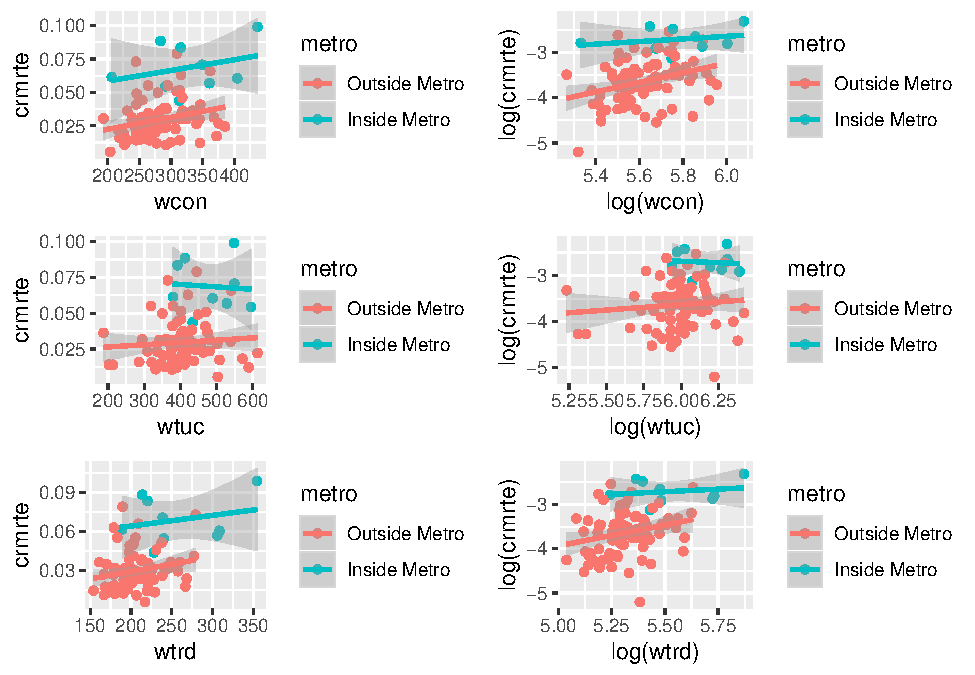
\includegraphics{Bagnard_Gaustad_Hartman_Leung_Lab_3_files/figure-latex/unnamed-chunk-92-1.pdf}

In addition, we hypothesize that the location of the county can have an
impact on demographcs. We can see that counties in the West have a
significantly lower percentage of minorities than the other two regions.
As a result, we will also test for region in our model.

\begin{Shaded}
\begin{Highlighting}[]
\KeywordTok{ggplot}\NormalTok{(}\DataTypeTok{data =}\NormalTok{ dfCrime, }\KeywordTok{aes}\NormalTok{(}\DataTypeTok{y =}\NormalTok{ pctmin80, }\DataTypeTok{color=}\NormalTok{regcode)) }\OperatorTok{+}\StringTok{ }
\StringTok{      }\KeywordTok{geom_boxplot}\NormalTok{() }\OperatorTok{+}\StringTok{ }\KeywordTok{ggtitle}\NormalTok{(}\StringTok{"Percentage of minorities in the County by Region"}\NormalTok{)}
\end{Highlighting}
\end{Shaded}

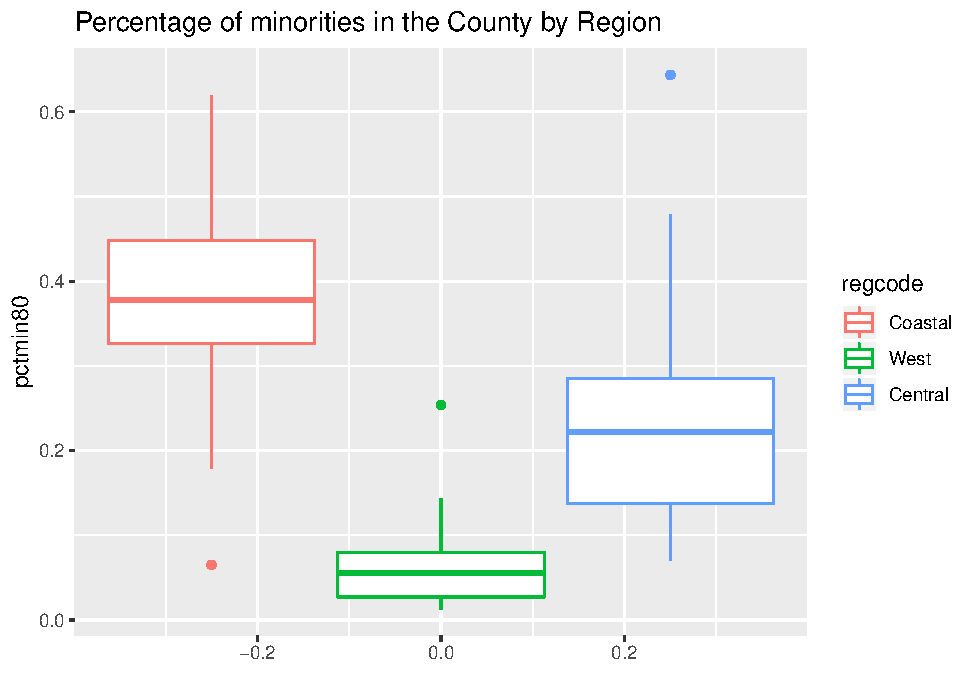
\includegraphics{Bagnard_Gaustad_Hartman_Leung_Lab_3_files/figure-latex/unnamed-chunk-93-1.pdf}
\textbf{UPDATE AFTER ALEXA} Given that our analysis of model 2 showed
that taxpc was not statistically significant, we will not consider it in
our model.

We have also chosen not to include other variables from our dataset in
our model: * Urban: We believe the variable ``density'' better explains
the same effects as ``urban'', while also being a linear parameter. In
addition, there may be data points that failed to meet the cutoff for
being defined as urban, but may still see the same effects as being
urban and hence may distort our analysis. * Age and Gender: While age
and gender are important demographic variables, the only variable in our
dataset is pctymle which provides the percentage of young males in the
population. However, given that this variable encompasses both male and
young, we may not be able to discern if age or gender has the larger
effect (if any at all). * Judgement: We chose not to include the
varibles concerning the probability of a prison sentence as well as the
average sentence as we believe it is unlikely that potential criminals
would have good access to this information. In addition, local county
officials have limited influence over the decisions of the judiciary
system, as they are separate branches of government.

Our equation for model 3 is as follows:
\[log(crmrate) = \beta_0 + \beta_1log(crimjusteff) + \beta_2log(polpc) + \beta_3density + \beta_4log(allWages) + \beta_5logpctmin80 + \beta_6west + \beta_7central+u\]

\hypertarget{model-3-linear-model}{%
\subsubsection{Model 3 Linear Model}\label{model-3-linear-model}}

\begin{Shaded}
\begin{Highlighting}[]
\NormalTok{dfCrime}\OperatorTok{$}\NormalTok{logunweightedavg<-}\KeywordTok{log}\NormalTok{(dfCrime}\OperatorTok{$}\NormalTok{unweighted_avg_wage)}
\NormalTok{model3_initial<-}\KeywordTok{lm}\NormalTok{(logcrmrte }\OperatorTok{~}\StringTok{ }\NormalTok{logcrimJustEff }\OperatorTok{+}\StringTok{ }\NormalTok{logpolpc }\OperatorTok{+}\StringTok{ }\NormalTok{logunweightedavg }\OperatorTok{+}\StringTok{  }\NormalTok{density }\OperatorTok{+}\StringTok{ }\NormalTok{logpctmin80 }\OperatorTok{+}\StringTok{ }\NormalTok{west }\OperatorTok{+}\StringTok{ }\NormalTok{central, }\DataTypeTok{data =}\NormalTok{ dfCrime)}
\KeywordTok{summary}\NormalTok{(model3_initial)}
\end{Highlighting}
\end{Shaded}

\begin{verbatim}

Call:
lm(formula = logcrmrte ~ logcrimJustEff + logpolpc + logunweightedavg + 
    density + logpctmin80 + west + central, data = dfCrime)

Residuals:
     Min       1Q   Median       3Q      Max 
-0.88805 -0.14672  0.05094  0.14252  0.59964 

Coefficients:
                 Estimate Std. Error t value Pr(>|t|)    
(Intercept)      -8.25258    2.41603  -3.416 0.000997 ***
logcrimJustEff   -0.34825    0.06551  -5.316 9.17e-07 ***
logpolpc          0.33920    0.10682   3.175 0.002117 ** 
logunweightedavg  1.11492    0.37410   2.980 0.003801 ** 
density           0.08362    0.02842   2.943 0.004241 ** 
logpctmin80       0.14324    0.05640   2.539 0.013015 *  
west             -0.26442    0.13219  -2.000 0.048807 *  
central          -0.17853    0.07786  -2.293 0.024448 *  
---
Signif. codes:  0 '***' 0.001 '**' 0.01 '*' 0.05 '.' 0.1 ' ' 1

Residual standard error: 0.2749 on 81 degrees of freedom
  (1 observation deleted due to missingness)
Multiple R-squared:  0.7452,    Adjusted R-squared:  0.7231 
F-statistic: 33.84 on 7 and 81 DF,  p-value: < 2.2e-16
\end{verbatim}

We note from the two F-tests below that west and central were not
statistically significant to the model, but the inclusion of logpctmin80
is highly significant. An analysis of VIF(model3) also indicates that
logpctmin80 and west have higher variance inflation factors as compared
to the others. It appears then that logpctmin80 better explains the
difference in demographics than west or central, and we thus remove the
latter 2 variables from our model.

\begin{Shaded}
\begin{Highlighting}[]
\KeywordTok{linearHypothesis}\NormalTok{(model3_initial,}\KeywordTok{c}\NormalTok{(}\StringTok{"west=0"}\NormalTok{,}\StringTok{"central=0"}\NormalTok{), }\DataTypeTok{vcov=}\NormalTok{vcovHC)}
\end{Highlighting}
\end{Shaded}

\begin{verbatim}
## Linear hypothesis test
## 
## Hypothesis:
## west = 0
## central = 0
## 
## Model 1: restricted model
## Model 2: logcrmrte ~ logcrimJustEff + logpolpc + logunweightedavg + density + 
##     logpctmin80 + west + central
## 
## Note: Coefficient covariance matrix supplied.
## 
##   Res.Df Df      F Pr(>F)
## 1     83                 
## 2     81  2 1.8163 0.1692
\end{verbatim}

\begin{Shaded}
\begin{Highlighting}[]
\KeywordTok{linearHypothesis}\NormalTok{(model3_initial,}\KeywordTok{c}\NormalTok{(}\StringTok{"west=0"}\NormalTok{,}\StringTok{"central=0"}\NormalTok{,}\StringTok{"logpctmin80=0"}\NormalTok{), }\DataTypeTok{vcov=}\NormalTok{vcovHC)}
\end{Highlighting}
\end{Shaded}

\begin{verbatim}
## Linear hypothesis test
## 
## Hypothesis:
## west = 0
## central = 0
## logpctmin80 = 0
## 
## Model 1: restricted model
## Model 2: logcrmrte ~ logcrimJustEff + logpolpc + logunweightedavg + density + 
##     logpctmin80 + west + central
## 
## Note: Coefficient covariance matrix supplied.
## 
##   Res.Df Df      F    Pr(>F)    
## 1     84                        
## 2     81  3 14.624 1.069e-07 ***
## ---
## Signif. codes:  0 '***' 0.001 '**' 0.01 '*' 0.05 '.' 0.1 ' ' 1
\end{verbatim}

\begin{Shaded}
\begin{Highlighting}[]
\KeywordTok{vif}\NormalTok{(model3_initial)}
\end{Highlighting}
\end{Shaded}

\begin{verbatim}
##   logcrimJustEff         logpolpc logunweightedavg          density 
##         1.563381         1.412016         1.906089         2.172243 
##      logpctmin80             west          central 
##         3.144130         3.583877         1.685033
\end{verbatim}

Our revised equation for model 3 is as follows:
\[log(crmrate) = \beta_0 + \beta_1log(crimjusteff) + \beta_2log(polpc) + \beta_3density + \beta_4log(allWages) + \beta_5logpctmin80 +u\]

\begin{Shaded}
\begin{Highlighting}[]
\NormalTok{model3<-}\KeywordTok{lm}\NormalTok{(logcrmrte }\OperatorTok{~}\StringTok{ }\NormalTok{logcrimJustEff }\OperatorTok{+}\StringTok{ }\NormalTok{logpolpc }\OperatorTok{+}\StringTok{ }\NormalTok{logunweightedavg }\OperatorTok{+}\StringTok{  }\NormalTok{density }\OperatorTok{+}\StringTok{ }\NormalTok{logpctmin80, }\DataTypeTok{data =}\NormalTok{ dfCrime)}
\NormalTok{model3}
\end{Highlighting}
\end{Shaded}

\begin{verbatim}

Call:
lm(formula = logcrmrte ~ logcrimJustEff + logpolpc + logunweightedavg + 
    density + logpctmin80, data = dfCrime)

Coefficients:
     (Intercept)    logcrimJustEff          logpolpc  logunweightedavg  
        -7.62186          -0.38557           0.33980           0.99872  
         density       logpctmin80  
         0.07288           0.23065  
\end{verbatim}

\begin{Shaded}
\begin{Highlighting}[]
\KeywordTok{summary}\NormalTok{(model3)}\OperatorTok{$}\NormalTok{adj.r.square}
\end{Highlighting}
\end{Shaded}

\begin{verbatim}
[1] 0.7092636
\end{verbatim}

From the Residuals vs Leverage plot below, we also note that there are
no major outliers that have significant influence on our model (no
points have a cook's distance \textgreater{} 0.5).

\begin{Shaded}
\begin{Highlighting}[]
\KeywordTok{plot}\NormalTok{(model3,}\DataTypeTok{which=}\DecValTok{5}\NormalTok{)}
\end{Highlighting}
\end{Shaded}

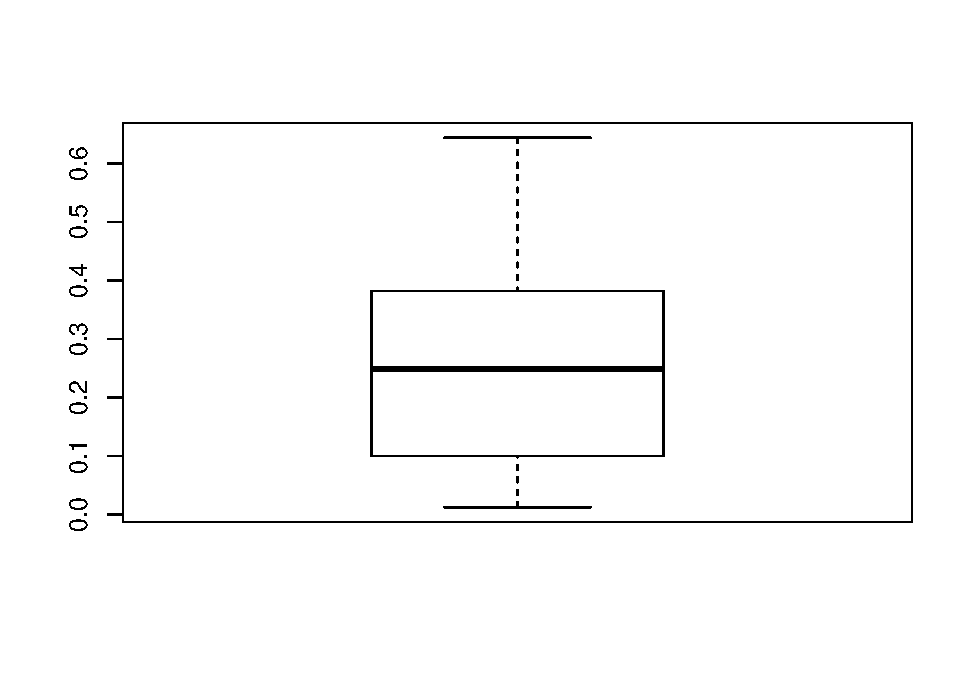
\includegraphics{Bagnard_Gaustad_Hartman_Leung_Lab_3_files/figure-latex/unnamed-chunk-97-1.pdf}

\textbf{Model 3 CLM Assumptions:}

\begin{itemize}
\item
  \textbf{MLR1 and 2}: Discussed earlier.
\item
  \textbf{MLR3} No perfect multicollinearity: We demonstrate that our
  independent variables are not perfectly multicolinear using the VIF
  function, and note that all of our variance inflation factors are less
  than 5.
\end{itemize}

\begin{Shaded}
\begin{Highlighting}[]
\KeywordTok{vif}\NormalTok{(model3)}
\end{Highlighting}
\end{Shaded}

\begin{verbatim}
##   logcrimJustEff         logpolpc logunweightedavg          density 
##         1.434962         1.370508         1.790625         2.104673 
##      logpctmin80 
##         1.069661
\end{verbatim}

\begin{itemize}
\tightlist
\item
  \textbf{MLR4'} Zero Conditional Mean: From the residual vs.~fitted
  chart below, we see that the mean of the residuals mostly lie along 0,
  except towards the left side of our chart where there are fewer data
  points. We can reasonably conclude that we satisfy MLR4.
\end{itemize}

\begin{Shaded}
\begin{Highlighting}[]
\KeywordTok{plot}\NormalTok{(model3, }\DataTypeTok{which =} \DecValTok{1}\NormalTok{)}
\end{Highlighting}
\end{Shaded}

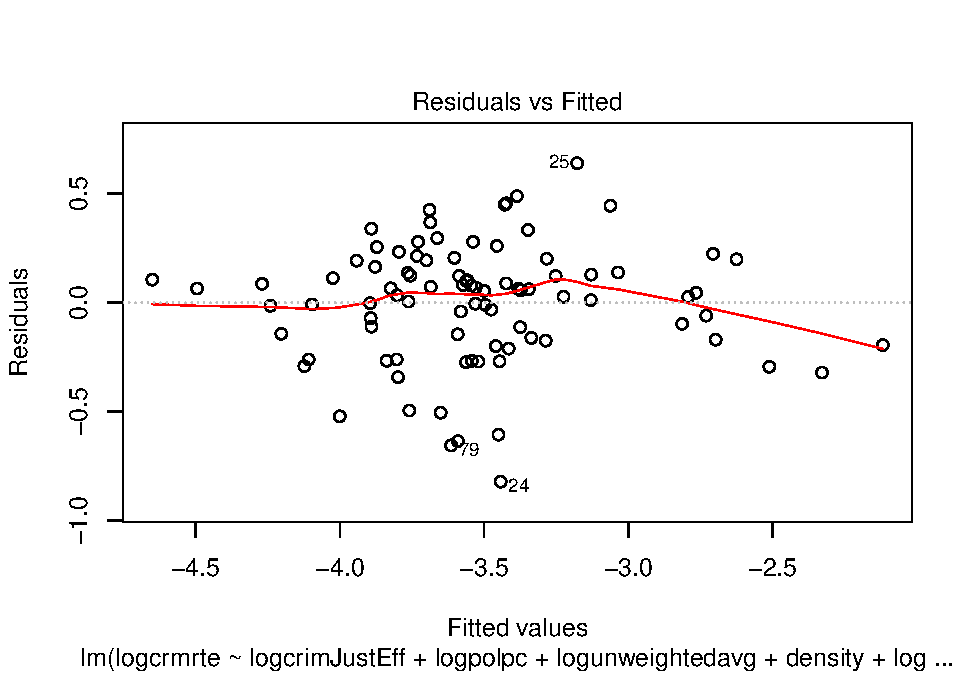
\includegraphics{Bagnard_Gaustad_Hartman_Leung_Lab_3_files/figure-latex/unnamed-chunk-99-1.pdf}

\begin{itemize}
\tightlist
\item
  \textbf{MLR5'} Spherical errors: We note from the residuals vs fitted
  chart above that we have some evidence of heteroscedasticity, since
  there are less datapoints on both the left and right of the chart. As
  a result, we use the vcovHC method to estimate a robust
  variance-covariance matrix using White and Huber's method and generate
  coefficients that are robust to heteroscedasticity.
\end{itemize}

\begin{Shaded}
\begin{Highlighting}[]
\KeywordTok{coeftest}\NormalTok{(model3, }\DataTypeTok{vcov=}\NormalTok{vcovHC)}
\end{Highlighting}
\end{Shaded}

\begin{verbatim}

t test of coefficients:

                  Estimate Std. Error t value  Pr(>|t|)    
(Intercept)      -7.621859   4.485588 -1.6992 0.0930291 .  
logcrimJustEff   -0.385566   0.094619 -4.0749 0.0001048 ***
logpolpc          0.339799   0.195159  1.7411 0.0853644 .  
logunweightedavg  0.998724   0.635210  1.5723 0.1196913    
density           0.072882   0.032747  2.2256 0.0287516 *  
logpctmin80       0.230646   0.038722  5.9564 5.988e-08 ***
---
Signif. codes:  0 '***' 0.001 '**' 0.01 '*' 0.05 '.' 0.1 ' ' 1
\end{verbatim}

\begin{itemize}
\tightlist
\item
  \textbf{MLR6'} Normality of errors: From the qqplot below, we see that
  the residuals in our model follow a fairly normal distribution. In
  addition, since we have a large sample size of 90 datapoints, we can
  rely on a version of the central limit theorem to assume normally
  distributed errors.
\end{itemize}

\begin{Shaded}
\begin{Highlighting}[]
\KeywordTok{plot}\NormalTok{(model3,}\DataTypeTok{which=}\DecValTok{2}\NormalTok{)}
\end{Highlighting}
\end{Shaded}

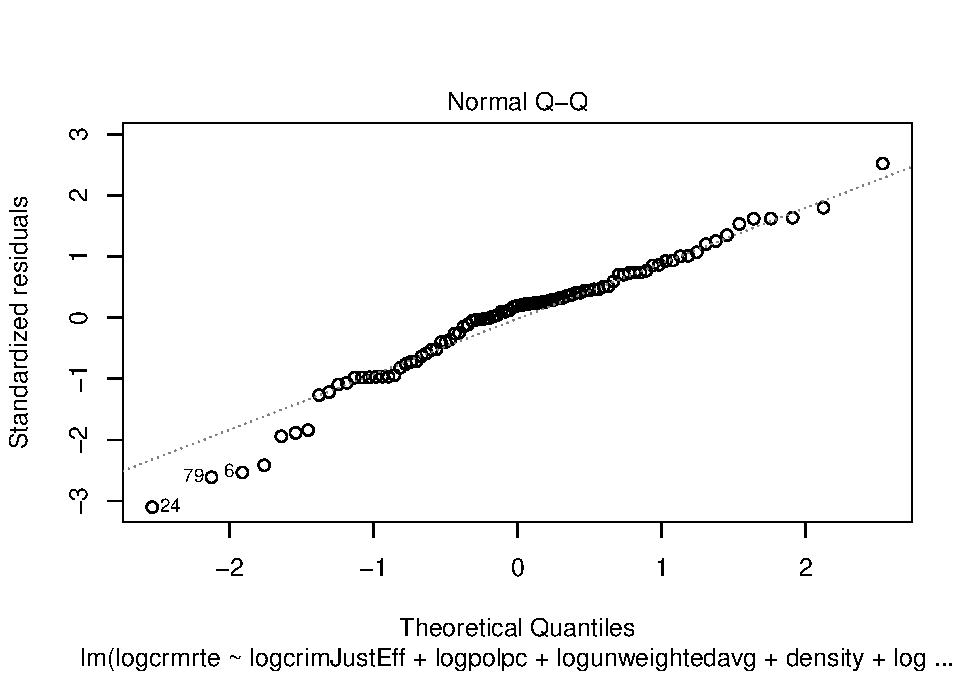
\includegraphics{Bagnard_Gaustad_Hartman_Leung_Lab_3_files/figure-latex/unnamed-chunk-101-1.pdf}

By satisfying these assumptions, we can expect that our coefficients are
approaching the true parameter values in probability.

\hypertarget{analysis}{%
\subsubsection{Analysis}\label{analysis}}

The model shows a good fit, with an adjusted R-squared of 0.72, meaning
that the model explains 72\% of the variation in crime.

After accounting for coefficients that are robust to heteroscedasticity,
we note only three them have statistical significance at the 95\% level
or better. These are criminal justice efficiency, minority percentages
and density.

\textbf{Interpretation of coefficients (Assuming ceterus paribus):}

Positive coefficients: * Police presence: If we increase police per
capita by 1 percent, we expect the crime rate to increase by 0.28\%. *
AllWages: If we increase wages by 1 percent, we expect the crime rate to
increase by 0.94\% * Density: If we increase density by 1 person per
square mile, we expect the crime rate to increase by 8\% * Percentage of
minorities: If the percentage of minorities increase by 1\%, we expect
the crime rate to increase by 0.24\%

Negative coefficients: * Criminal justice efficiency: If we increase the
criminal justice efficiency by 1\%, we expect the crime rate to decrease
by 0.42\%.

\hypertarget{results}{%
\subsubsection{Results:}\label{results}}

\hypertarget{comparison-of-regression-models}{%
\subsection{Comparison of Regression
Models}\label{comparison-of-regression-models}}

*\textbf{Can anyone figure out why logcrimJustEff is on 2 lines?}

\begin{Shaded}
\begin{Highlighting}[]
\KeywordTok{stargazer}\NormalTok{(mod1,model2,model3,}\DataTypeTok{type=}\StringTok{"text"}\NormalTok{)}
\end{Highlighting}
\end{Shaded}

\begin{verbatim}

========================================================================================
                                            Dependent variable:                         
                    --------------------------------------------------------------------
                          logcrmrte                          logcrmrte                  
                             (1)                    (2)                    (3)          
----------------------------------------------------------------------------------------
unweighted_avg_wage        0.006***                                                     
                           (0.001)                                                      
                                                                                        
logcrimJustEff            -0.434***                                                     
                           (0.076)                                                      
                                                                                        
logcrimJustEff                                   -0.260***              -0.386***       
                                                  (0.077)                (0.064)        
                                                                                        
logpolpc                                          0.333**                0.340***       
                                                  (0.146)                (0.108)        
                                                                                        
log(allWages)                                      0.501                                
                                                  (0.483)                               
                                                                                        
logtaxpc                                           0.036                                
                                                  (0.162)                               
                                                                                        
density)                                          0.405***                              
                                                  (0.116)                               
                                                                                        
logunweightedavg                                                         0.999***       
                                                                         (0.372)        
                                                                                        
density                                                                  0.073**        
                                                                         (0.029)        
                                                                                        
logpctmin80                                                              0.231***       
                                                                         (0.034)        
                                                                                        
Constant                  -6.300***                -6.479               -7.622***       
                           (0.374)                (4.092)                (2.394)        
                                                                                        
----------------------------------------------------------------------------------------
Observations                  89                     89                     89          
R2                          0.469                  0.586                  0.726         
Adjusted R2                 0.456                  0.561                  0.709         
Residual Std. Error    0.385 (df = 86)        0.346 (df = 83)        0.282 (df = 83)    
F Statistic         37.906*** (df = 2; 86) 23.532*** (df = 5; 83) 43.936*** (df = 5; 83)
========================================================================================
Note:                                                        *p<0.1; **p<0.05; ***p<0.01
\end{verbatim}

Comparing the 3 models, we see that our adjusted R2 value has steadily
increased from 0.456-0.732 as we introduce more covariates which
indicates that we were able to explain more variation in our model not
purely by increasing the number of indepedent variables.

At the same time, our standard errors have decreased \textbf{insert more
commentary on standard errors}.

We see that by expanding our definitions of criminal justice efficiency
and economic opportunity between model 1 and model 3 lowered the
coefficients for logcrimJustEff and allWages. This is most likely
because that we were able to better explain the effects with our newer
variables.

Comment on practical significance after week 12

\hypertarget{conclusion}{%
\section{Conclusion}\label{conclusion}}

\hypertarget{policy-recommendations}{%
\subsection{Policy Recommendations}\label{policy-recommendations}}

Given that across all 3 models, we show that both criminal justice
efficiency and tax revenues per capita have negative correlations to
crime rate, we propose the policy recommendations below to address these
issues. In addition, since minority percentages and density were found
to be highly significant in the model 3, we believe our recommendations
will be of particularly help to those running for political office in
counties with a high percentage of minorities or dense urban
populations.

\begin{enumerate}
\def\labelenumi{\arabic{enumi}.}
\item
  Since increasing both criminal justice and tax revenues are negatively
  correlated, we propose providing more funding for the local justice
  system.
\item
  While increasing taxes on constituents may be difficult politically
  and may cost candidates the ballot, candidates can instead try to
  attract investment to bring more jobs with higher wages so you can
  increase revenues.
\item
  Candidates can also propose to levy taxes on things that could lead to
  crimes or violence such as alcohol and weapons.
\item
  Given the significance and relatively large coefficient size of
  percentage minority, candidates should enroll local law enforcement
  into bias training.
\end{enumerate}

\hypertarget{ommitted-variables}{%
\subsection{Ommitted Variables}\label{ommitted-variables}}

\begin{longtable}[]{@{}l@{}}
\toprule
Expected correlation between omitted and included
variables\tabularnewline
\midrule
\endhead
\bottomrule
\end{longtable}

\begin{longtable}[]{@{}llll@{}}
\toprule
\begin{minipage}[b]{0.18\columnwidth}\raggedright
Omitted Variable\strut
\end{minipage} & \begin{minipage}[b]{0.19\columnwidth}\raggedright
Crime Rate (\(B_k\))\strut
\end{minipage} & \begin{minipage}[b]{0.31\columnwidth}\raggedright
Criminal Justice Effectiveness\strut
\end{minipage} & \begin{minipage}[b]{0.20\columnwidth}\raggedright
Economic Conditions\strut
\end{minipage}\tabularnewline
\midrule
\endhead
\begin{minipage}[t]{0.18\columnwidth}\raggedright
Education\strut
\end{minipage} & \begin{minipage}[t]{0.19\columnwidth}\raggedright
-\strut
\end{minipage} & \begin{minipage}[t]{0.31\columnwidth}\raggedright
unknown\strut
\end{minipage} & \begin{minipage}[t]{0.20\columnwidth}\raggedright
+\strut
\end{minipage}\tabularnewline
\begin{minipage}[t]{0.18\columnwidth}\raggedright
Social Services\strut
\end{minipage} & \begin{minipage}[t]{0.19\columnwidth}\raggedright
-\strut
\end{minipage} & \begin{minipage}[t]{0.31\columnwidth}\raggedright
unknown\strut
\end{minipage} & \begin{minipage}[t]{0.20\columnwidth}\raggedright
unknown\strut
\end{minipage}\tabularnewline
\begin{minipage}[t]{0.18\columnwidth}\raggedright
Unemployment\strut
\end{minipage} & \begin{minipage}[t]{0.19\columnwidth}\raggedright
+\strut
\end{minipage} & \begin{minipage}[t]{0.31\columnwidth}\raggedright
unknown\strut
\end{minipage} & \begin{minipage}[t]{0.20\columnwidth}\raggedright
-\strut
\end{minipage}\tabularnewline
\begin{minipage}[t]{0.18\columnwidth}\raggedright
Gang Activity\strut
\end{minipage} & \begin{minipage}[t]{0.19\columnwidth}\raggedright
+\strut
\end{minipage} & \begin{minipage}[t]{0.31\columnwidth}\raggedright
-\strut
\end{minipage} & \begin{minipage}[t]{0.20\columnwidth}\raggedright
-\strut
\end{minipage}\tabularnewline
\bottomrule
\end{longtable}

The 4 major identified ommited variables are shown above.

\begin{itemize}
\tightlist
\item
  Education is an important variable because of demographic insights it
  provides. First, adults with higher education are less likely to
  participate in Crime and are more likely to have better economic
  opportunity. Second, a strong school system is also likely correlated
  with less youth crime. Because of these expected correlations we are
  likely overestimating the economic conditions coefficient estimate.
\item
  Available Social Services could also lower crime. Citizens with strong
  social services support have more options to get help when they lack
  means for purchasing basic life needs. However this is more difficult
  to predict, as some social service projects, like homeless shelters,
  could lead to more criminal activity.
\item
  Unemployment is used as an important indicator of economic health and
  opportunity. This is would be highly correlated to economic conditions
  variables like sum of wages. This indicator variable if added to the
  model would decrease the magnitude of the sum of wage means
  coefficient estimate.\\
\item
  Gang or Organized Crime is special case of crime that contains unique
  causes. It is expected that it would be negatively correlated with
  criminal justice effectiveness as large social pressures prevent
  witnesses from supporting prosecution. Gang crime is also negatively
  correlated with economic conditions. From these assumed correlations,
  we can say that criminal justice effectiveness and economic conditions
  are both underestimated compared to including gang activity
  operationalized variable in the model.
\end{itemize}

\hypertarget{research-recommendations}{%
\subsection{Research Recommendations}\label{research-recommendations}}

We have shown in this report 3 different models that seek to explain and
model changes in the crime rate in North Carolina in 1980. We start with
the fundamental premise that crime is caused by both criminal justice
efficiency and economic conditions, and further develop our definition
of these two key explanatory variables which each new model.

In Model 3, we were able to explain up to 73\% of the variation in our
data, and found statistical significance at the 95\% level or better for
each of our covariates. Of these, we believe that increasing the
efficiency of the criminal justice system and tax revenues were the most
important, particularly for counties with high density and minority
populations. However, our findings should be noted with caution as we
were unable to study the effect of several ommitted variables including
education, availability of social services, unemployment rates and the
presence of organized crime. Had we been able to collect data on these
variables and apply them in our model, we believe we could increase
accuracy without bias.

\hypertarget{appendix}{%
\section{Appendix}\label{appendix}}

\begin{Shaded}
\begin{Highlighting}[]
\KeywordTok{options}\NormalTok{(}\DataTypeTok{repr.plot.width=}\DecValTok{8}\NormalTok{, }\DataTypeTok{repr.plot.height=}\DecValTok{4}\NormalTok{)}
\CommentTok{#myData<-myData[, c("crmrte", "prbarr", "prbconv", "prbpris", "avgsen", "polpc", "density", "taxpc",}
\CommentTok{#           "pctmin80", "wcon", "wtuc", "wtrd", "wfir", "wser", "wmfg", "wfed", "wsta", "wloc",}
\CommentTok{#           "mix", "pctymle")]}
\NormalTok{myData<-dfCrime }\OperatorTok\StringTok{ }\KeywordTok{filter}\NormalTok{(other}\OperatorTok{==}\DecValTok{1}\NormalTok{)}
\NormalTok{myData<-myData[, }\KeywordTok{c}\NormalTok{(}\StringTok{"logcrmrte"}\NormalTok{, }\StringTok{"logprbarr"}\NormalTok{, }\StringTok{"logprbconv"}\NormalTok{, }\StringTok{"logprbpris"}\NormalTok{, }\StringTok{"logavgsen"}\NormalTok{, }\StringTok{"logpolpc"}\NormalTok{, }\StringTok{"logtaxpc"}\NormalTok{,}
           \StringTok{"logpctmin80"}\NormalTok{, }\StringTok{"logwcon"}\NormalTok{, }\StringTok{"logwtuc"}\NormalTok{, }\StringTok{"logwtrd"}\NormalTok{, }\StringTok{"logwfir"}\NormalTok{, }\StringTok{"logwser"}\NormalTok{, }\StringTok{"logwmfg"}\NormalTok{, }\StringTok{"logwfed"}\NormalTok{, }\StringTok{"logwsta"}\NormalTok{, }\StringTok{"logwloc"}\NormalTok{,}
           \StringTok{"logmix"}\NormalTok{, }\StringTok{"logpctymle"}\NormalTok{)]}
\NormalTok{r0 <-}\StringTok{ }\NormalTok{myData }\OperatorTok\StringTok{ }\KeywordTok{correlate}\NormalTok{() }\OperatorTok\StringTok{ }\KeywordTok{network_plot}\NormalTok{(}\DataTypeTok{min_cor=}\NormalTok{.}\DecValTok{25}\NormalTok{)}
\end{Highlighting}
\end{Shaded}

\begin{verbatim}

Correlation method: 'pearson'
Missing treated using: 'pairwise.complete.obs'
\end{verbatim}

\begin{Shaded}
\begin{Highlighting}[]
\NormalTok{myData<-dfCrime }\OperatorTok\StringTok{ }\KeywordTok{filter}\NormalTok{(central}\OperatorTok{==}\DecValTok{1}\NormalTok{)}
\NormalTok{myData<-myData[, }\KeywordTok{c}\NormalTok{(}\StringTok{"logcrmrte"}\NormalTok{, }\StringTok{"logprbarr"}\NormalTok{, }\StringTok{"logprbconv"}\NormalTok{, }\StringTok{"logprbpris"}\NormalTok{, }\StringTok{"logavgsen"}\NormalTok{, }\StringTok{"logpolpc"}\NormalTok{, }\StringTok{"logtaxpc"}\NormalTok{,}
           \StringTok{"logpctmin80"}\NormalTok{, }\StringTok{"logwcon"}\NormalTok{, }\StringTok{"logwtuc"}\NormalTok{, }\StringTok{"logwtrd"}\NormalTok{, }\StringTok{"logwfir"}\NormalTok{, }\StringTok{"logwser"}\NormalTok{, }\StringTok{"logwmfg"}\NormalTok{, }\StringTok{"logwfed"}\NormalTok{, }\StringTok{"logwsta"}\NormalTok{, }\StringTok{"logwloc"}\NormalTok{,}
           \StringTok{"logmix"}\NormalTok{, }\StringTok{"logpctymle"}\NormalTok{)]}
\NormalTok{r1 <-}\StringTok{ }\NormalTok{myData }\OperatorTok\StringTok{ }\KeywordTok{correlate}\NormalTok{() }\OperatorTok\StringTok{ }\KeywordTok{network_plot}\NormalTok{(}\DataTypeTok{min_cor=}\NormalTok{.}\DecValTok{25}\NormalTok{)}
\end{Highlighting}
\end{Shaded}

\begin{verbatim}

Correlation method: 'pearson'
Missing treated using: 'pairwise.complete.obs'
\end{verbatim}

\begin{Shaded}
\begin{Highlighting}[]
\NormalTok{myData<-dfCrime }\OperatorTok\StringTok{ }\KeywordTok{filter}\NormalTok{(west}\OperatorTok{==}\DecValTok{1}\NormalTok{)}
\NormalTok{myData<-myData[, }\KeywordTok{c}\NormalTok{(}\StringTok{"logcrmrte"}\NormalTok{, }\StringTok{"logprbarr"}\NormalTok{, }\StringTok{"logprbconv"}\NormalTok{, }\StringTok{"logprbpris"}\NormalTok{, }\StringTok{"logavgsen"}\NormalTok{, }\StringTok{"logpolpc"}\NormalTok{, }\StringTok{"logtaxpc"}\NormalTok{,}
           \StringTok{"logpctmin80"}\NormalTok{, }\StringTok{"logwcon"}\NormalTok{, }\StringTok{"logwtuc"}\NormalTok{, }\StringTok{"logwtrd"}\NormalTok{, }\StringTok{"logwfir"}\NormalTok{, }\StringTok{"logwser"}\NormalTok{, }\StringTok{"logwmfg"}\NormalTok{, }\StringTok{"logwfed"}\NormalTok{, }\StringTok{"logwsta"}\NormalTok{, }\StringTok{"logwloc"}\NormalTok{,}
           \StringTok{"logmix"}\NormalTok{, }\StringTok{"logpctymle"}\NormalTok{)]}
\NormalTok{r2 <-}\StringTok{ }\NormalTok{myData }\OperatorTok\StringTok{ }\KeywordTok{correlate}\NormalTok{() }\OperatorTok\StringTok{ }\KeywordTok{network_plot}\NormalTok{(}\DataTypeTok{min_cor=}\NormalTok{.}\DecValTok{25}\NormalTok{)}
\end{Highlighting}
\end{Shaded}

\begin{verbatim}

Correlation method: 'pearson'
Missing treated using: 'pairwise.complete.obs'
\end{verbatim}

\begin{Shaded}
\begin{Highlighting}[]
\KeywordTok{grid.arrange}\NormalTok{(}\KeywordTok{arrangeGrob}\NormalTok{(r1, }\DataTypeTok{bottom =} \StringTok{'Central Region Correlation Plot'}\NormalTok{), }\DataTypeTok{ncol=}\DecValTok{1}\NormalTok{)}
\end{Highlighting}
\end{Shaded}

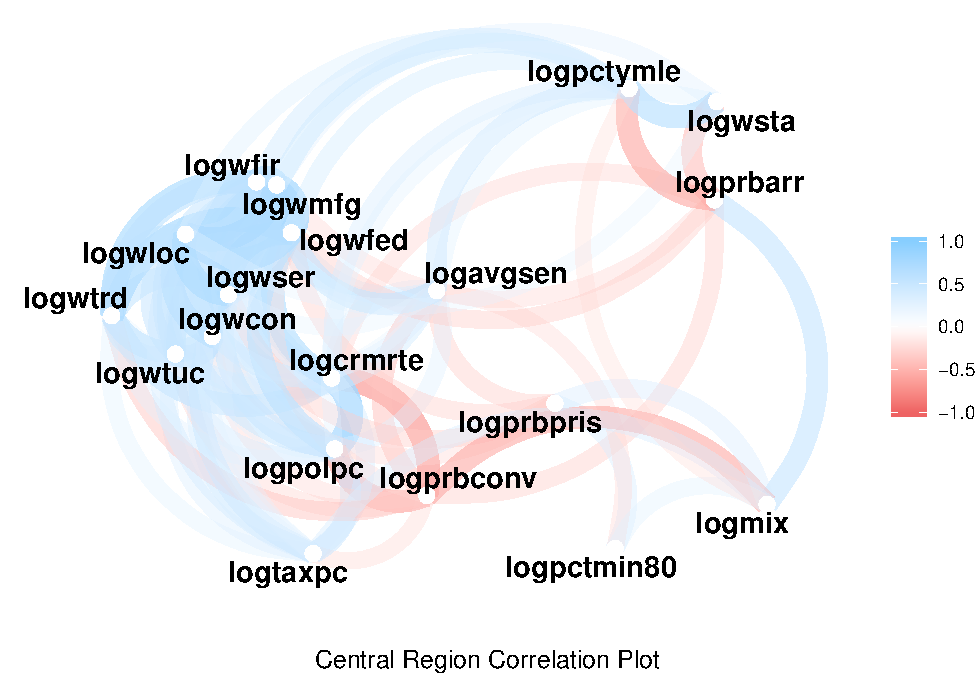
\includegraphics{Bagnard_Gaustad_Hartman_Leung_Lab_3_files/figure-latex/unnamed-chunk-103-1.pdf}

\begin{Shaded}
\begin{Highlighting}[]
\KeywordTok{grid.arrange}\NormalTok{(}\KeywordTok{arrangeGrob}\NormalTok{(r2, }\DataTypeTok{bottom =} \StringTok{'Western Region Correlation Plot'}\NormalTok{), }\DataTypeTok{ncol=}\DecValTok{1}\NormalTok{)}
\end{Highlighting}
\end{Shaded}

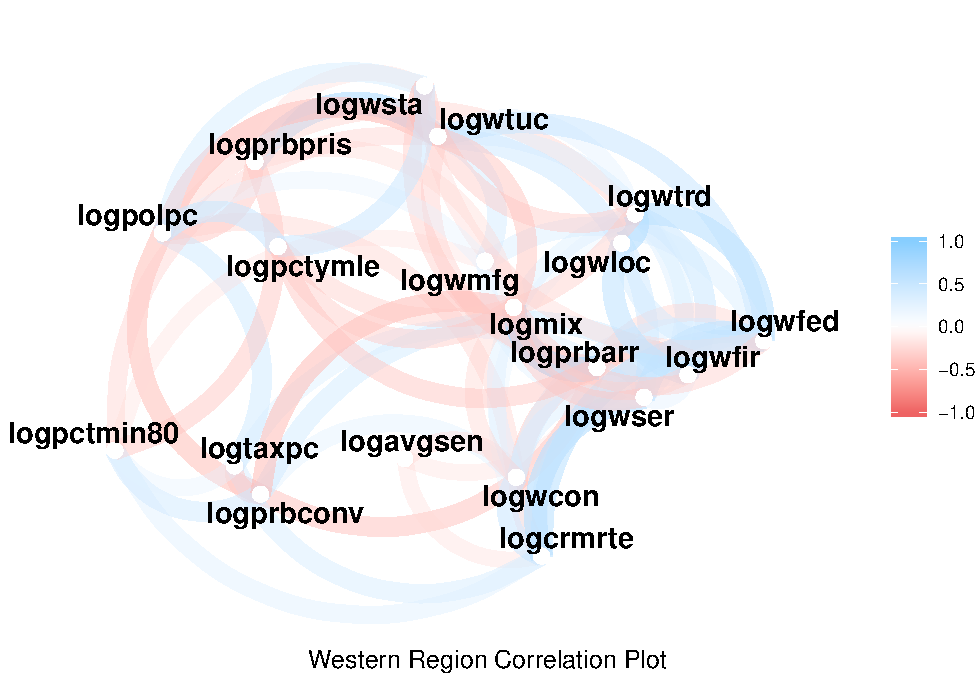
\includegraphics{Bagnard_Gaustad_Hartman_Leung_Lab_3_files/figure-latex/unnamed-chunk-103-2.pdf}

\begin{Shaded}
\begin{Highlighting}[]
\KeywordTok{grid.arrange}\NormalTok{(}\KeywordTok{arrangeGrob}\NormalTok{(r0, }\DataTypeTok{bottom =} \StringTok{'Other Region Correlation Plot'}\NormalTok{), }\DataTypeTok{ncol=}\DecValTok{1}\NormalTok{)}
\end{Highlighting}
\end{Shaded}

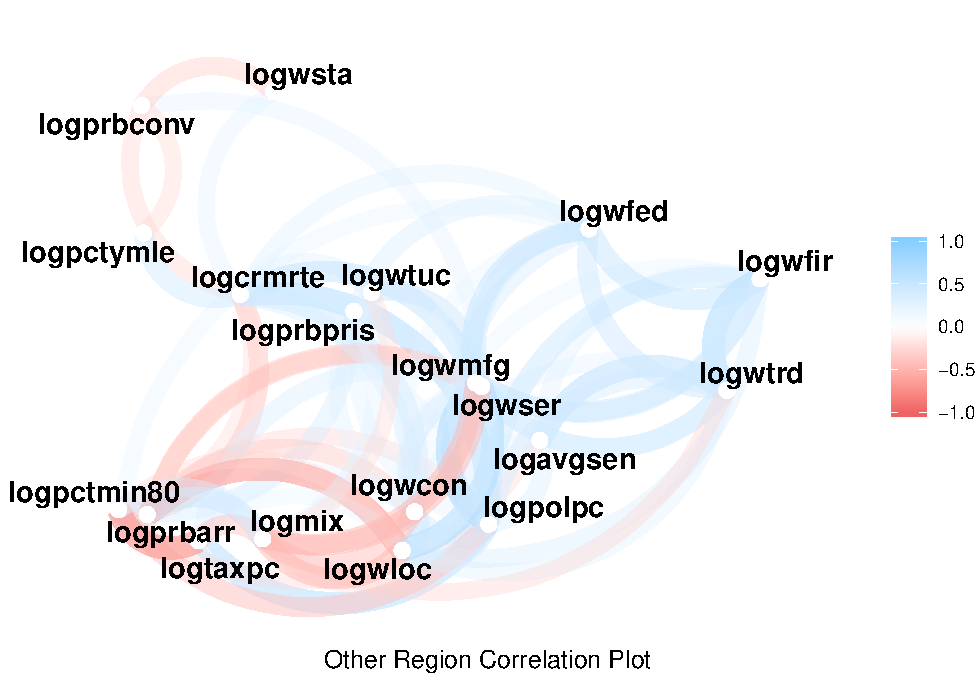
\includegraphics{Bagnard_Gaustad_Hartman_Leung_Lab_3_files/figure-latex/unnamed-chunk-103-3.pdf}

\begin{Shaded}
\begin{Highlighting}[]
\NormalTok{myData<-dfCrime }\OperatorTok\StringTok{ }\KeywordTok{filter}\NormalTok{(urban}\OperatorTok{==}\DecValTok{0}\NormalTok{)}
\NormalTok{myData<-myData[, }\KeywordTok{c}\NormalTok{(}\StringTok{"logcrmrte"}\NormalTok{, }\StringTok{"logprbarr"}\NormalTok{, }\StringTok{"logprbconv"}\NormalTok{, }\StringTok{"logprbpris"}\NormalTok{, }\StringTok{"logavgsen"}\NormalTok{, }\StringTok{"logpolpc"}\NormalTok{, }\StringTok{"logtaxpc"}\NormalTok{,}
           \StringTok{"logpctmin80"}\NormalTok{, }\StringTok{"logwcon"}\NormalTok{, }\StringTok{"logwtuc"}\NormalTok{, }\StringTok{"logwtrd"}\NormalTok{, }\StringTok{"logwfir"}\NormalTok{, }\StringTok{"logwser"}\NormalTok{, }\StringTok{"logwmfg"}\NormalTok{, }\StringTok{"logwfed"}\NormalTok{, }\StringTok{"logwsta"}\NormalTok{, }\StringTok{"logwloc"}\NormalTok{,}
           \StringTok{"logmix"}\NormalTok{, }\StringTok{"logpctymle"}\NormalTok{)]}
\NormalTok{r0 <-}\StringTok{ }\NormalTok{myData }\OperatorTok\StringTok{ }\KeywordTok{correlate}\NormalTok{() }\OperatorTok\StringTok{ }\KeywordTok{network_plot}\NormalTok{(}\DataTypeTok{min_cor=}\NormalTok{.}\DecValTok{25}\NormalTok{)}
\end{Highlighting}
\end{Shaded}

\begin{verbatim}

Correlation method: 'pearson'
Missing treated using: 'pairwise.complete.obs'
\end{verbatim}

\begin{Shaded}
\begin{Highlighting}[]
\NormalTok{myData<-dfCrime }\OperatorTok\StringTok{ }\KeywordTok{filter}\NormalTok{(urban}\OperatorTok{==}\DecValTok{1}\NormalTok{)}
\NormalTok{myData<-myData[, }\KeywordTok{c}\NormalTok{(}\StringTok{"logcrmrte"}\NormalTok{, }\StringTok{"logprbarr"}\NormalTok{, }\StringTok{"logprbconv"}\NormalTok{, }\StringTok{"logprbpris"}\NormalTok{, }\StringTok{"logavgsen"}\NormalTok{, }\StringTok{"logpolpc"}\NormalTok{,  }\StringTok{"logtaxpc"}\NormalTok{,}
           \StringTok{"logpctmin80"}\NormalTok{, }\StringTok{"logwcon"}\NormalTok{, }\StringTok{"logwtuc"}\NormalTok{, }\StringTok{"logwtrd"}\NormalTok{, }\StringTok{"logwfir"}\NormalTok{, }\StringTok{"logwser"}\NormalTok{, }\StringTok{"logwmfg"}\NormalTok{, }\StringTok{"logwfed"}\NormalTok{, }\StringTok{"logwsta"}\NormalTok{, }\StringTok{"logwloc"}\NormalTok{,}
           \StringTok{"logmix"}\NormalTok{, }\StringTok{"logpctymle"}\NormalTok{)]}
\NormalTok{r1 <-}\StringTok{ }\NormalTok{myData }\OperatorTok\StringTok{ }\KeywordTok{correlate}\NormalTok{() }\OperatorTok\StringTok{ }\KeywordTok{network_plot}\NormalTok{(}\DataTypeTok{min_cor=}\NormalTok{.}\DecValTok{25}\NormalTok{)}
\end{Highlighting}
\end{Shaded}

\begin{verbatim}

Correlation method: 'pearson'
Missing treated using: 'pairwise.complete.obs'
\end{verbatim}

\begin{Shaded}
\begin{Highlighting}[]
\KeywordTok{grid.arrange}\NormalTok{(}\KeywordTok{arrangeGrob}\NormalTok{(r0, }\DataTypeTok{bottom =} \StringTok{'Non-Urban Correlation Plot'}\NormalTok{), }\DataTypeTok{ncol=}\DecValTok{1}\NormalTok{)}
\end{Highlighting}
\end{Shaded}

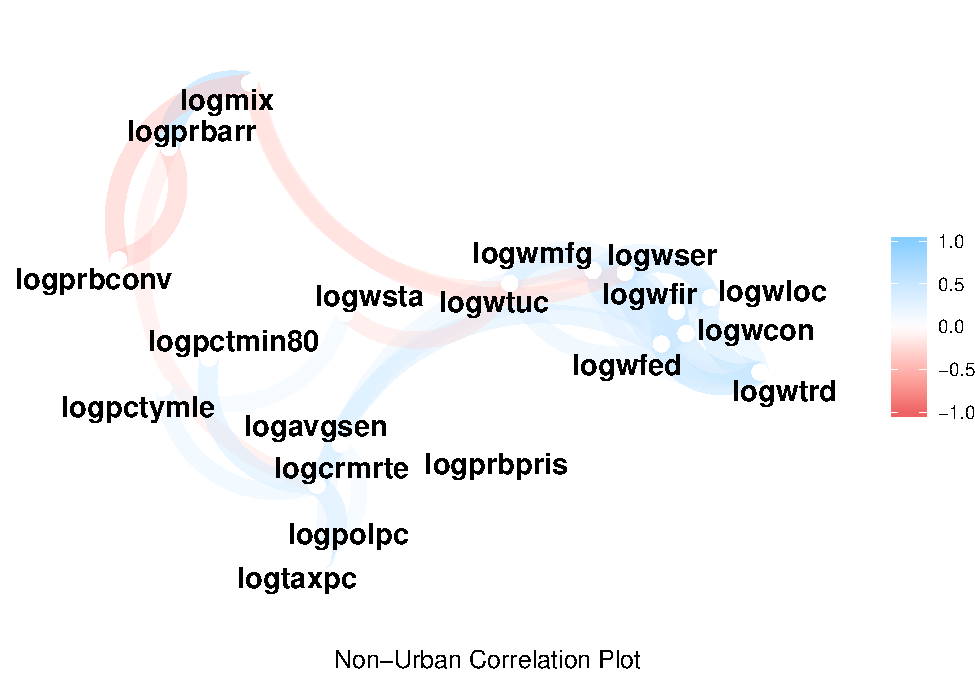
\includegraphics{Bagnard_Gaustad_Hartman_Leung_Lab_3_files/figure-latex/unnamed-chunk-103-4.pdf}

\begin{Shaded}
\begin{Highlighting}[]
\KeywordTok{grid.arrange}\NormalTok{(}\KeywordTok{arrangeGrob}\NormalTok{(r1, }\DataTypeTok{bottom =} \StringTok{'Urban Correlation Plot'}\NormalTok{), }\DataTypeTok{ncol=}\DecValTok{1}\NormalTok{)}
\end{Highlighting}
\end{Shaded}

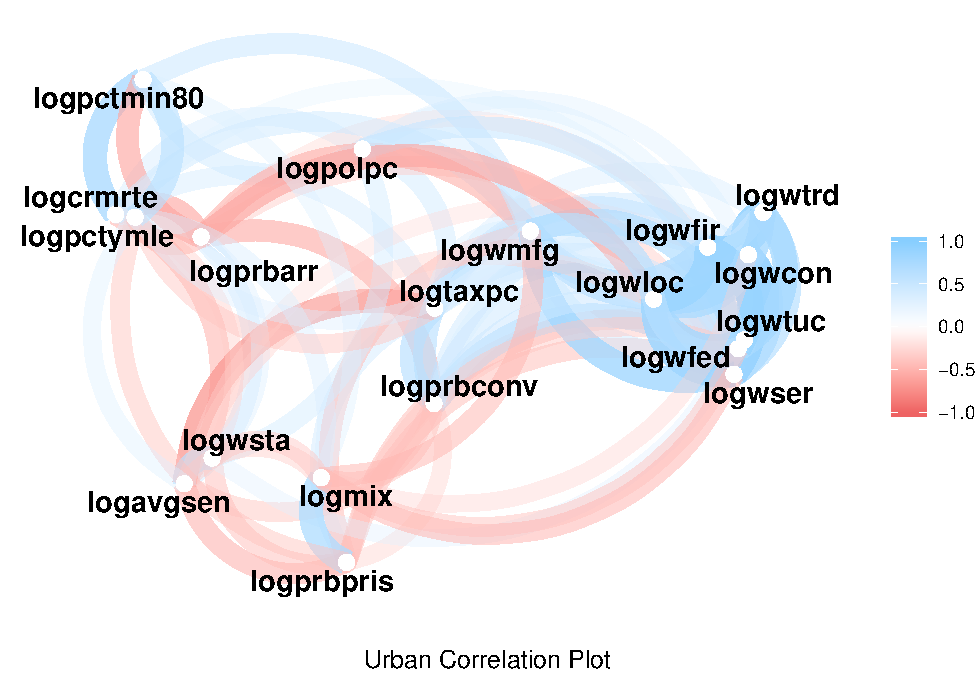
\includegraphics{Bagnard_Gaustad_Hartman_Leung_Lab_3_files/figure-latex/unnamed-chunk-103-5.pdf}


\end{document}
